%%%%%%%%%%%%%%%%%%%%%%%%%%%%%%%%%%%%%%%%%
% Masters/Doctoral Thesis 
% LaTeX Template
% Version 2.5 (27/8/17)
%
% This template was downloaded from:
% http://www.LaTeXTemplates.com
%
% Version 2.x major modifications by:
% Vel (vel@latextemplates.com)
%
% This template is based on a template by:
% Steve Gunn (http://users.ecs.soton.ac.uk/srg/softwaretools/document/templates/)
% Sunil Patel (http://www.sunilpatel.co.uk/thesis-template/)
%
% Template license:
% CC BY-NC-SA 3.0 (http://creativecommons.org/licenses/by-nc-sa/3.0/)
%
%%%%%%%%%%%%%%%%%%%%%%%%%%%%%%%%%%%%%%%%%

%----------------------------------------------------------------------------------------
%	PACKAGES AND OTHER DOCUMENT CONFIGURATIONS
%----------------------------------------------------------------------------------------

\documentclass[
11pt, % The default document font size, options: 10pt, 11pt, 12pt
%oneside, % Two side (alternating margins) for binding by default, uncomment to switch to one side
ngerman, % ngerman for German
singlespacing, % Single line spacing, alternatives: onehalfspacing or doublespacing
%draft, % Uncomment to enable draft mode (no pictures, no links, overfull hboxes indicated)
%nolistspacing, % If the document is onehalfspacing or doublespacing, uncomment this to set spacing in lists to single
%liststotoc, % Uncomment to add the list of figures/tables/etc to the table of contents
%toctotoc, % Uncomment to add the main table of contents to the table of contents
%parskip, % Uncomment to add space between paragraphs
%nohyperref, % Uncomment to not load the hyperref package
headsepline, % Uncomment to get a line under the header
%chapterinoneline, % Uncomment to place the chapter title next to the number on one line
%consistentlayout, % Uncomment to change the layout of the declaration, abstract and acknowledgements pages to match the default layout
]{MastersDoctoralThesis} % The class file specifying the document structure

\usepackage[utf8]{inputenc} % Required for inputting international characters
\usepackage[T1]{fontenc} % Output font encoding for international characters

\usepackage{mathpazo} % Use the Palatino font by default

\usepackage{svg}

\usepackage[chapter]{minted} % Style sourcecode easily

\renewcommand\listingscaption{Sourcecode} % Show chapter number in listing caption

\usepackage[backend=bibtex,style=authoryear,natbib=true, maxbibnames=99, dashed=false]{biblatex} % Use the bibtex backend with the authoryear citation style (which resembles APA)

\addbibresource{literatur.bib} % The filename of the bibliography

\usepackage[autostyle=true]{csquotes} % Required to generate language-dependent quotes in the bibliography

% package for colored text
% black,white,green,red,blue,yellow,cyan,magenta
\usepackage{color}

% package for colored tables
\usepackage{colortbl}

% todos im Text
\usepackage{todonotes}

% Glossar und Abkürzungen
\usepackage[acronym]{glossaries}

% Buchstaben statt Zahlen in Aufzählungen
\usepackage{enumitem}

% Diagramme
\usepackage{pgfplots}

% Codehighlighting
%\usepackage{listings}

% package to break URL
\usepackage{url}
\def\UrlBreaks{\do\/\do-}
\usepackage{breakurl}

% Define some commands to keep the formatting separated from the content 
\newcommand{\term}[1]{\textit{#1}}


%----------------------------------------------------------------------------------------
%	MARGIN SETTINGS
%----------------------------------------------------------------------------------------

\geometry{
	paper=a4paper, % Change to letterpaper for US letter
	inner=2.5cm, % Inner margin
	outer=3.8cm, % Outer margin
	bindingoffset=.5cm, % Binding offset
	top=1.5cm, % Top margin
	bottom=1.5cm, % Bottom margin
	%showframe, % Uncomment to show how the type block is set on the page
}

%----------------------------------------------------------------------------------------
%	THESIS INFORMATION
%----------------------------------------------------------------------------------------

\thesistitle{Pay2Mail - Entwicklung eines Systems zur transparenten Darstellung und absendergesteuerten Priorisierung von E-Mail Warteschlangen} % Your thesis title, this is used in the title and abstract, print it elsewhere with \ttitle

\author{Alexander \textsc{Strutz}} % Your name, this is used in the title page and abstract, print it elsewhere with \authorname

\degree{Master of Science} % Your degree name, this is used in the title page and abstract, print it elsewhere with \degreename

\subject{Web Science} % Your subject area, this is not currently used anywhere in the template, print it elsewhere with \subjectname

\keywords{} % Keywords for your thesis, this is not currently used anywhere in the template, print it elsewhere with \keywordnames

\loadglsentries{Appendices/glossary}
\loadglsentries{Appendices/acronyms}
\makeglossaries

\AtBeginDocument{
\hypersetup{pdftitle=\ttitle} % Set the PDF's title to your title
\hypersetup{pdfauthor=\authorname} % Set the PDF's author to your name
\hypersetup{pdfkeywords=\keywordnames} % Set the PDF's keywords to your keywords
}

\begin{document}

\hypersetup{urlcolor=blue}

\frontmatter % Use roman page numbering style (i, ii, iii, iv...) for the pre-content pages

\pagestyle{plain} % Default to the plain heading style until the thesis style is called for the body content

%----------------------------------------------------------------------------------------
%	TITLE PAGE
%----------------------------------------------------------------------------------------

%!TEX root = ../main.tex

\begin{titlepage}

\begin{center}

% Logo Cologne University of Applied Sciences
\begin{figure}[!ht]
	\flushleft
		
\includegraphics[width=0.26\textwidth]{Figures/THlogoheader.pdf}
\end{figure}

\vspace{0.8cm}

% Title
\begin{rmfamily}
\vspace{0.5cm}
\begin{huge}
\textbf{\ttitle}\\	
\end{huge}
\vspace{0.5cm}
% \begin{LARGE}
% if needed with a \\subtitle\\
% \end{LARGE}
\end{rmfamily}

\vspace{1.6cm}


% Master Thesis 
\begin{LARGE}
\begin{scshape}
Masterthesis\\[0.8em]
\end{scshape}
\end{LARGE}

% elaborated by...
\begin{large}
von\\ 
\vspace{0.2cm}
\begin{LARGE}
Alexander Strutz\\
\end{LARGE}
\end{large}

\vspace{1.0cm}

% to obtain the M.Sc.
\begin{large}
zur Erlangung des Grades\\
\vspace{0.4cm}
\textsc{Master of Science (M.Sc.)}\\ 
\end{large}

\vspace{0.6cm}

% submitted at...
\begin{large}
an der\\ 
\vspace{0.2cm}
\begin{scshape}
TH Köln\\
Fakultät für Informatik und Ingenieurwissenschaften\\
\end{scshape}
\end{large}

\vspace{0.8cm}

% Course of Studies
\begin{large}
Studienfach\\ 
\vspace{0.2cm}
\textsc{Medieninformatik - Weaving the Web}
\end{large}


\vspace{1.0cm}

% author and supervisors
\begin{tabular}{rl}
        Erstprüfer:  &  Prof. Christian \textsc{Noss}\\
       					&  \small TH Köln, Advanced Media Institute \\[1.0em]
       Zweitprüfer:  &  Prof Dr. Mario \textsc{Winter} \\
       					&  \small TH Köln, Institut für Informatik\\[1.0em]
\end{tabular}

\vspace{0.6cm}

% location, months of submission
\begin{large}
Gummersbach, November 2022
\end{large}

\end{center}

\newpage
\thispagestyle{empty}

% contact details of author and supervisors
\begin{center}
\begin{tabular}{rl}
							&  \\[36.0em]
							
\large \textbf{Kontaktinformationen:}	&  	\quad \authorname \\
							&  	\quad Richardstraße 23\\
							&	\quad 40231 Düsseldorf\\
							&  	\quad astrutz@th-koeln.de\\[2.0em]
							
							&  	\quad Prof. Christian \textsc{Noss}\\
							&  	\quad TH Köln\\
							&  	\quad Advanced Media Institute\\
							&	\quad Steinmüllerallee 1\\
							&	\quad 51643 Gummersbach\\
							&  	\quad christian.noss@th-koeln.de\\[2.0em]
							
							&  	\quad Prof. Dr. Mario \textsc{Winter}\\
							&  	\quad TH Köln\\
							&  	\quad Institut für Informatik\\
							&	\quad Steinmüllerallee 1\\
							&	\quad 51643 Gummersbach\\
							&  	\quad mario.winter@th-koeln.de\\[2.0em]
\end{tabular}
\end{center}

\end{titlepage}


%----------------------------------------------------------------------------------------
%	ABSTRACT PAGE
%----------------------------------------------------------------------------------------

%!TEX root = ../main.tex

\chapter*{Abstract}
\addchaptertocentry{Abstract}
Write your abstract here. It should be structured like \enquote{introduction - solution - aim of the thesis}.


%----------------------------------------------------------------------------------------
%	LIST OF CONTENTS/FIGURES/TABLES PAGES
%----------------------------------------------------------------------------------------
{\hypersetup{linkcolor=black}
    \tableofcontents % Prints the main table of contents
    \setcounter{tocdepth}{2} % Workaround to empty list of figures/tables
    
    
    \listoffigures % Prints the list of figures
    \addcontentsline{toc}{chapter}{Abbildungsverzeichnis} % Adds line into table of contents
    
    \listoftables % Prints the list of tables
    \addcontentsline{toc}{chapter}{Tabellenverzeichnis} % Adds line into table of contents
    
    \renewcommand\listoflistingscaption{Sourcecodeverzeichnis}
    \listoflistings
    \addcontentsline{toc}{chapter}{Sourcecodeverzeichnis} % Adds line into table of contents
}

%----------------------------------------------------------------------------------------
%	ACRONYMS + GLOSSARY
%----------------------------------------------------------------------------------------

\setglossarystyle{list}
\printglossary[type=\acronymtype, title=Abkürzungsverzeichnis, toctitle=Abkürzungsverzeichnis, nonumberlist]
\addcontentsline{toc}{chapter}{Abkürzungsverzeichnis} % Adds line into table of contents

\glsaddallunused[\acronymtype]


\setglossarystyle{altlist}
\printglossary[nonumberlist]
\addcontentsline{toc}{chapter}{Glossar} % Adds line into table of contents

\glsaddallunused

%----------------------------------------------------------------------------------------
%	THESIS CONTENT - CHAPTERS
%----------------------------------------------------------------------------------------

\mainmatter % Begin numeric (1,2,3...) page numbering

\pagestyle{thesis} % Return the page headers back to the "thesis" style

% Include the chapters of the thesis as separate files from the Chapters folder
% Uncomment the lines as you write the chapters

%!TEX root = ../main.tex
% Chapter 1

\chapter{Einleitung}
\label{Einleitung}

Dieses Kapitel leitet in die grundlegende Thematik von E-Mails ein. Nach einer Erläuterung dieser Domäne wird das sich daraus ergebende Problemfeld beschrieben und mögliche Folgen dessen skizziert. Die Bearbeitung des Problemfelds ergibt eine Forschungsfrage, die diese Arbeit inhaltlich lenkt. Darüber hinaus wird die Vorgehensweise beschrieben, mit welcher die Forschungsfrage beantwortet werden soll.

\section{Kontext und Domäne}
\label{Kontext_und_Domaene}
Die E-Mail ist in den letzten drei Jahrzehnten zu einem der wichtigsten Kommunikationsmittel aufgestiegen. Diese Entwicklung lässt sich anhand verschiedener Faktoren beobachten.

Grundsätzlich ist die Anzahl der E-Mail Nutzer kontinuierlich gestiegen. Während 2002 nur 38\% der Bevölkerung in Deutschland das Internet für E-Mails nutzten, betrug der Wert im Jahr 2020 87\% \citep{SAEU2022}. Insbesondere in der Altersgruppe von 16 bis 64 Jahren gaben in einer Studie im Jahr 2020 über 90\% der Befragten an in den letzten drei Monaten E-Mails versendet oder empfangen zu haben \citep{StatistischesBundesamt2021}. Diese hohen Nutzerzahlen verdeutlichen die hohe Relevanz, die die E-Mail im alltäglichen Leben hat.

Ein weiterer Indikator ist die Anzahl der versendeten E-Mails, welche von 2000 (32,3 Milliarden) bis 2018 (848,1 Milliarden) um das 26-fache anstieg, Spam-Mails exkludiert \citep{MMG2018}. Auffällig ist insbesondere der Anstieg im Jahr 2017 um 146 Milliarden E-Mails. Dies ist zum Einen durch eine erhöhte Nutzung von natürlichen Personen, aber auch durch eine erhöhte Anzahl an \textit{technischen E-Mails} zu erklären.  \gls{technischeemail}s sind E-Mails, welche von Systemen automatisch versendet werden, zum Beispiel zur Registrierung von Nutzern, Information von Nutzern, Newslettern oder \acrfull{2fa}. Letztere erklärt den Anstieg des E-Mail Verkehrs von 2017, da in diesem Jahr die EU-Verordnung zur verpflichtenden Nutzung von 2FA in beispielsweise Online-Banking eingeführt wurde \citep{EuropaeischeKommission2017}. Dies hat zur Folge, dass bei jedem Login eine SMS, App-Benachrichtigung, E-Mail etc. versendet wird.

E-Mails lassen sich nicht nur anhand ihres Absenders (Mensch/System), sondern auch anhand ihres Zweckes unterscheiden. So sind die Einsatzzwecke vielfältig und umfassend. In einer Studie der \cite{MMG2020} gaben 63\% der Befragten an mit Firmen, 54\% mit Bekannten und Familie, 53\% mit Ämtern, 38\% mit Freunden und 20\% mit Lebenspartnern über E-Mails zu kommunizieren.

Die Nutzung in verschiedenen Kontexten hat zur Folge, dass E-Mails, insofern sie je nach Einsatzzweck nicht strikt in verschiedenen Konten sortiert sind, eine Sichtung benötigen. Eine solche Sichtung, auch \textit{\gls{triage}} genannt, bezeichnet den \emph{\glqq[...] Prozess, bei dem unbearbeitete E-Mails durchgesehen und entschieden wird, was damit zu tun ist.\grqq{}} \citep[S. 325]{Sarrafzadeh2019}. \gls{triage} ist, insbesondere im beruflichen Kontext, relevant für die persönliche Aufgabenverwaltung und die Produktivität. Die aus einer Triage entstehenden Handlungsschritte können die Beantwortung, das Lesen, das Löschen, das Sortieren oder die Archivierung einer E-Mail sein. \cite{Sarrafzadeh2019} identifizieren innerhalb der Triage drei Schritte: Priorisierung, Zurückstellung und Strategien zur Erleichterung der Wiedervorlage. Der Ablauf einer Triage ist als Flussdiagramm in Abbildung \ref{fig:triage_ablauf} dargestellt.

In der Priorisierung versucht der Nutzer die Intention von E-Mails und einen möglichen Handlungsbedarf zu identifizieren. Verschiedene Strategien zur Priorisierung werden im nächsten Absatz näher erläutert. Nachdem E-Mails ohne direkten Handlungsbedarf aussortiert wurden, wird in der Zurückstellung entschieden, welche E-Mails direkt und welche E-Mails vorerst nicht bearbeitet werden. Die Entscheidung über eine Zurückstellung wird insbesondere dadurch entschieden, ob Empfänger zeitnah eine Rückmeldung geben können und ob die E-Mail eine Dringlichkeit aufweist \citep[S. 327]{Sarrafzadeh2019}. Zurückgestellte E-Mails werden zu einem späteren Zeitpunkt beantwortet. Damit Empfänger diese Wiedervorlage als Aufgabe nicht vernachlässigen, werden Strategien zur Erleichterung angewendet. Diese Strategien sind individuell und können beispielsweise die Sortierung von E-Mails in verschiedenen Ordnern, das Markieren mit bestimmten Stichwörtern oder die Erinnerung über ToDo-Listen, Kalender und andere Tools sein.

\begin{figure}[!ht]
	\centering
		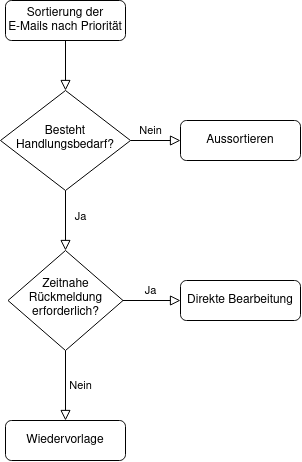
\includegraphics[width=0.5\textwidth]{Figures/Triage.png}
	\caption[Ablauf einer Triage]{Ablauf einer Triage nach \cite{Sarrafzadeh2019}}
	\label{fig:triage_ablauf}
\end{figure}

\noindent Da sowohl die Zurückstellung, als auch die Strategien zur Erleichterung der Wiedervorlage als Folgeaufgabe aus der Priorisierung entstehen, kann dieser eine übergeordnete Rolle zugewiesen werden. Hierbei entscheidend sind die Faktoren, die die Relevanz einer E-Mail für den Nutzer bestimmen. \cite{Dabbish2005} beobachteten, dass sowohl Absendercharakteristiken als auch der Nachrichteninhalt die Bewertung beeinflussen. So werden Nachrichten um bis zu 25\% wichtiger bewertet, wenn sie von Vorgesetzten, externen Kunden oder sonstigen Personen versendet werden, als wenn sie von Bekannten, engeren Arbeitskollegen oder allgemeinen Informationssystemen stammen \citep[S. 698]{Dabbish2005}. Beim Inhalt der Nachricht haben insbesondere Handlungsaufforderungen, sowie Forderungen nach Informationen einen Einfluss von bis zu 20\% \citep[S. 696]{Dabbish2005}. Dieser Einfluss kann durch eine zeitliche Frist vergrößert werden. Im professionellen Kontext implizieren sozial orientierte Inhalte ebenso wie eine Aufnahme des Empfängers in \acrshort{cc} eine geringere Priorität. Hervorzuheben ist, dass das Feld \textit{Priorität} einer E-Mail keinen Einfluss auf die Beurteilung nimmt \citep[S. 279 f.]{Whittaker1996}.

Ferner ist festzuhalten, dass sich die Vorgehensweise der Triage regional unterscheiden kann. So stellten \cite{Tang2009} unter anderem fest, dass Nutzer in Europa ihre E-Mails eher in verschiedenen Ordnern sortieren, während dies in asiatischen Ländern weniger der Fall ist. Eine Aussage zur Effizienz dieser Methoden kann nicht getroffen werden.

%----------------------------------------------------------------------------------------

\section{Problemfeld und Folgen}
\label{Problemfeld_und_Folgen}

Die angestiegene Relevanz der E-Mail im alltäglichen Leben bringt verschiedene Probleme mit sich. E-Mails sind für die meisten Menschen leicht zugänglich und können bzw. müssen im professionellen Umfeld genutzt werden. Die allgemeine Verfügbarkeit sorgt auch dafür, dass Menschen ohne technisches Wissen oder Vorerfahrungen E-Mails versenden können. Insbesondere in Unternehmen wird dadurch der unbewusste Missbrauch der Technologie gefördert. Missbrauch kann durch verschiedene Verhaltensweisen entstehen. In einer Versuchsreihe ermittelten \cite[S. 267]{Thomas2006}, dass ungeschulte Nutzer den für E-Mail elementaren Aspekt der Asynchronität missachten und unmittelbare Antworten erwarten. Auch schätzen Nutzer ihre Fähigkeit zu kommunizieren besser ein, als sie ist. Dadurch werden in E-Mails Sarkasmus, implizite Aussagen, Emotionen oder nonverbale Aspekte der Kommunikation fehlinterpretiert \citep[S. 933]{Kruger2005}.

Mitarbeiter sind von E-Mails überwältigt, wenn sie von Personen kommen, die keine Schulung zur Nutzung von E-Mails erhalten haben \citep[S. 179, S. 194]{Dawley2003}. Hierbei wirft \cite[S. 77]{Lagrana2016} die Frage auf, inwiefern dieser Missbrauch auf mangelhafte Unternehmenspolitik oder auf unfreiwillige Ignoranz der Nutzer zurückzuführen ist. Eine Folge des Missbrauchs ist, dass die Bearbeitungszeit jener E-Mails steigt. So stellten \cite[S. 1331 f.]{Friedman2003} fest, dass unzureichend formulierte E-Mails eine deutlich längere Lesezeit erzeugen, da sie oft mehrfach gelesen werden müssen, um verstanden zu werden.

Außerhalb von falscher Verwendung von E-Mails erzeugt auch die Triage ein eigenes Problemfeld. Triage, unabhängig in welcher Form durchgeführt, ist zeitaufwändig. Wird sie gründlich und wie in Kap \ref{Kontext_und_Domaene} erwähnt mehrschrittig durchgeführt, kann dies einen signifikanten Teil der Arbeitszeit einnehmen. Darüber hinaus sinkt die Produktivität von Mitarbeitern, die sich über längere Zeiträume mit ihrer E-Mail Korrespondenz beschäftigen \citep[S. 1723 f.]{Mark2016}.

\noindent Wird eine Triage nicht oder nur unzureichend durchgeführt, hat dies verschiedene organisatorische Folgen. Zum Einen könnten wichtige E-Mails nicht bearbeitet werden. So ermittelten \cite{Dabbish2006}, dass 37\% der Nachrichten, die eine Antwort benötigen, aufgeschoben oder nicht beantwortet werden. Insbesondere bei einer notwendigen Handlung des Empfängers kann dies gravierend sein. So müssen Absender erneut auf anderen Kanälen erfragen, ob eine E-Mail bereits bearbeitet wurde. Dies erzeugt einen weiteren zeitlichen Aufwand und entwertet die E-Mail, falls zur Nachfrage ein anderes Kommunikationsmittel gewählt wird. Zudem werden dadurch unter Umständen organisatorische Strukturen umgangen, die von Unternehmen zur Dokumentation und Nachverfolgbarkeit angefordert werden.

Da die Triage zwar von objektiven Faktoren geleitet werden kann, aber ein subjektives Verfahren ist, kann Benachteiligung entstehen. So können E-Mails von favorisierten Personen eher beantwortet werden, obwohl sie objektiv nicht relevant sind. Auch können E-Mails aufgrund des sozialen Standes oder da der Empfänger einen positiven Eindruck beim Absender hinterlassen will vorgezogen werden, unabhängig der Relevanz der E-Mail. Die Folgen ähneln in diesem Fall den Folgen einer fehlenden Triage. Insbesondere der fehlende, direkte Einfluss des Absenders auf die Priorisierung einer E-Mail kann zu Fehlern in der Triage führen.

Doch auch bei einer gewissenhaft durchgeführten Triage, entstehen durch das wachsende E-Mail Aufkommen Probleme. So fühlen sich Mitarbeiter in Unternehmen durch die Anzahl an E-Mails überfordert (\cite[S. 179]{Dawley2003}, \cite[S. 264 f.]{Thomas2006}). Aus dieser Überforderung, auch \textit{\gls{emailoverload}} genannt, entstehen Stress und eine psychische Belastung (\cite[S. 117]{Lagrana2016}, \cite[S. 331]{Eppler2004}). Deutlich wird diese Problematik in einem Experiment von \cite{Mark2016}. Hierbei wurde die \acrfull{hrv}, ein kardiologischer Messwert für Stress und Depressionen \citep[S. 881]{Vrijkotte2000}, gemessen. Während der Arbeitszeit und insbesondere während der Bearbeitung von E-Mails sank die \acrshort{hrv}, was einem Anstieg des Stresses entspricht. Es konnte ein anti-proportionaler Zusammenhang zwischen der \acrshort{hrv} und der Bearbeitungszeit von E-Mails ermittelt werden \citep[S. 1724]{Mark2016}. Das bedeutet, je länger eine Person E-Mails bearbeitete, desto höher war ihr Stresslevel. 


%----------------------------------------------------------------------------------------

\section{Forschungsfrage}
\label{Forschungsfrage}

Da das Problemfeld von E-Mails und \gls{emailoverload} sehr breit ausgerichtet ist und auch Kapitel \ref{Problemfeld_und_Folgen} nur ein grober Ausschnitt dessen ist, wird diese Arbeit sich auf die aus \gls{emailoverload} entstehende Triage und den fehlenden Einfluss von Absendern auf die Triage fokussieren. Somit ergibt sich die Forschungsfrage: 

\begin{quotation}
	\noindent Wie kann die E-Mail Triage so verändert werden, dass sie den Aufwand des Empfängers verringert und gleichzeitig einen Einfluss des Absenders ermöglicht?
\end{quotation}

%----------------------------------------------------------------------------------------

\section{Vorgehensweise}
\label{Vorgehensweise}

Zum tiefer gehenden Verständnis des Problemfelds wird eine Stakeholderanalyse durchgeführt und eine Zielhierarchie erstellt. Daraufhin werden die Grundlagen der Technologie E-Mail, sowie die Grundlagen von Bezahlsystemen zur Schaffung von Vorteilen in Videospielen erläutert. Auf Basis der vorangegangenen Stakeholderanalyse und Zielhierarchie werden Nutzeranforderungen, jeweils für Absender und Empfänger definiert. Eine Forschungs- und Marktrecherche gibt Aufschluss darüber, inwiefern vorhandene Lösungen das Problemfeld behandeln. Aus der Marktrecherche entstehen Einzigartigkeitsmerkmale, die mit den Anforderungen die Basis für die inhaltliche und technische Konzeption des Systems liefern. Zuerst wird ein Prototyp des Systems entwickelt, der sich auf das grundlegende Bezahl- oder Tokensystem bezieht. Dieser Prototyp wird einer größeren Menge an Testnutzern vorgestellt, um zu ermitteln, welche Art an Bezahl- oder Tokensystem genutzt werden würde. Hierbei steht nicht der Prototyp, sondern die Befragung im Vordergrund. Daraufhin wird das System anhand der priorisierten Nutzeranforderungen entwickelt. Nach der Entwicklung wird das System erneut evaluiert. In der zweiten Evaluation handelt es sich um eine kleine Anzahl an Testern, die nach bestimmten Kriterien ausgewählt wird. Der Fokus liegt hier auf dem eigentlichen System und nicht auf dem Bezahl- oder Tokensystem. Abschließend wird die Arbeit zusammengefasst, reflektiert, sowie die Forschungsfrage beantwortet und ein Ausblick gegeben.



%!TEX root = ../main.tex
% Chapter 2

\chapter{Stakeholderanalyse}
\label{Stakeholderanalyse}

In diesem Kapitel werden die Stakeholder am E-Mail Verkehr in Unternehmen aufgelistet. Zusätzlich wird ihre Beziehung mit dem entsprechenden Objektbereich abgebildet. Die Beziehung richtet sich nach ISO 15288, nach der ein Stakeholder \emph{\glqq ein Anrecht, einen Anteil, einen Anspruch oder ein Interesse auf ein bzw. an einem System oder an dessen Merkmalen hat\grqq} \citep{ISO2015}. Die Priorität auf den Prozess wird mit den Werten 1 bis 3 dargestellt, wobei 1 \textit{hoch} und 3 \textit{niedrig} entspricht.

Die Stakeholderanalyse ist in Tabelle \ref{tab:stakeholderanalyse} visualisiert. Als wichtigste Stakeholder werden Absender und Empfänger definiert. Hierbei handelt es sich nicht um feste Personen, sondern um Rollen, welche je nach Kontext wechseln können. So kann ein Empfänger zum Absender innerhalb der gleichen E-Mail werden, wenn er sie z.B. weiterleitet.

Der Absender hat ein Anrecht auf einen unbegrenzten Versand von E-Mails. Das bedeutet, dass er durch keine technischen oder organisatorischen Richtlinien beschränkt wird. Darüber hinaus besitzt er ein Interesse daran, dass seine E-Mail, falls nötig, beantwortet wird. Da es im Ermessen des Empfängers liegt, ob eine Antwort versendet wird, kann nicht von einem Anrecht gesprochen werden. Selbiges gilt für eine Antwortzeit. So kann ein Absender zwar eine Antwortzeit definieren und erwarten, sie letztendlich jedoch nicht durchsetzen.

Um die E-Mail als zuverlässiges Kommunikationsmittel nutzen zu können, hat der Empfänger ein Anrecht auf Erreichbarkeit. Außerdem benötigt er freie Zeiteinteilung bei der Triage von E-Mails. Er ist an E-Mails interessiert, die strukturiert sind und eine einfach erkennbare Priorität ausweisen. Da diese Faktoren abhängig vom Absender sind, kann kein Anspruch oder Anrecht geltend gemacht werden. Zusätzlich hat der Empfänger ein Interesse an einer Benachrichtigung von neuen E-Mails.

Weiterhin ist das Management, bzw. Vorgesetzte zu benennen, die den Anspruch haben, dass Mitarbeiter trotz der Bearbeitung von E-Mails weiterhin produktiv sind. Trotz dessen bleibt auch der Anspruch bestehen, dass Mitarbeiter über E-Mail für Fragen erreichbar sind. Diese Ansprüche können sie, falls gewünscht, durch Priorisierung von Aufgaben oder Eskalationsstufen wie Anweisungen, Forderungen und Mahnungen durchsetzen.

Weitere indirekte Stakeholder beinhalten Systemadministratoren und \acrfull{isp}, die einen Anteil an der Kommunikation per E-Mail haben, indem sie die Infrastruktur bereitstellen und Schutzmaßnahmen vor Spam und Angriffen ergreifen. Ferner haben Gewerkschaften ein Interesse daran, dass der E-Mail Overload Angestellte nicht belastet und sie sich nur während ihrer bezahlten Arbeitszeit mit geschäftlichen E-Mails auseinandersetzen.   
 
%!TEX root = ../main.tex
% Chapter 3

\chapter{Formulierung der Zielhierarchie}
\label{Formulierung_der_Zielhierarchie}

Zur Lösung des Problemfeldes, der Beantwortung der Forschungsfrage, sowie Berücksichtigung der Erkenntnisse der Stakeholderanalyse wird eine Zielhierarchie bestimmt, die den finalen Zustand des Prozesses \textit{E-Mail Versand} abbildet. Diese Hierarchie gliedert sich in strategische, taktische und operative Ziele, welche aufeinander aufbauen und sich gegenseitig referenzieren. Die operativen Ziele bilden zusammen mit der Stakeholderanalyse die Grundlage für die Definition von Nutzeranforderungen in Kapitel \ref{Definition_von_Nutzeranforderungen}. Die Priorität der einzelnen Ziele wird durch die Stichwörter \textit{muss} (Priorität hoch), \textit{soll} (Priorität mittel) und \textit{kann} (Priorität niedrig) festgelegt.

%----------------------------------------------------------------------------------------

\section{Strategische Ziele}
\begin{enumerate}[label=(\alph*)]
    \item \textbf{Vereinfachung der Triage}\\
        Der Prozess der Triage muss für den Empfänger vereinfacht werden, um den E-Mail Overload zu verringern und einhergehende Folgen wie einen erhöhten Stress zu minimieren.
        
    \item \textbf{Einfluss durch Absender}\\
        Der Einfluss, den ein Absender auf die Beantwortung seiner E-Mail nehmen kann, muss eindeutig definiert und verbindlich sein.
\end{enumerate}

%----------------------------------------------------------------------------------------

\section{Taktische Ziele}
\begin{enumerate}[label=(\alph*)]
\setcounter{enumi}{2}
    \item \textbf{Erreichbarkeit}\\
    \textit{Referenziert Ziel a} \\
        Die bisherige Erreichbarkeit von Empfängern muss gewährleistet bleiben.
        
    \item \textbf{Triage ohne Interaktion des Empfängers}\\
    \textit{Referenziert Ziel a} \\
        Die Triage von E-Mails muss mit einem automatisierten Verfahren umgesetzt werden, um die Aufgabenlast des Empfängers zu verringern.
        
    \item \textbf{Transparente Warteschlange}\\
    \textit{Referenziert Ziel b} \\
        Die Anzahl der unbearbeiteten E-Mails, sowie ihre Priorität sollen dem Absender transparent dargestellt werden, um eine Aussage über die Priorität der eigenen E-Mail treffen zu können.
    
    \item \textbf{Einfluss mit Gegenwert}\\
    \textit{Referenziert Ziel b} \\
        Der Einfluss der Absenders muss stets mit einem Gegenwert behaftet sein, um eine nachweisbare Relevanz zu zeigen. Ohne einen Gegenwert wäre der Einfluss mit dem Feld \textit{Priorität} vergleichbar und somit nicht verbindlich.
\end{enumerate}

%----------------------------------------------------------------------------------------

\section{Operative Ziele}
\label{Operative_Ziele}
\begin{enumerate}[label=(\alph*)]
\setcounter{enumi}{6}
    \item \textbf{Produktivität von Absender und Empfänger}\\
    \textit{Referenziert Ziel c} \\
        Der bisherige Grad der Produktivität soll sich weder beim Empfänger noch beim Absender verringern, um einen zeitlichen Vorteil im Vergleich zur Triage zu schaffen. 
        
    \item \textbf{Weitere Kommunikationswege}\\
    \textit{Referenziert Ziel c} \\
        Kommunikationswege außerhalb der E-Mail sollen unberührt bleiben und können im selben Maß genutzt werden. 
        
    \item \textbf{E-Mail Standard}\\
    \textit{Referenziert Ziel c} \\
        E-Mails müssen als Medium weiterhin nutzbar bleiben. Da Absender kein Anrecht, sondern lediglich ein Interesse an einer zeitnahen Beantwortung von herkömmlichen E-Mails haben, ist die Entwertung der klassischen E-Mail vertretbar. Siehe dazu auch Kapitel \ref{Stakeholderanalyse}.
    
    \item \textbf{Priorisierbare E-Mail}\\
    \textit{Referenziert Ziel d} \\
        E-Mails, die in einer automatischen Triage verarbeitet werden, müssen vom Absender priorisierbar sein. Diese Priorität soll in verschiedenen Stufen verfügbar sein, um die Genauigkeit der Triage sicherzustellen.
         
    \item \textbf{Priorisierte Darstellung}\\
    \textit{Referenziert Ziel d} \\
        Neue E-Mails müssen dem Empfänger priorisiert aufgelistet dargestellt und sortiert werden, um die vom Absender vorgesehene Bearbeitung sicherzustellen. 
        
    \item \textbf{Abweichungen der Priorität}\\
    \textit{Referenziert Ziel e} \\
        Empfänger sollen gewisse Abweichungen von der automatischen Triage vornehmen können, um E-Mails zu berücksichtigen, die beispielsweise für sie aber nicht für den Absender eine hohe Relevanz aufweisen.
        
    \item \textbf{Einsehen des E-Mail Aufkommens}\\
    \textit{Referenziert Ziel e} \\
        Empfänger müssen das generelle, sowie das akute Aufkommen von E-Mails eines Empfängers einsehen können, um einzuschätzen welcher Gegenwert angebracht ist. Dabei müssen personenbezogene Daten, sowie der Inhalt der Nachrichten entfernt oder anonymisiert werden. 
        
    \item \textbf{Voraussichtliche Antwortzeit}\\
    \textit{Referenziert Ziel e} \\
        Absender können die voraussichtliche Antwortzeit einsehen, sodass sie diese nicht auf anderen Kommunikationskanälen erfragen müssen und ihrerseits entsprechende Aussagen gegenüber Vorgesetzten o.ä. treffen können. 
        
    \item \textbf{Endlicher Gegenwert}\\
    \textit{Referenziert Ziel f} \\
        Absender müssen priorisierte E-Mails mit einem endlichen Gegenwert, wie beispielsweise Geld oder Token, gewichten können, um eine verbindliche Relevanz zu verdeutlichen.
        
    \item \textbf{Verfügbarkeit des Gegenwerts}\\
    \textit{Referenziert Ziel f} \\
        Absender müssen priorisierte E-Mails mit einem Gegenwert gewichten können, der in gewisser Menge universell verfügbar ist, um beispielsweise reichere Absender nicht zu bevorzugen.  
\end{enumerate}
%!TEX root = ../main.tex
% Chapter 4

\chapter{Grundlagen}
\label{Grundlagen}

In diesem Kapitel werden die notwendigen Inhalte, theoretischen Konstrukte und Konzepte erklärt, auf welchen diese Arbeit basiert. Zudem wird ein Großteil der Begriffe erläutert, die sich im Glossar und Abkürzungsverzeichnis finden. Während sich Kapitel \ref{Kontext_und_Domaene} auf die sozialen und gesellschaftlichen Merkmale von E-Mails bezog, werden diese im Folgenden hinsichtlich ihrer technischen Merkmale betrachtet. Da die Zielhierarchie die Gewichtung von E-Mails mit einem endlichen Gegenwert vorgibt, beschäftigt sich der zweite Teil dieses Kapitels mit den Mechaniken von \emph{Pay to Win}, welche ein ähnliches Ziel im Kontext von Videospielen verfolgen.

%----------------------------------------------------------------------------------------

\section{Standards und Technologien zum E-Mail Versand}

E-Mail ist ein asynchrones Kommunikationsmittel im Internet, welches ermöglicht Nachrichten, ähnlich eines Briefes, zu versenden \citep[S. 142]{Kurose2014}. Diese Nachrichten sind, in der Ursprungsversion der Technologie, rein text-basiert und können aus beliebigen 7-Bit-\acrshort{ascii} Zeichen bestehen \citep[S. 9]{RFC5322}. E-Mail lässt sich in der Anwendungsschicht des \acrshort{osi}-Referenzmodells verorten, die zugehörigen Protokolle \acrshort{smtp}, \acrshort{pop3} und \acrshort{imap} verpacken \acrshort{tcp}/\acrshort{ip} dabei und werden im Folgenden erläutert.

Als erste Form der E-Mail kann der Befehl \textit{MAIL} betrachtet werden, welcher 1965 von Noel Morris und Tom van Vleck dem \acrfull{ctss} am \acrshort{mit} hinzugefügt wurde. Das \acrshort{ctss} kann als ein Rechner verstanden werden, welcher verschiedene Benutzerbereiche innerhalb einer Maschine trennt. Nutzer konnten mit dem MAIL-Befehl in einem Terminal Texte an andere Nutzer versenden. Die Texte erschienen im Dateisystem in einer nur dem Empfänger zugänglichen Datei, genannt Mailbox \citep[S. 4]{Vleck2012}. Diese Nachrichten konnten jedoch nur innerhalb des \acrshort{ctss} versendet werden, da der Rechner zu diesem Zeitpunkt noch keine Verbindung an ein externes Netz besaß. 1971 wurde dieses Konzept von Ray Tomlinson aufgegriffen, um Nachrichten über ARPANet, dem Vorläufer des Internets, versenden zu können \citep[S. 4 ff.]{Partridge2008}. Zu diesem Zeitpunkt war das Versenden von Nachrichten betriebssystemabhängig und nicht vereinheitlicht. In \acrshort{rfc} 385 wird die E-Mail erstmals als zusätzliche Funktion von \acrshort{ftp} aufgegriffen und diskutiert \citep[S. 3 f.]{RFC385}. 1982 werden in \acrshort{rfc} 821 erstmals eine Systemarchitektur und \acrshort{smtp} erwähnt \citep[S. 2 ff.]{RFC821}. Aus diesem \acrshort{rfc} heraus entwickelten sich die heute üblichen Standards, welche in ihrer aktuellsten Form in \acrshort{rfc} 5321 festgehalten wurden \citep{RFC5321}.

Um Absender und Empfänger eindeutig zu identifizieren, werden E-Mail Adressen verwendet, welche die Struktur \texttt{user@domain.tld} haben (\cite[S. 4 f.]{RFC822}, \cite[S. 2 ff.]{RFC2142}). Der User ist frei wählbar und muss innerhalb einer Domain eindeutig sein. Die Domain entspricht der zugehörigen Domain des Mailservers samt seiner \acrfull{tld}. Die E-Mail Adresse ist somit eindeutig, wobei keine 1:1-Relation zwischen E-Mail Adressen und Personen oder IP-Adressen besteht.

\begin{figure}[!ht]
	\centering
		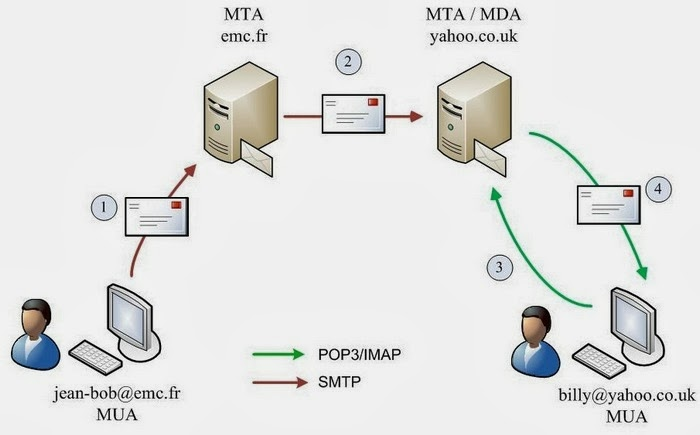
\includegraphics[width=1\textwidth]{Figures/mail_architektur.jpg}
	\caption{Here you insert the caption of the figure}
	\label{fig:mail_architektur}
\end{figure}

\noindent Die Struktur des E-Mail Verkehrs entspricht einer Client-Server Architektur und ist in Abbildung \ref{fig:mail_architektur} zu erkennen. Der Client, auch \acrfull{mua} genannt, bietet Möglichkeiten zum Verfassen, Versenden, Empfangen und Verwalten von E-Mails \citep[S. 142 f.]{Kurose2014}. Zum Versand wird das \acrfull{smtp} auf Port 25 (bzw. 587 verschlüsselt) verwendet. \acrshort{smtp} ist ein Protokoll zum Austausch von E-Mails in Netzwerken, verortet auf der Anwendungsschicht im \acrshort{osi}-Modell \citep[S. 4 ff.]{RFC5321}. In einer SMTP-Sitzung werden verschiedene Texte und Statuscodes verwendet, mit denen der MUA mit dem Mailserver, auch \acrfull{mta} kommunizieren kann. 

Zu Beginn der Session kündigt der Client sich mit dem Befehl \texttt{HELO} \texttt{servername.domain.tld} an. Der Server antwortet im Erfolgsfall stets mit dem Statuscode \texttt{250 OK}. Darauf gibt der Client jeweils den Absender mit \texttt{MAIL FROM:<absender@domain.tld>} und den Empfänger mit \texttt{RCPT TO:<empfaenger@domain.tld>} an. Zur Übertragung des Nachrichteninhalts wird \texttt{DATA} an den Server gesendet, als Antwort erhält der Client \texttt{354 start mail input} zurück. Nun kann der Client den Inhalt an den Server senden, das Ende wird hierbei durch eine Leerzeile mit einem Punkt folgend dargestellt. Der Server bestätigt erneut mit \texttt{250 OK}, worauf der Client die Verbindung mit \texttt{QUIT} beendet. Der Server quittiert dies zuletzt mit dem Statuscode \texttt{211 closing channel}. Tabelle \ref{tab:smtpversand} zeigt einen beispielhaften Versand einer E-Mail über SMTP von Client zu Server. \citep[S. 4 ff.]{RFC821}

Der Mailserver des Absenders sendet die Nachricht daraufhin an den Mailclient des Empfängers über \acrshort{smtp} weiter. Auch hierbei entspricht der Versand dem in Tabelle \ref{tab:smtpversand} sichtbaren Schema. Der \acrshort{mta} des Empfängers, auch \acrfull{mda} genannt, hält die E-Mail im Postfach des Empfängers vor, bis sich dieser mit seinem Mailserver verbindet. Es ist zu beachten, dass der Empfänger zur Verbindung \glqq[...] kein SMTP verwenden kann, um die Nachrichten zu erhalten, weil das Abrufen der Nachrichten eine Pull-Operation ist, während SMTP ein Push-Protokoll ist\grqq{} \citep[S. 150]{Kurose2014}.

\begin{table}[ht]
\centering
\caption[Beispiel: SMTP-Versand einer E-Mail]{Beispielversand einer E-Mail über SMTP}
\begin{tabular}{|l|l|}
\hline
\textbf{Client}                                                                                                                                                                                                                           & \textbf{Server}      \\ \hline
\texttt{HELO smtp.eme.fr}                                                                                                                                                                                                                          & \texttt{250 OK}               \\ \hline
\texttt{MAIL FROM:jean-bob@eme.fr}                                                                                                                                                                                                                 & \texttt{250 OK}               \\ \hline
\texttt{RCPT TO:billy@yahoo.co.uk}                                                                                                                                                                                                                 & \texttt{250 OK}              \\ \hline
\texttt{DATA}                                                                                                                                                                                                                                    & \texttt{354 start mail input} \\ \hline
\begin{tabular}[c]{@{}l@{}}From: \textless{}jean-bob@eme.fr\textgreater\\ To: \textless{}billy@yahoo.co.uk\textgreater\\ Subject: Cake\\ Date: Thu, 7 Apr 2022 16:26:49 +0200\\ \\ Hello Billy, how do you like my cake?\\ .\end{tabular} & \texttt{250 OK}              \\ \hline
\texttt{QUIT}                                                                                                                                                                                                                                      & \texttt{211 closing channel}  \\ \hline
\end{tabular}
\label{tab:smtpversand}
\end{table}

\noindent Aus diesem Grund wurden das \acrfull{pop3} und das \acrfull{imap} entworfen, welche \acrshort{mua}s den Abruf von E-Mails ermöglichen. \acrshort{pop3} kommuniziert über Port 110 (bzw. 995 verschlüsselt) und besitzt nur eingeschränkte Funktionen. Nach einem Verbindungsaufbau werden drei Phasen durchlaufen: Autorisierung, Transaktion und Aktualisierung. Zur Autorisierung überträgt der Client jeweils seinen User mit \texttt{USER} und sein Passwort mit \texttt{PASS} im Klartext und erhält bei erfolgreicher Autorisierung \texttt{+OK} als Statusmeldung zurück. In der Transaktionsphase kann der Client den Status des Postfachs mit \texttt{STAT}, eine Liste der E-Mails mit Größe mit \texttt{LIST} und den Inhalt einzelner E-Mails mit \texttt{RETR} abrufen. Bei letztem Befehl wird die Nummer der E-Mail im Postfach mit angegeben, die beim Aufruf von \texttt{LIST} angezeigt wird. Mit der selbigen Nummer ist es auch möglich E-Mails vom Server zu löschen indem man \texttt{DELE} nutzt. Hierbei wird das Löschen nicht direkt ausgeführt. Stattdessen beendet der Client die Sitzung mit \texttt{QUIT}, woraufhin die Aktualisierungsphase gestartet und alle \texttt{DELE}-Befehle ausgeführt werden. Um Löschungen vor Sitzungsende abzubrechen, kann \texttt{RSET} verwendet werden. Der beispielhafte Abruf der E-Mail aus Tabelle \ref{tab:smtpversand} ist in Tabelle \ref{tab:pop3abruf} zu sehen. \citep[S. 3 ff.]{RFC1939}


\begin{table}[ht]
\centering
\caption[Beispiel: POP3-Abruf einer E-Mail]{Beispielabruf der E-Mail aus Tabelle \ref{tab:smtpversand} mit POP3}
\begin{tabular}{|l|l|}
\hline
\textbf{Client} & \textbf{Server}                                                                                                                                                                                                                      \\ \hline
\texttt{USER billy@yahoo.co.uk}            & \texttt{+OK}                                                                                                                                                                                                                                  \\ \hline
\texttt{PASS secret-passwort}          & \texttt{+OK}                                                                                                                                                                                                                                  \\ \hline
\texttt{LIST}            & \begin{tabular}[c]{@{}l@{}}\texttt{+OK 1 37}\\ \texttt{+OK 2 534}\end{tabular}                                                                                                                                                                        \\ \hline
\texttt{RETR 1}          & \begin{tabular}[c]{@{}l@{}}From: \textless{}jean-bob@eme.fr\textgreater\\ To: \textless{}billy@yahoo.co.uk\textgreater\\ Subject: Cake\\ Date: Thu, 7 Apr 16:26:49 +0200\\ \\ Hello Billy, how do you like my cake?\\ .\end{tabular} \\ \hline
\texttt{DELE 1}          & \texttt{+OK}                                                                                                                                                                                                                                  \\ \hline
\texttt{QUIT}            & \texttt{+OK}                                                                                                                                                                                                                                  \\ \hline
\end{tabular}
\label{tab:pop3abruf}
\end{table}

Da \acrshort{pop3} E-Mails lediglich abrufen und löschen kann, wurde \acrshort{imap} entworfen, welches die Funktionalitäten \acrshort{pop3} erweitert und dadurch die Komplexität des Abrufs erhöht. \acrshort{imap} bietet die Möglichkeit verschiedene Ordner zu erstellen und zu verwalten, darüber hinaus können E-Mails in einer gekürzten Form abgerufen werden. Letzteres ist insbesondere bei Clients mit schwacher Internetverbindung hilfreich, da der Nutzer einen Überblick enthält und sich dann entscheiden kann, welche Nachricht er laden will. \citep[S. 2 ff.]{RFC3501}


\begin{table}[]
\centering
\caption[Beispiel: IMAP-Abruf einer E-Mail]{Beispielabruf der E-Mail aus Tabelle \ref{tab:smtpversand} mit IMAP}
\begin{tabular}{|l|l|}
\hline
\textbf{Client}                             & \textbf{Server}                                                                                                                                                                                                                                 \\ \hline
\texttt{a001 LOGIN billy secret-passwort}            & \texttt{a001 OK LOGIN}                                                                                                                                                                                                                                   \\ \hline
\texttt{a002 SELECT INBOX}                           & \begin{tabular}[c]{@{}l@{}}* \texttt{2 EXISTS}\\ * \texttt{FLAGS} \texttt{(\textbackslash{}Answered \textbackslash{}Deleted \textbackslash{}Seen)}\\ * \texttt{OK {[}UNSEEN 1{]}}\\ \texttt{a002 OK {[}READ-WRITE{]} SELECT}\end{tabular}      \\ \hline
\texttt{a004 FETCH 1 BODY{[}HEADER{]}}               & \begin{tabular}[c]{@{}l@{}}* \texttt{1 FETCH (BODY{[}HEADER{]}}\\   From: \textless{}jean-bob@eme.fr\textgreater\\   To: \textless{}billy@yahoo.co.uk\textgreater\\   Subject: Cake\\   Date: Thu, 7 Apr 16:26:49 +0200\\ \texttt{)}\\ \texttt{a004 OK FETCH}\end{tabular} \\ \hline
\texttt{a005 FETCH 1 BODY{[}TEXT{]}}                 & \begin{tabular}[c]{@{}l@{}}* \texttt{1 FETCH (BODY{[}TEXT{]}}\\   Hello Billy, how do you like my cake?\\ \texttt{)}\\ \texttt{a005 OK FETCH}\end{tabular}                                                                                                                 \\ \hline
\texttt{a006 STORE 1 +FLAGS \textbackslash{}Deleted} & \texttt{a006 OK +FLAGS}                                                                                                                                                                                                                                  \\ \hline
\texttt{a007 EXPUNGE}                                & \begin{tabular}[c]{@{}l@{}}* \texttt{1 EXPUNGE}\\ \texttt{a007 OK EXPUNGE}\end{tabular}                                                                                                                                                                           \\ \hline
\texttt{a008 LOGOUT}                                 & \texttt{a008 OK LOGOUT}  \\ \hline
\end{tabular}
\label{tab:imapabruf}
\end{table}

Tabelle \ref{tab:imapabruf} zeigt den Abruf der E-Mail aus Tabelle \ref{tab:smtpversand}. Zum Verbindungsaufbau wird der Befehl \texttt{LOGIN} mit User und Passwort in Klartext verwendet. Der Server antwortet mit \texttt{OK}, gefolgt vom Befehlsnamen, in diesem Fall \texttt{OK LOGIN}. Hierbei besitzt jeder Befehl ein vorangehendes Tag, anhand welchem sich ein Befehl zuordnen lässt, beispielsweise \texttt{a001}, \texttt{a002}... \citep[S. 6 f.]{RFC3501}. Nach erfolgreicher Autorisierung kann Client verschiedene Ordner öffnen, zum Beispiel den Posteingang mit \texttt{SELECT INBOX}. Er erhält sowohl ein \texttt{OK} vom Server, als auch eine Liste der im Ordner liegenden E-Mails, die erste ungelesene E-Mail, sowie die verfügbaren Flags, die die E-Mails weiter klassifizieren. Ähnlich zu \texttt{RETR} kann mit \texttt{FETCH} der Inhalt einer E-Mail angezeigt werden. Hierbei können sowohl der Nachrichten-Header als auch der Payload angezeigt werden mit \texttt{FETCH BODY[HEADER]}, bzw. \texttt{FETCH BODY[TEXT]}. Der Aufbau einer E-Mail wird nachfolgend detaillierter erläutert. Zum Löschen wird \texttt{STORE +FLAGS \textbackslash Deleted} ausgeführt, wodurch eine Nachricht entsprechend markiert wird. Um diese Nachrichten zu entfernen, wird \texttt{EXPUNGE} verwendet. Hierbei werden markierte Nachrichten permanent gelöscht. Abschließend kann der Client die Verbindung mit \texttt{LOGOUT} trennen. \citep[S. 2 ff.]{RFC3501}

Das zuvor beschriebene Szenario deckt jedoch nur den Erfolgsfall ab. Es ist jedoch möglich, dass ein Mailserver nicht erreichbar ist. Ist der \acrshort{mta} des Absenders nicht erreichbar, hält der \acrshort{mua} die Nachricht in einer Warteschlange vor und versucht sie erneut zu versenden. Selbiges gilt für einen \acrshort{mta}, der versucht die Nachricht an den \acrshort{mda} weiterzuleiten. Kann die Nachricht nach wiederholten Versuchen in festlegten Intervallen nicht versendet werden, wird sie aus der Nachrichtenwarteschlange entfernt und der Absender wird über den Vorgang informiert \citep[S. 144 f.]{Kurose2014}. Bei den Abrufprotokollen \acrshort{pop3} und \acrshort{imap} wird der Nutzer direkt informiert, wenn sein \acrshort{mda} nicht verfügbar ist, wiederholte Versuche müssen selbst initiiert werden.

E-Mails besitzen ein bestimmtes Format, welches in \acrshort{rfc} 5322 definiert wurde. Unterteilt wird in einen Header, der alle notwendigen Metainformationen enthält, und einen Body, der den eigentlichen Nachrichteninhalt enthält \citep[S. 6 ff.]{RFC5322}. Dabei sind Header und Body von einer Leerzeile getrennt, um sie auseinander zu halten. Zeile 6 in Tabelle \ref{tab:smtpversand} zeigt ein entsprechendes Beispiel. Verpflichtend sind dabei lediglich der Absender, mit \texttt{From:} spezifiziert, der Empfänger, mit \texttt{To:} spezifiziert und das Datum der Nachricht, mit \texttt{Date:} spezifiziert \citep[S. 18]{RFC5322}. Darüber hinaus existieren weitere standardisierte Header-Felder, wie z.B. \texttt{Priority} für die Priorität einer E-Mail.  Es ist außerdem möglich eigene Header zu setzen, wenn diese mit einem \texttt{X-} beginnen \citep[S. 24]{RFC822}. 

Für Header und Body stehen in der Ursprungsform der E-Mail lediglich 7-Bit \acrshort{ascii}-Zeichen zur Verfügung. Um diese Beschränkungen aufzuheben, wurden in \acrshort{rfc} 2045 Erweiterungen, \acrfull{mime} genannt, eingeführt. \acrshort{mime} bieten die Möglichkeit verschiedene Zeichensätze zu verwenden, indem diese in \acrshort{ascii} umkodiert werden \citep[S. 3 f.]{RFC2045}. Hierzu werden drei neue Headerfelder genutzt, welche die MIME-Version, den Inhaltstyp und die Kodierung definieren \citep[S. 9 f.]{RFC2045}. Diese Felder lauten \texttt{MIME-Version}, \texttt{Content-Type} und \texttt{Content-Transfer-Encoding}. Als MIME-Version wird 1.0 angegeben, als Content-Type können verschiedene Typen angegeben werden, die der jeweilige \acrshort{mua} selbst interpretiert. Mögliche Inhaltstypen sind unter anderem \texttt{text/plain} für einfachen Text, \texttt{text/html} für E-Mails im Markup-Format mit Styling, \texttt{image/png} für Bilder im \acrshort{png}-Format. Bei \acrshort{html} ist zu beachten, dass sich die Interpretation je nach \acrshort{mua} unterscheiden kann, wodurch unterschiedliche Darstellungen der selben Nachricht möglich sind \citep[S. 6 f.]{RFC2046}. Zum Versenden von Anhängen zusätzlich zu einer Nachricht wird \texttt{multipart/mixed} angegeben, wobei die einzelnen Anhänge durch einen \texttt{boundary}-Eintrag voneinander getrennt werden. Diese Einträge enthalten jeweils einen eigenen \texttt{Content-Type} und können weitere Informationen wie einen Dateinamen enthalten \citep[S. 268 f.]{Zisler2014}. 

Zuvor wurde bereits erläutert, wie ein Absender informiert wird, wenn seine Nachricht nicht an den \acrshort{mda} des Empfängers weitergeleitet werden kann. Es ist jedoch auch möglich eine Zustellbestätigung zu erhalten. Sowohl die Bestätigung über eine erfolgreiche als auch eine fehlgeschlagene Zustellung wird \acrfull{dsn} genannt. Diese werden über \acrshort{smtp} versendet, wobei als Absender \texttt{MAILER-DAEMON@domain.tld} und als Empfänger \texttt{<>} im Header angegeben wird \citep[S. 19 ff.]{RFC3461}. Zusätzlich wird über das Feld \texttt{Diagnostic-Code} ein Statuscode zurückgegeben, wie z.B. \texttt{5.2.2} bei einem vollen Posteingang des Empfängers oder \texttt{5.3.4} bei einer Nachricht, die zu groß für einen Mailserver ist \citep[S. 7 ff.]{RFC3463}. Da die Zustellbestätigung lediglich den Erhalt der E-Mail des \acrshort{mda} zusichert, wurden mit RFC 8098 und RFC 3503 Empfangsbestätigungen, auch \acrfull{mdn} genannt, eingeführt. Diese Bestätigungen werden vom jeweiligen \acrshort{mua} über \acrshort{pop3} oder \acrshort{imap} versendet, wenn er eine E-Mail erhalten hat \citep[S. 3 f.]{RFC3503}. Ob diese auch vom Empfänger gelesen wurde, ist dabei irrelevant \citep[S. 30 f.]{RFC8098}.

Ein großes Problem von E-Mails stellt die Sicherheit dar. So übertragen die vorgestellten Protokolle sowohl die Nachrichten als auch die Nutzeranmeldedaten im Klartext. Um letzteres abzusichern, kann das \acrfull{tls} Protokoll verwendet werden. Mit \acrshort{tls} können Daten im Internet verschlüsselt übertragen werden, wobei der Diffie-Hellman-Schlüsselaustausch verwendet wird, welcher private und öffentliche Schlüsselpaare kombiniert \citep[S. 95 f.]{RFC8446}. Um den Nachrichteninhalt selbst zu verschlüsseln oder zu signieren, bieten sich \acrfull{smime} an. Hierzu benötigen Empfänger ein von einer \acrfull{ca} ausgestelltes Zertifikat in Verbindung mit einem privaten Schlüssel; Absender benötigen zudem das Zertifikat des Empfängers \citep[S. 5 ff.]{RFC8551}. Mit diesen Informationen kann ein Absender eine E-Mail verschlüsseln und/oder signieren. Hierzu wird der Content-Type \texttt{multipart/signed} verwendet, wobei der erste Teil den Nachrichteninhalt und der zweite Teil Informationen zur Signatur in einer .p7s-Datei enthält \citep[S. 30 ff.]{RFC8551}. Mit Hilfe dessen kann der Empfänger die Echtheit und Authentizität der Nachricht prüfen. Aufgrund des mit diesem Verfahren verbundenen Aufwandes (Beschaffung eines Zertifikats bei einer \acrshort{ca}), wird \acrshort{smime} bei privaten Nutzern wenig verwendet, während es in Unternehmen häufig zu internen Signierung und Verschlüsselung angewendet wird \citep[S. 266]{Kappes2013}.


%----------------------------------------------------------------------------------------

\section{Bezahlsysteme zur Schaffung von Vorteilen in Videospielen (Pay to Win)}
\label{Bezahlsysteme_zur_Schaffung_von_Vorteilen_in_Videospielen_(Pay_to_Win)}

Die Priorisierung von E-Mails mittels eines Gegenwertes ähnelt dem Prinzip von Bezahlsystemen zur Schaffung von Vorteilen in Videospielen, auch Pay to Win oder Pay2Win genannt. Pay to Win beschreibt die Monetarisierung von Videospielen, die kostenlos oder kostenpflichtig sind. Bei der Monetarisierung handelt es sich um Mikrotransaktionen, die innerhalb der Spielwelt geschehen und damit keine feste Grenze zum Spielgeschehen aufweisen \citep[S. 18]{Tomic2019}. Pay2Win grenzt sich dabei von anderen Mikrotransaktionen ab, da es einen direkten Einfluss auf den Erfolg des Spielers hat, wohingegen kaufbare kosmetische Elemente den Erfolg des Spielers nicht beeinflussen \citep[S. 124 f.]{Reza2019}. Besonders in kostenlosen Spielen, verstärkt im mobilen Bereich, wird Pay2Win verwendet um Umsatz zu erzeugen. Hierbei werden Spieler nach einer gewissen Spielzeit kostenpflichtige Objekte und Aktionen angeboten, um ihren Fortschritt zu verbessern. Der Vorteil dieses Vorgehens ist, dass das Preismodell auf jeden Nutzer individuell zugeschnitten werden kann, was die Wahrscheinlichkeit einer Transaktion erhöht \citep[S. 2]{Alha2014}.

Grundsätzlich können zwischen drei Arten von Transaktionen unterschieden werden. So können gewisse Objekte in einem Spiel durch eine einmalige Zahlung erworben werden und bleiben dauerhaft im Besitz des Spielers. Hierbei handelt es sich nur um Pay2Win, wenn die Objekte dem Spieler einen Vorteil verschaffen. Eine weitere Art der Transaktionen sind Abonnements, bei denen Spieler einen temporären Vorteil erkaufen, der nur für die Zeit des Abonnements gilt. Die am weitesten verbreitete Art der Transaktion sind sogenannte Lootboxen. Lootboxen sind Pakete, welche Spieler kaufen können, um neue Objekte zu erhalten, wobei sie nicht wissen welche Objekte sie erhalten und welchen Wert diese widerspiegeln \citep[S. 20]{Tomic2019}. Spieler haben dabei keinen Einfluss auf den Inhalt von Lootboxen.

Die Effekte von Pay2Win unterscheiden sich je nach Art des Spiels. So dienen Transaktionen in einem Einzelspieler-Modus dem individuellen Fortschritt, beziehungsweise der Erleichterung des Spielers. In Mehrspieler-Modi hingegen erzeugt Pay2Win eine Ungleichheit zwischen Spielern, da die Zahlenden bevorzugt werden. Während diese Mechanik anfangs nur in kostenlosen Spielen auftrat, wird sie mittlerweile auch verstärkt in Titeln angewendet, die ohnehin kostenpflichtig sind \citep[S. 19]{Tomic2019}.

Die Definition eines Pay2Win-Spiels ist nicht klar definiert und von subjektiven Bewertungen geprägt. Aus diesem Grund versuchen \cite{Tregel2020} in einer Befragung Kriterien zu erarbeiten, welche ein Spiel als Pay2Win deklarieren. Es wurden 13 Kriterien erarbeitet, von denen fünf eine Zustimmung von über 2/3 der Befragten erhielten. Ein Spiel kann als Pay2Win erachtet werden, wenn es ab einem Punkt kaum/nicht mehr möglich ist es ohne Zahlung fortzuführen oder Fortschritt zu erlangen. Außerdem wurden Objekte, die einen Vorteil verschaffen und nur mit Echtgeld gekauft werden können, aufgeführt. Dies ist insbesondere ein Indikator von Pay2Win, wenn diese Objekte einen permanenten Vorteil verschafften oder in einem Mehrspieler-Modus hilfreich sind \citep[S. 179]{Tregel2020}. Diese Kriterien müssen nicht alle auf ein Spiel zutreffen, um als Pay2Win zu gelten.

Der größte Kritikpunkt an Pay2Win ist, abgesehen von der bereits erwähnten Privilegierung, der Einfluss, den Mikrotransaktionen auf Spieler haben. Insbesondere bei Lootboxen, deren Inhalt für den Spieler nicht vorhersehbar ist, finden sich Parallelen zum Glücksspiel. Da das eigene Geld meist in spielinterne Währung umgetauscht werden muss, deren Wechselkurs nicht transparent dargestellt wird, können Lootboxen mit Glücksspiel in Kasinos verglichen werden, in denen Chips o.ä. gekauft werden müssen, um teilzunehmen (\cite[S. 7 ff.]{Drummond2018},, \cite[S. 185 ff.]{Nielsen2019}). Da die Lootboxen direkt in das Spielgeschehen integriert werden, werden die Zahlungen von den Spielern seltener hinterfragt. Das führt insbesondere dazu, dass Menschen, die ein höheres Risiko haben von Glücksspiel abhängig zu werden, auch größere Summen in Lootboxen investieren \citep[S. 5 f.]{Zendle2018}. Darüber hinaus können auch Minderjährige, die keinen Zugang zu konventionellem Glücksspiel haben und tendenziell anfällig für jenes sind, Lootboxen kaufen. Dieser Umstand wird dadurch deutlicher, dass ein Großteil des Einkommens der Spieleentwickler durch Lootboxen von einer kleinen Spielergruppe kommt (\cite[S. 8 f.]{Zendle2020},, \cite{Takahashi2014}). Diese Spieler sind oft nicht in der finanziellen Position ihre Käufe zu tätigen und fallen den Mechaniken von Pay2Win zum Opfer \citep{Close2021}. Ein weiterer Indikator dafür, dass Lootboxen mit Glücksspiel verglichen werden können, sind die Verhaltensweisen von Spielern, die sich mit Glücksspielern überschneiden. So fanden verschiedene Studien heraus, dass Käufer von Lootboxen ihr eigentliches Budget überschreiten, um einen Einsatz zurück zu gewinnen; ein Indikator für mal-adaptives Verhalten (\cite[S. 9 ff.]{Nielsen2019},, \cite[S. 1968 f.]{King2018a},, \cite[S. 4 f.]{Xiao2021}).

Um die Problematik von Pay2Win und insbesondere ihre Auswirkungen hinsichtlich Spielsucht und ethischer Aspekte abzumildern, schlagen \cite{King2018} verschiedene Maßnahmen vor, die mit sozialer Verantwortung der Softwareentwickler einhergehen. Diese Maßnahmen sind in vier Kategorien verortet, die im Folgenden erläutert werden. Die erste Kategorie beschäftigt sich mit dem Design und dem Prozess von Mikrotransaktionen in Spielen. Hierbei wird die Art und Weise wie Objekte gekauft werden können adressiert. So sollen Spieler Preise stets in echter Währung einsehen können und ein Limit setzen, wie viel Geld sie in einem bestimmten Zeitraum ausgeben wollen. Außerdem soll der Zahlungsprozess durch Pausen und das Eingeben der Anmeldedaten verlangsamt werden, sodass Spieler reflektieren können, ob sie ein Objekt wirklich kaufen wollen. Lootboxen sollen außerdem nur Objekte enthalten, die Spieler auch innerhalb des Spiels erhalten können, zudem dürfen diese nicht ablaufen. Die Privilegierung von Spielern soll ebenfalls nicht möglich sein, sodass eine gewisse Fairness in Mehrspieler-Modi gewährleistet ist. Zudem darf der Kauf von Lootboxen nicht künstlich hervorgehoben werden durch zeitlich begrenzte Angebote, besondere Animationen oder andere Einfluss nehmende Strategien. Die zweite Kategorie behandelt die Transparenz von Features. Hierbei sind Entwickler angehalten Lootboxen als Teil des Spiels schon beim Verkauf zu deklarieren und die Chancen zum Erwerb von gewissen Objekten in Lootboxen zu kommunizieren. Als dritte Kategorie wird der Verbraucherschutz angeführt. Spiele mit Lootboxen, bzw. der Kauf von Lootboxen soll mit einer Altersbeschränkungen versehen werden. Außerdem sollen Spieler ihre bisherigen Zahlungen einsehen und limitieren können, analog zu Sportwetten. Eine Checkliste für die problematisches Verhalten soll Spielern helfen ihren Umgang mit Lootboxen zu bewerten. Zuletzt befasst sich die Kategorie der Verbraucherinformation und Industrieverantwortung mit der Informationen über Änderungen am Pay2Win-System, sowie der proaktiven Information der Spieler zu gesundem Glücksspiel \citep[S. 169 ff.]{King2018}. Auch wenn diese Vorschläge die Mechanik von Pay2Win spielerfreundlicher und sicherer machen würden, kann nicht davon ausgegangen werden, dass sie implementiert werden, wenn es keine Verpflichtung, beispielsweise durch den Gesetzgeber, gibt.

Als Beispiel für den Einsatz von Pay2Win eignet sich der Spielmodus \textit{FIFA Ultimate Team} der Spielreihe \textit{FIFA} von EA Sports. In diesem Mehrspieler-Modus stellen Spieler eine eigene Mannschaft aus Fußballprofis zusammen. Diese Profis haben dabei verschiedene Attribute, wie z.B. \textit{Sprintgeschwindigkeit} oder \textit{Schusskraft}, die mit Werten von 1 bis 100 beschrieben werden. Je höher ein Attribut ist, desto besser ist der Profi. Spieler können in Turnieren und Ligen Münzen gewinnen, mit welchen sie Profis auf Auktionen kaufen können. Zusätzlich gibt es die Möglichkeit Pakete zu kaufen, in denen sich, analog zu Sammelkarten, Profis befinden können, wobei der Spieler nicht weiß, welche Profis er erhält. Diese Pakete können ebenfalls mit Echtgeld gekauft werden und erfüllen somit die Kriterien für eine Lootbox. Hierbei werden die Pakete nicht direkt gekauft, stattdessen wird das Geld in sogenannte \textit{FIFA Points} umgewandelt, mit welchen man wiederum die Lootboxen kaufen kann. Zwar ist es auch möglich Pakete mit Münzen zu kaufen, in der Regel spiegelt der Aufwand für den Spieler den Ertrag des Paketes nicht wieder \citep[S. 188]{Tregel2020}. So wurden für das Finalturnier der FIFA eSports Meisterschaften 2019 ca. 27.000\$ benötigt, um mit Pay2Win ein ausreichendes Team zu stellen \citep{Akerman2019}. 
%!TEX root = ../main.tex
% Chapter 5

\chapter{Definition von Nutzeranforderungen}
\label{Definition_von_Nutzeranforderungen}

Nachfolgend werden die in Kapitel \ref{Operative_Ziele} definierten operativen Ziele in Nutzeranforderungen überführt. Darüber hinaus werden aus den Interessen, Ansprüchen, Anteilen und Anrechten der Stakeholder aus Kapitel \ref{Stakeholderanalyse} weitere Anforderungen definiert. Die Anforderungen werden im User Story Format von \cite{Cohn2004} formuliert und beinhalten eine Beschreibung aus Nutzersicht, eine Erklärung des Zwecks, sowie eine darauf folgende Liste an Akzeptanzkriterien. Darüber hinaus wird die Priorität mit 1 (niedrig) bis 3 (hoch) angegeben. Die Anforderungen dienen als Basis für die technische und inhaltliche Konzeption, sowie die spätere Implementation des Systems.


%----------------------------------------------------------------------------------------

\section{Anforderungen von Absendern}
\label{Anforderungen_von_Absendern}

\textbf{Einsicht des Nachrichtenaufkommens beim Empfänger} \\
Priorität: 1 \\
Als Absender möchte ich die Anzahl der zu bearbeitenden E-Mails beim Empfänger einsehen können, um einzuschätzen wie lange ich auf eine potenzielle Antwort warten muss.
\begin{itemize}
    \item Die Anzahl der offenen Nachrichten ist dem Absender bekannt und kann eingesehen werden.
    \item Persönliche Daten und Informationen werden dem Absender nicht übermittelt.
    \item Die voraussichtliche Antwortzeit, abhängig von der Bearbeitungsleistung (s.u.) des Empfängers, wird angezeigt.
\end{itemize}

\noindent
\\ \textbf{Priorisierbarkeit von E-Mails mit Gegenwert} \\
Priorität: 1 \\
Als Absender möchte ich eine E-Mail mit einem endlichen Gegenwert versehen können, um eine schnellere Bearbeitung gewährleistet zu bekommen.
\begin{itemize}
    \item E-Mails können optional mit einem Gegenwert versehen werden, der für Absender und Empfänger einsehbar ist.
    \item Dem Gegenwert wird eine Bearbeitungszeit zugeordnet, die von Absender und Empfänger einsehbar ist.
    \item Die Bearbeitungszeit ist verbindlich und muss berücksichtigt werden.
\end{itemize}

\noindent 
\textbf{Technologisch unabhängige Nutzung} \\
Priorität: 2 \\
Als Absender möchte ich meinen bevorzugten E-Mail Client verwenden können, um technologisch flexibel zu sein.
\begin{itemize}
    \item Die Einsicht in das Nachrichtenaufkommen und die Priorisierung von E-Mails sind clientunabhängig und können von jeglichem Endgerät aus genutzt werden.
    \item Die Priorisierung wird unmittelbar im E-Mail Standard umgesetzt.
    \item Die zusätzlich nötige Implementation kann von jedem Client ohne weitere Schritte eingebunden werden.
\end{itemize}

\noindent 
\\ \textbf{Sicherheit der E-Mails und Zahlungen} \\
Priorität: 2 \\
Als Absender möchte ich meine E-Mails, sowie Zahlungsinformationen sicher übertragen um Missbrauch zu verhindern.
\begin{itemize}
    \item Der Inhalt von E-Mails, sowie Informationen über das Nachrichtenaufkommen werden verschlüsselt übertragen und sind von außen nicht einsehbar.
    \item Zahlungsvorgänge und -informationen werden verschlüsselt übertragen und sind von außen nicht einsehbar.
\end{itemize}

\noindent 
\\ \textbf{Keine Verlangsamung des E-Mail Prozesses} \\
Priorität: 3 \\
Als Absender möchte ich meine aktuelle Geschwindigkeit beim E-Mail Versand beibehalten, um meine Produktivität nicht einzuschränken.
\begin{itemize}
    \item Die Einsicht in das Nachrichtenaufkommen verlangsamt den Prozess des E-Mail Versands nicht signifikant.
    \item Die Priorisierung von E-Mails verlangsamt den Prozess des E-Mail Versands nicht signifikant.
\end{itemize}

%----------------------------------------------------------------------------------------

\section{Anforderungen von Empfängern}
\label{Anforderungen_von_Empfaengern}


\textbf{Automatische Triage von E-Mails} \\
Priorität: 1 \\
Als Empfänger möchte ich priorisierte E-Mails angezeigt und vor-sortiert erhalten, um meine persönliche Triage zu verkürzen.
\begin{itemize}
    \item Priorisierte E-Mails werden nach ihrem Gegenwert sortiert angezeigt.
    \item Priorisierten E-Mails wird ein Fälligkeitsdatum, abhängig von der eigenen Bearbeitungsleistung (s.u.), hinzugefügt, welches verbindlich ist.
    \item E-Mails ohne Gegenwert werden nicht sortiert und erhalten kein Fälligkeitsdatum.
\end{itemize}

\noindent
\\ \textbf{Definition der Bearbeitungsleistung} \\
Priorität: 2 \\
Als Empfänger möchte ich meine Bearbeitungsleistung hinterlegen können, um die Triage transparenter zu gestalten und Absender zu informieren.
\begin{itemize}
    \item Es kann eine Bearbeitungsleistung definiert werden, die die Anzahl der vom Empfänger zu bearbeitenden E-Mails pro Tag beschreibt.
    \item Die Bearbeitungsleistung ist für den Empfänger verbindlich und muss eingehalten werden.
    \item Eine Abweichung von der Bearbeitungsleistung und die damit entstehende Verzögerung wird dem Absender automatisch mitgeteilt.
\end{itemize}

\noindent
\\ \textbf{Integrität der E-Mails und Zahlungen} \\
Priorität: 2 \\
Als Empfänger möchte ich bei priorisierten E-Mails sichergehen können, dass der  Gegenwert auch tatsächlich hinterlegt wurde.
\begin{itemize}
    \item Der Gegenwert einer E-Mail kann nicht anhand ihres Headers oder Bodys von außen ausgelesen werden.
    \item Es ist nicht möglich Zahlungen zu fälschen oder den Gegenwert einer E-Mail zu verändern.
    \item Zahlungen sind an einer nicht kompromittierbaren Stelle gespeichert und werden beim Empfang von E-Mails abgeglichen.
\end{itemize}

\noindent
\\ \textbf{Abweichungen der automatischen Triage} \\
Priorität: 3 \\
Als Empfänger möchte ich E-Mails nachträglich sortieren und priorisieren können, um für mich relevante Nachrichten, die keinen Gegenwert erhalten haben, schneller bearbeiten zu können.
\begin{itemize}
    \item E-Mails können nach der Triage höher priorisiert werden, als sie es eigentlich sind.
    \item Es können Regeln definiert werden (z.B. anhand bestimmter Absender oder gewisser Begriffe im Betreff), anhand welcher E-Mails nach der eigentlichen Triage höher priorisiert werden.
    \item Von der Triage abweichende E-Mails erhalten kein Fälligkeitsdatum.
    \item Von der Triage abweichende E-Mails, die bearbeitet werden, werden nicht zur täglichen Bearbeitungsleistung hinzugezählt.
\end{itemize}

\section{Übergreifende Nutzeranforderungen}

\textbf{Erreichbarkeit} \\
Priorität: 1 \\
Als Nutzer möchte ich die Priorisierung und Einsicht jederzeit nutzen können, um sie verlässlich in meinen E-Mail Prozess zu integrieren.
\begin{itemize}
    \item Die Priorisierung und Einsicht sind jederzeit verfügbar.
    \item Bei Nichterreichbarkeit sind Alternativen formuliert, die zumindest einen Teil der o.g. Anforderungen erfüllen.
\end{itemize}

\noindent
\\ \textbf{Koexistenz zu bisherigen Kanälen} \\
Priorität: 2 \\
Als Nutzer möchte ich meine bisherigen Kommunikationskanäle weiter nutzen können, um unabhängig zu bleiben.
\begin{itemize}
    \item Kommunikationskanäle außerhalb der E-Mail bleiben unverändert.
    \item E-Mails können weiter im herkömmlichen Sinne verwendet werden, die Priorisierung ist optional.
\end{itemize}

\noindent
\\ \textbf{Intuitive Nutzung} \\
Priorität: 2 \\
Als Nutzer möchte eine der bisherigen E-Mail ähnlichen Oberfläche erhalten, um einen möglichst einfachen Übergang zu haben.
\begin{itemize}
    \item Die Benutzeroberfläche ähnelt bisherigen E-Mail Clients.
    \item Die Benutzeroberfläche ist einfach verständlich und bietet einen schnellen Umstieg.
    \item Es ist möglich seinen E-Mail Prozess ohne einen großen Aufwand umzustellen.
\end{itemize} 
%!TEX root = ../main.tex
% Chapter 6

\chapter{Recherche nach vergleichbaren Produkten und Forschungen}
\label{Recherche_nach_vergleichbaren_Produkten_und_Forschungen}

Das folgende Kapitel listet Produkte und Forschungsergebnisse auf, die die zuvor gestellten Anforderungen zumindest teilweise erfüllen. Aus dieser Recherche werden Features, Ansätze und Erkenntnisse abgeleitet, die als Basis für das zu entwickelnde System gelten.

\section{E-Mail Headerfeld für Priorität}
Ein erster Lösungsansatz wäre die Nutzung des E-Mails Headers zum Setzen der Priorität. Da dieses Feld bereits in diversen MUAs und bei Nutzern etabliert ist, müsste hierfür keine neue Technologie implementiert werden. Außerdem ist das Feld bereits im E-Mail Standard integriert. Auch ist es mit IMAP möglich E-Mails zuerst zu erhalten, die als priorisiert gekennzeichnet sind.

Der Ansatz bringt jedoch diverse Probleme mit sich. So wurde in Kapitel \ref{Kontext_und_Domaene} bereits erwähnt, dass das Feld von Empfängern in ihrer Triage häufig nicht berücksichtigt wird \citep[S. 279 f.]{Whittaker1996}. Darüber hinaus gibt es auch keine Konventionen, wann eine E-Mail eine höhere Priorität hat und wann nicht, da dies ein subjektives Empfinden ist. So müssten konsistente und verbindliche Standards definiert werden, nach welchen eine E-Mail priorisiert ist und damit schneller bearbeitet wird. Selbst mit diesen Standards könnten Absender eine E-Mail Warteschlange nicht gezielt steuern und haben keine Einsicht in die noch offenen E-Mails beim Empfänger.

\section{E-Mails manuell mit Gegenwert versehen}
Um eine gezieltere und verbindlichere Priorisierung zu ermöglichen, könnten E-Mails manuell mit einem Gegenwert versehen werden. So könnten Empfänger ihre Absender informieren, dass sie Zahlungen über gewisse Wege annehmen. Absender würden dann unabhängig vom Versand der E-Mail eine Zahlung hinterlegen und diese in der E-Mail selbst referenzieren. Der Empfänger müsste die Zahlungen mit seinem Postfach abgleichen, um eine Triage durchzuführen.

Ein solches Vorgehen würde zu einem immensen Aufwand für den Empfänger führen, da dieser nicht nur sein Postfach, sondern auch sein/e Zahlungskonto/-en abgleichen muss, bevor die Triage durchgeführt werden kann. Außerdem muss im Zweifel jede E-Mail geöffnet werden, um die Referenz zur Zahlung zu finden. Diese händische Arbeit birgt ein großes Fehlerpotenzial. Zudem kann dieses Verfahren nicht universell angewendet werden, da verschiedene Empfänger unter Umständen verschiedene Zahlungswege bevorzugen, die zeitverzögert sein können. Beispielsweise könnte so eine E-Mail mit einem hohen Zahlungsbetrag erst nach mehreren Werktagen bearbeitet werden, wenn der Empfänger eine zugehörige Überweisung abwarten muss. Auch muss die Sicherheit betrachtet werden. Personen können sich als der Empfänger einer E-Mail ausgeben und ihre Zahlungswege an Personen weiterleiten, ohne dass diese mit dem eigentlichen Empfänger in Verbindung stehen. So wäre es möglich Zahlungen fälschlicherweise abzugreifen.

\subsection{Onlineshops}
Um den Zahlungsprozess zu automatisieren, könnten Empfänger ein Shop-System einrichten. Hierbei kaufen sich Absender einen Platz in der Warteschlange des Empfängers und geben beim Kauf ihre Nachricht an. Hierdurch könnten menschliche Fehler und Kompromittierung eingegrenzt werden, allerdings würde ein solches Vorgehen individuell sein und sich vom E-Mail Standard distanzieren. Auch wäre die Aussagekraft eines gekauften Platzes recht gering, da z.B. 500 Personen gleichzeitig einen Platz kaufen könnten in der Erwartung, dass ihre E-Mail schnell bearbeitet wird, ohne zu wissen, dass das Aufkommen sehr hoch ist. Dieses Problem wäre mit einer begrenzten Verfügbarkeit an Plätzen zu lösen. Eine gezielte Absendersteuerung, sowie eine Einsicht in das Aufkommen des Empfängers würde hierbei jedoch nicht abgedeckt werden.

\subsection{Payment-Based Email}
\label{Payment-Based_Email}
\cite{Turner2003} beschäftigen sich in \textit{Payment-Based Email} mit der Monetarisierung von E-Mails. Im Vordergrund steht die Abwehr von Spam mit der Versendung von Zahlungen innerhalb der E-Mail. Konkret solle SMTP um den Befehl \texttt{PAYMENT} erweitert werden. Die Zahlungen sollen über das \acrfull{lcp}, einem Protokoll für leichtgewichtige organisationsspezifische Währungen, ablaufen. So kann ein Unternehmen eine interne Währung definieren und sie an ihre Mitglieder verteilen, sodass sie die Währung einer E-Mail hinzufügen, um die Authentizität sicherzustellen.

Ein Vorteil ist die direkte Integration in den E-Mail Standard, wodurch keine Drittanbieter wie Onlineshops genutzt werden müssten. Dadurch könnte Payment-Based Email direkt in MUAs genutzt werden und auch eine Priorisierung wäre mit geringen Anpassungen möglich. Die Nutzung von LCP gibt die Möglichkeit Absender mit einer gewissen Menge der Währung auszustatten, sodass Zahlungen mit Echtgeld nicht notwendig sind.

Das System sowie der PAYMENT-Befehl und LCP wurden zwar konzeptioniert, jedoch nie als RFC formuliert oder umgesetzt. Hinzu kommt, dass das Prinzip auf dem technologischen Stand von vor ca. 20 Jahren ist. Mittlerweile sind neue Zahlungsmechanismen wie Cryptowährungen im Umlauf, die LCP ersetzen können. Außerdem gibt es keinen Prozessschritt vor dem Setzen einer Zahlung, der es ermöglicht eine Einsicht in die Warteschlange zu erhalten. Ebenfalls wird die Bearbeitungsleistung des Empfängers nicht berücksichtigt, sodass Zahlungen keine verbindliche Bearbeitung erzeugen. \citep[S. 3 f.]{Turner2003}

%----------------------------------------------------------------------------------------

\section{Ticketsysteme und Helpdesks}
Während sich die vorangegangenen Konzepte insbesondere mit der Priorisierung von E-Mails, sowie Zahlungsmöglichkeiten beschäftigten, werden nun Warteschlangen und transparente Kommunikation an Absender thematisiert. Zur Koordination von IT-Supportanfragen werden in größeren Unternehmen Produkte wie \textit{JIRA Service Management}, \textit{Zendesk}, \textit{HappyFox}, \textit{Ivanti} oder \textit{Freshdesk} verwendet. Diese Produkte ermöglichen es aus Anfragen Tickets zu erzeugen, die sich in einer Warteschlange befinden und von verschiedenen Personen bearbeitet werden können. Die Tickets können über eine eigene Oberfläche, Website oder auch telefonisch oder per Mail generiert werden \citep{jiramail}. Auch ist es Bearbeitern möglich die Kommunikation ausschließlich via E-Mail zu führen. Es können verschiedene Prozesse automatisiert werden, so ist es beispielsweise möglich beim Erhalt einer E-Mail dem Absender eine Rückmeldung zu geben an welcher Position der Warteschlange er sich befindet und wie hoch die durchschnittliche Wartezeit ist. Auch können Personen priorisiert werden, deren Anfragen prinzipiell zuerst bearbeitet werden.

Während Ticketsysteme und Helpdesks somit eine hohe Transparenz hinsichtlich der Bearbeitungszeit und dem Aufkommen haben, ist eine Triage und Priorisierung nur schwer möglich. Die Priorisierung muss in einer manuellen Triage durchgeführt werden, alternativ dazu können Zahlungen, wie bereits erwähnt, unabhängig durchgeführt und verwaltet werden. Das Installieren und Betreiben eines eigenen Ticketsystems ist im Vergleich zum Aufsetzen eines E-Mail Kontos zeit- und kostenaufwändig, insbesondere bei technisch wenig versierten Anwendern.

%----------------------------------------------------------------------------------------

\section{Regeln zur automatischen Triage}
Während Ticketsystemen die Möglichkeit zur automatischen Triage fehlt, könnte diese in E-Mail Clients zumindest teilweise konfiguriert werden. Nutzer haben die Möglichkeit Regeln festzulegen nach welchen E-Mails gelöscht, mit einer Priorität versehen oder in verschiedene Ordner verschoben werden. Die Regeln können anhand verschiedener Parameter wie Absender, Betreff, Nachrichteninhalt, Nachrichtenlänge etc. definiert werden.

Zwar kann die Triage dadurch teil-automatisiert werden, jedoch ist der initiale Aufwand für solche Regeln sehr hoch, insbesondere wenn sie verlässlich und treffend funktionieren sollen. Außerdem müssen Regeln im Laufe der Zeit angepasst werden wenn sich wichtige Absender ändern oder ein bestimmtes Thema besonders relevant wird. Auch ist diese Form der Triage allein durch den Empfänger gesteuert und bietet weder Transparenz über das Aufkommen, noch eine Priorisierung durch Absender.

\subsection{Intelligente Systeme zur Triage}

Eine Erweiterung des Konzepts von Regeln stellen \cite{Koprinska2007} dar. In \textit{Learning to classify e-mail} wird das Ablegen von E-Mails in Ordnern, sowie die Filterung nach Spam mittels einer künstlichen Intelligenz durchgeführt, die das \textit{Random Forest}-Verfahren angewendet. Dieses Verfahren dient zur Klassifikation von Daten mittels Entscheidungsbäumen \citep[S. 5 f.]{Breiman2001}. Die Klassifikation erfolgt mit der Gewichtung verschiedener Faktoren des Datensatzes. Die Faktoren müssen jedoch vordefiniert werden, sodass das System trainiert werden kann. Somit können keine individuellen Faktoren definiert werden, was das System kaum nutzbar macht. Außerdem ist die Genauigkeit des Systems mit 81\% bis 96\% nicht ausreichend, um es als alleiniges Mittel zur Triage zu verwenden \citep[S. 2174]{Koprinska2007}. Da das System lediglich mit dem Sortieren in Ordnern und nicht mit einer wirklichen Priorisierung getestet wurde, ist es als Lösungsansatz zu vernachlässigen.

%----------------------------------------------------------------------------------------

\section{Erkenntnisse für das zu entwickelnde System}
\label{Erkenntnisse_fuer_das_zu_entwickelnde_System}
Die zuvor beschriebenen Produkte und Forschungsansätze bieten verschiedene Aspekte, die für das zu entwickelnde System aufgegriffen werden können. Grundsätzlich ist festzuhalten, dass kein Produkt/Ansatz die Anforderungen voll erfüllt oder die Forschungsfrage hinreichend beantwortet. Zwar wäre auch eine Kombination jener Produkte/Ansätze mittels verschiedener Schnittstellen möglich, allerdings wäre dies mit einem hohen Aufwand verbunden und hinsichtlich proprietärer Produkte oder einer späteren Weiterentwicklung nicht nachhaltig. Somit ist die Entwicklung eines neuen Systems erforderlich.

Der in \textit{Payment-Based Email} genannte Ansatz der integrierten Zahlungen kann hierbei als Basis dienen. Statt der Implementation eines neuen SMTP-Befehls kann ein individueller E-Mail Header verwendet werden. Das hat den Vorteil, dass sich kein neuer technischer Standard als RFC etablieren muss, sondern bisherige Technologien verwendet werden können. Die Zahlung muss demzufolge aus der E-Mail extrahiert werden, dadurch wird die Interoperabilität des Systems gewährleistet. 

Eine solche Extraktion ist über die Entwicklung einer eigenen Komponente zur Zahlungsabwicklung möglich, die das Ziel hat, ein Headerfeld mit Zahlungsinformationen zu erzeugen. Dieses Headerfeld kann von einem Empfängerclient ausgelesen und zur automatischen Triage verwendet werden. Konventionelle E-Mails ohne ein entsprechendes Feld können als niedriger priorisiert betrachtet und vom Client entsprechend angezeigt werden.

Somit kann der Absender in seinem bisherigen Client weiterhin E-Mails versenden, wenn die Zahlung extern abgewickelt wird. Die einzige Erweiterung des Absenderclients ist das Setzen des neuen Headerfelds. Komplexer gestaltet sich der Client des Empfängers; da dieser die Triage übernimmt, muss er eigens implementiert werden und kann nicht als Erweiterung eines bestehenden Clients fungieren. Auch da zur Nutzung des Systems grundlegende Konfigurationen, wie Zahlungswege und die eigene Bearbeitungsleistung, notwendig sind, ist die Implementation eines eigenen Clients unabdingbar.

Der Vorteil dieser Aufteilung ist, dass E-Mails weiter uneingeschränkt nutzbar sind und Absender nicht mit dem neuen System interagieren müssen, wenn sich nicht an einer Priorisierung interessiert sind. Die Einsicht in das Nachrichtenaufkommen des Empfängers kann im Zuge des Zahlungsmoduls geschehen. Beim Zahlungsmodul muss sichergestellt sein, dass Zahlungen sicher und un-kompromittierbar durchgeführt werden.

 
%!TEX root = ../main.tex
% Chapter 7

\chapter{Inhaltliche Konzeption des Systems}
\label{Inhaltliche_Konzeption_des_Systems}

Dieses Kapitel beschäftigt sich mit der inhaltlichen Konzeption des Systems, welches nachfolgend auch \textit{Pay2Mail} genannt wird. Der Fokus liegt auf der Interaktion des Nutzers mit dem System, organisatorischen Fragen, sowie einer Vorauswahl von Bezahl- und Tokensystemen, die in Kapitel \ref{Nutzerbefragung_zum Bezahl-_und_Tokensystem} zur Auswahl stehen.

\section{Auswahl von Bezahl- und Tokensystemen}
\label{Auswahl_von_Bezahl-_und_Tokensystemen}
In Kapitel \ref{Bezahlsysteme_zur_Schaffung_von_Vorteilen_in_Videospielen_(Pay_to_Win)} wurden verschiedene Zahlungsmodelle vorgestellt, mit denen in Videospielen ein Gegenwert erzeugt wird. Zu Beginn ist das Abonnement zu nennen, mit welchem ein Vorteil für einen Zeitraum unter der Voraussetzung der regelmäßigen Zahlungen erworben wird. Für Pay2Mail eignet sich dieser Ansatz nicht, da ein Abonnementspreis statisch wäre und sich nicht anhand des E-Mail Aufkommens verändert. Das bedeutet, dass eine E-Mail je nach Monat und Bearbeitungsleistung unterschiedliche Bearbeitungszeiten hätte, ohne dass Nutzer aktiv priorisieren könnten. Stattdessen kann nur eine generelle Tendenz zur Priorisierung gegeben werden, vergleichbar mit dem Express-Versand, den Logistikunternehmen anbieten. Ein weiterer Nachteil ist die fehlende Flexibilität. So eignet sich ein Abonnement nur für Nutzer, die einen kleinen Empfängerkreis haben, den sie häufig kontaktieren. Andernfalls müssten viele Abonnements abgeschlossen werden, was ineffizient und kostenaufwändig ist.

Statt eine laufendes Abonnement vorauszusetzen, könnten Zahlungen spezifisch pro E-Mail gesetzt werden. Der Vorteil ist, dass die Höhe abhängig vom Empfänger und dessen Aufkommen festgelegt werden kann. Außerdem ist, im Vergleich zu Abonnements, ein individueller Betrag setzbar, ohne dass eine Preisstaffelung erfolgt. Auch ist dieses Vorgehen in der automatischen Triage effektiver, da Zahlungen miteinander verglichen werden können, ohne dass gleich hohe Abonnementspreise den Empfänger zwingen eine eigene Triage durchzuführen. 

Ein Nachteil von Zahlungen mit Echtgeld ist, dass eine Benachteiligung von Personen entsteht, die sich solche Zahlungen nicht leisten können, obwohl E-Mails versenden müssen, die eine hohe Priorität haben. Das führt dazu, dass nicht relevante E-Mails priorisiert werden, sondern E-Mails von Personen, die sich eine Priorisierung leisten können. Dies ist insbesondere bei Empfängern mit einem sehr hohen Aufkommen oder geringer Bearbeitungsleistung der Fall. Um diese soziale Diskrepanz zu begleichen bieten sich token-basierte Gegenwerte an. Absender erhalten für einen fest definierten Zeitraum eine Anzahl an Token, welche sie als Gegenwert setzen können. Somit ist der finanzielle Stand eines Absenders irrelevant, vielmehr zählt wie er seine Token verwendet. Das Tokensystem ist dem Konzept des \acrshort{lcp} aus Kapitel \ref{Payment-Based_Email} nachempfunden. 

Ein Tokensystem löst zwar die soziale Ungleichheit in der Priorisierung von Absendern, sorgt allerdings auch dafür, dass Token nicht so verteilt sind, wie sie benötigt werden. Es gibt Absender, die eine größere Anzahl an E-Mails priorisiert versenden wollen, als es der durchschnittliche Absender würde. Solche Intensivnutzer hätten mit dem Tokensystem keine Möglichkeit ihr hohes Sendeaufkommen vollständig zu priorisieren. Absender mit wenigen E-Mails hingegen können eine unproportional große Anzahl an Token auf wenige E-Mails setzen und sich durch ihre geringe Nutzung einen Vorteil verschaffen. Eine Kombination aus Echtgeldzahlungen und Token würde dieses Problem lösen. Das bedeutet, dass jeder Nutzer eine spezifische Anzahl an \textit{Grundtoken} erhält, um E-Mails unabhängig von der eigenen finanziellen Situation priorisieren zu können. Nutzer mit vielen E-Mails können darüber hinaus weitere Token erwerben, um ihrem hohen Bedarf gerecht zu werden. Wichtig ist hierbei, dass die Token einen festen und unveränderlichen Preis haben. Dadurch können intransparente Preisstrukturen und kasino-ähnliche Verhaltensweisen, wie in Kapitel \ref{Bezahlsysteme_zur_Schaffung_von_Vorteilen_in_Videospielen_(Pay_to_Win)} erläutert, vermieden werden, was die Vertrauenswürdigkeit von Pay2Mail erhöht.

Somit werden den Befragten in Kapitel \ref{Nutzerbefragung_zum Bezahl-_und_Tokensystem} drei Bezahl- und Tokensysteme vorgeschlagen: Priorisierung von E-Mails mit Echtgeld; Setzen von Token, die jeder Nutzer in gleicher Menge erhält oder die Erweiterung dessen mit der Option Token mit Echtgeld nachzukaufen.

%----------------------------------------------------------------------------------------

\section{Use Cases}
\label{Use_Cases}
Im Folgenden werden Anwendungsfälle (Use Cases) definiert, die dazu dienen die Bedürfnisse des Nutzers, seine Interaktion, sowie seinen gewünschten Zielzustand festzuhalten.

\subsection*{Use Case 1: Priorisierung einer E-Mail}
\textbf{Akteur}: Absender einer E-Mail \\
\textbf{Vorbedingung}: Der Empfänger hat Pay2Mail konfiguriert und nutzt es aktiv. \\
\textbf{Auslöser}: Nutzer muss eine E-Mail versenden, die priorisiert bearbeitet werden soll. \\
\textbf{Endzustand im Erfolgsfall}: Nutzer hat die E-Mail mit einem Gegenwert versendet. \\
\textbf{Endzustand im Fehlerfall:} Nutzer konnte keinen Gegenwert an die E-Mail anhängen und hat sie unpriorisiert versendet. \\

\noindent \textbf{Normaler Ablauf}:
\begin{enumerate}
    \item Nutzer öffnet einen Mailclient seiner Wahl.
    \item Nutzer trägt den Empfänger der E-Mail ein.
    \item Nutzer erhält die Information zur möglichen Priorisierung.
    \item Nutzer öffnet die Oberfläche zur Priorisierung und zahlt einen Gegenwert.
    \item Nutzer erhält E-Mail Header zur Bestätigung der Zahlung.
    \item Nutzer setzt E-Mail Header und füllt die restlichen Felder aus.
    \item Nutzer versendet die E-Mail.
\end{enumerate}

\noindent \textbf{Erweiterungen}:
\begin{enumerate}
\setcounter{enumi}{3}
    \item a) Nutzer sieht sich vor der Zahlung das E-Mail Aufkommen an, um eine Entscheidung über die Höhe des Gegenwerts zu treffen.
\end{enumerate}

\noindent \textbf{Variationen}:
\begin{enumerate}
\setcounter{enumi}{5}
    \item \textquotesingle{} Nutzer setzt den Header nicht selbst, stattdessen wird er automatisch ausgefüllt.
\end{enumerate}


\subsection*{Use Case 2: Einsicht in das E-Mail Aufkommen eines Empfängers}
\textbf{Akteur}: Absender einer E-Mail \\
\textbf{Vorbedingung}: Der Empfänger hat Pay2Mail konfiguriert und nutzt es aktiv. \\
\textbf{Auslöser}: Nutzer ist interessiert daran, wie lange er auf eine Antwort warten muss. \\
\textbf{Endzustand im Erfolgsfall}: Nutzer kennt das E-Mail Aufkommen des Empfängers und die potenzielle Bearbeitungszeit. \\
\textbf{Endzustand im Fehlerfall:} Nutzer kann die potentielle Bearbeitungszeit nicht ermitteln. \\

\noindent \textbf{Normaler Ablauf}:
\begin{enumerate}
    \item Nutzer öffnet einen Mailclient seiner Wahl.
    \item Nutzer trägt den Empfänger der E-Mail ein.
    \item Nutzer erhält die Information zur möglichen Priorisierung.
    \item Nutzer öffnet die Oberfläche zur Priorisierung.
    \item Nutzer wählt die Auflistung des Aufkommens mit Bearbeitungszeit aus.
    \item Nutzer kann die Bearbeitungszeit je nach Gegenwert ablesen.
    \item Nutzer schließt die Oberfläche und den Mailclient.
\end{enumerate}

\noindent \textbf{Erweiterungen}:
\begin{enumerate}
\setcounter{enumi}{5}
    \item a) Nutzer zahlt einen Gegenwert, siehe ab Schritt 5 von Use Case 1.
\end{enumerate}

\noindent \textbf{Variationen}:
\begin{enumerate}
\setcounter{enumi}{4}
    \item \textquotesingle{} Nutzer sieht nicht die Bearbeitungszeit, sondern die Bearbeitungsleistung des Empfängers.
\end{enumerate}


\subsection*{Use Case 3: Automatische Triage des Posteingangs}
\textbf{Akteur}: Empfänger von E-Mails \\
\textbf{Vorbedingung}: Der Empfänger hat Pay2Mail konfiguriert. \\
\textbf{Auslöser}: Nutzer muss seine E-Mails bearbeiten und sein Postfach kontrollieren. \\
\textbf{Endzustand im Erfolgsfall}: Der Posteingang ist sortiert und der Nutzer weiß unmittelbar welche E-Mails er wann bearbeiten muss. \\
\textbf{Endzustand im Fehlerfall}: Der Posteingang ist unsortiert und der Nutzer muss die Triage selbst durchführen. 

\newpage

\noindent \textbf{Normaler Ablauf}:
\begin{enumerate}
    \item Nutzer öffnet die Anwendung.
    \item Nutzer sieht die zu bearbeitenden E-Mails in sortierter Form.
    \item Nutzer bearbeitet E-Mails entsprechend seiner Bearbeitungsleistung.
    \item Nutzer schließt die Anwendung.
\end{enumerate}

\noindent \textbf{Erweiterungen}:
\begin{enumerate}
\setcounter{enumi}{2}
    \item a) Nutzer entscheidet sich weniger priorisierte E-Mails zu bearbeiten, die nicht zur Bearbeitungsleistung gezählt werden, aber für ihn relevant sind.
\end{enumerate}

\noindent \textbf{Variationen}: \\
-

%----------------------------------------------------------------------------------------

\section{Content Model}
\label{Content_Model}
Das Content Model beschreibt die Struktur der Inhalte in einer Anwendung. Dabei unterscheidet es sich von Datenmodellen, wie einem UML-Klassendiagramm, dadurch, dass die Formulierung bewusst untechnisch ist und keinerlei Einfluss auf die Technologieentscheidung und Implementation hat. Durch die Domäne \textit{E-Mail} sind gewisse technische Begriffe notwendig, diese werden jedoch minimal gehalten und bleiben unspezifisch hinsichtlich der Implementation. 

\begin{figure}[!ht]
	\centering
		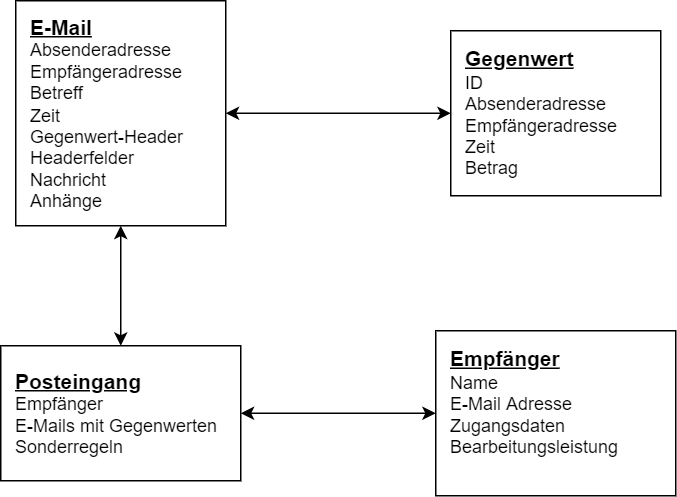
\includegraphics[width=0.75\textwidth]{Figures/Content Model.png}
	\caption{Content Model}
	\label{fig:content_model}
\end{figure}

\noindent Abbildung \ref{fig:content_model} zeigt das Modell. Als übergeordnetes Element kann der Posteingang verstanden werden, der pro Empfänger einmalig ist. Er enthält Informationen zum Empfänger, den E-Mails mit ihren Gegenwerten und Sonderregeln. Sonderregeln sind die in Kapitel \ref{Anforderungen_von_Empfaengern} thematisierten Abweichungen von der automatischen Triage. Der Empfänger besteht aus persönlichen Daten, sowie der Bearbeitungsleistung, die für die Einsicht relevant ist. Der Absender wurde im Content Model vernachlässigt, da er lediglich als E-Mail Adresse Teil des Systems ist; weitere Informationen über ihn sind nicht erforderlich. Die E-Mail enthält die für sie typischen Felder und den Gegenwert-Header, wie er in Kapitel \ref{Erkenntnisse_fuer_das_zu_entwickelnde_System} konzipiert wurde. Der Header enthält einen eindeutigen Identifikator, um den Gegenwert zuzuordnen. Der Gegenwert enthält grundlegende Informationen zur E-Mail, sowie den hinterlegten Betrag als Währung und Token.


%----------------------------------------------------------------------------------------

\section{Navigation Model}
\label{Navigation_Model}

Das Navigation Model beschreibt die einzelnen Bestandteile der Nutzeroberfläche und ihre Navigierbarkeit anhand von Pfeilen. Dabei unterscheidet es sich von Sequenzmodellen, wie einem UML-Ablaufdiagramm, ebenfalls dadurch, dass die Formulierung bewusst untechnisch ist und keinerlei Einfluss auf die Technologieentscheidung und Implementation hat. Da sich die Oberflächen für Absender und Empfänger grundlegend unterscheiden, werden zwei Modelle verwendet.

\begin{figure}[!ht]
	\centering
		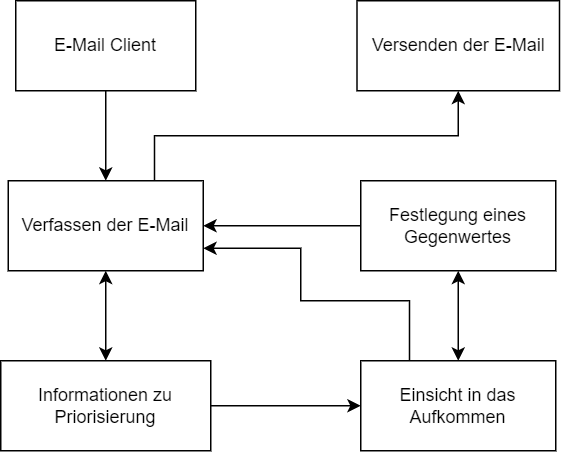
\includegraphics[width=0.75\textwidth]{Figures/Navigation Model Absender.png}
	\caption{Navigation Model des Absenders}
	\label{fig:navigation_model_absender}
\end{figure}

\noindent Das Navigation Model des Absenders in \ref{fig:navigation_model_absender} orientiert sich an den Use Cases 1 und 2. Es ist abhängig vom Mailclient, daher sind Abweichungen möglich. Grundlegend wird der Client gestartet und die Oberfläche zum Verfassen einer E-Mail aufgerufen. Der Nutzer erhält nach Eingabe des Empfängers die Information, dass Pay2Mail verwendet wird. Er kann diesen Hinweis ausblenden oder sich das Aufkommen des Empfängers ansehen. Hier hat er die Möglichkeit zurückzukehren oder einen Gegenwert zu hinterlegen, wobei er zurück zum Verfassen der E-Mail geleitet wird. Hier kann er, abhängig vom Client, die E-Mail vervollständigen und abschließend versenden.

\begin{figure}[!ht]
	\centering
		\includegraphics[width=0.75\textwidth]{Figures/Navigation Model Empfänger.png}
	\caption{Navigation Model des Empfängers}
	\label{fig:navigation_model_empfaenger}
\end{figure}

Das Navigation Model des Empfängers (siehe Abbildung \ref{fig:navigation_model_empfaenger}) ist nicht prozessorientiert, daher ist die Navigation stets bidirektional. Zu Beginn erscheint die Liste der E-Mails, wobei die Triage bereits durchgeführt wurde. Der Nutzer kann eine E-Mail in der Liste auswählen und die Bearbeitung, bzw. Beantwortung beginnen. Hier können Abweichungen an der Priorität gesetzt werden, die vom Posteingang gespeichert werden. Außerhalb der Bearbeitung von E-Mails kann der Nutzer Sonderregeln definieren, die automatisch Abweichungen von der Triage vornehmen. Darüber hinaus können Einstellungen an der Anwendung vorgenommen werden, wie die eigene Bearbeitungsleistung zu verändern. Jeder Schritt ermöglicht es zurück zur Liste der E-Mails zurückzukehren.

Dadurch, dass die technische Konzeption an diesem Punkt noch aussteht, ist die inhaltliche Konzeption als Grundlage, jedoch nicht als festes Regelwerk zu verstehen. Es ist möglich, dass sich die Navigation im System während der Implementation verändert. Abweichungen von der inhaltlichen Konzeption werden an entsprechender Stelle festgehalten und begründet.
%!TEX root = ../main.tex
% Chapter 8

\chapter{Technische Konzeption des Systems}
\label{Technische_Konzeption_des_Systems}

Dieses Kapitel beschäftigt sich mit der technischen Konzeption des Systems, wobei die Erkenntnisse der Markt- und Forschungsrecherche aus Kapitel \ref{Erkenntnisse_fuer_das_zu_entwickelnde_System} als Basis für die Architektur dienen. 

\section{Auswahl der Programmsprache und Pattern}
\label{Auswahl_der_Technologie_und_Designpattern}

Im Folgenden sollen die zu verwendenden Sprachen und Software Pattern definiert und beschrieben werden. Hierbei wird versucht möglichst wenige Sprachen zu nutzen, um die Entwicklungszeit zu minimieren. Die Auswahl eines Patterns hängt von der Sprache ab. So definieren manche Sprachen ein Pattern vor (diese werden auch \emph{opinionated languages} genannt), während andere die Entscheidung beim Entwickler belassen.

Die für die Entwicklung relevanten Funktionen können in drei Module unterteilt werden: Erweiterung des Absender-Clients, Empfänger-Client und Zahlungsmodul. Die Erweiterung des Absender-Clients beschreibt Plugins, die unterschiedliche E-Mail Clients erweitern. Da hierfür keine universelle Anwendung geschaffen werden kann, wird ein Web-Frontend implementiert, welches von verschiedenen Clients dargestellt werden kann. Innerhalb des Frontends wird das Headerfeld generiert, welches der Nutzer daraufhin in seinem Client hinterlegen kann. Der Empfänger-Client ist eine neu zu entwickelnde Anwendung, die sowohl ein Backend zur Speicherung der priorisierten E-Mails, als auch ein Frontend zur Darstellung jener benötigt. Das Zahlungsmodul ist ein Backend, welches die Zahlungen verwaltet und speichert. Es wird sowohl vom Absender-Frontend, als auch von der Anwendung des Empfängers kontaktiert. Darüber hinaus verwaltet es die Token, die jedem Nutzer zur Verfügung stehen.

\subsection{Node.js}
\label{Node.js}

% Framework und die darunter liegende Sprache erwähnen
% Features und Möglichkeiten der Sprache
% Pros für unseren Anwendungsfall
% Contras für unseren Anwendungsfall


\subsection{Ruby on Rails}
\label{Ruby_on_Rails}

% Framework und die darunter liegende Sprache erwähnen
% Features und Möglichkeiten der Sprache
% Pros für unseren Anwendungsfall
% Contras für unseren Anwendungsfall

\subsection{Laravel}
\label{ss}

% Framework und die darunter liegende Sprache erwähnen
% Features und Möglichkeiten der Sprache
% Pros für unseren Anwendungsfall
% Contras für unseren Anwendungsfall

\subsection{Django}
\label{ss}

% Framework und die darunter liegende Sprache erwähnen
% Features und Möglichkeiten der Sprache
% Pros für unseren Anwendungsfall
% Contras für unseren Anwendungsfall

\subsection{Spring Boot}
\label{ss}

% Framework und die darunter liegende Sprache erwähnen
% Features und Möglichkeiten der Sprache
% Pros für unseren Anwendungsfall
% Contras für unseren Anwendungsfall

\section{Festlegung einer Systemarchitektur}
\label{Festlegung_einer_Systemarchitektur}

\subsection{Datenmodell}
\label{Datenmodell}

\subsection{Komponentendiagramm}
\label{Komponentendiagramm}
%!TEX root = ../main.tex
% Chapter 9

\chapter{Implementation eines Prototyps zum Bezahl- und Tokensystem}
\label{Implementation_eines_Prototyps_zum Bezahl-_und_Tokensystem}

Nach der Konzeption des Systems wird im Folgenden ein Prototyp implementiert, welcher das Bezahl- und Tokensystem so abbilden soll, dass es in einer Nutzerbefragung verwendet werden kann.  Der Quellcode des Prototyps ist unter \url{https://github.com/astrutz/masterthesis/tree/prototype} einsehbar. Der Branch \texttt{prototype} repräsentiert dabei den Code, der im Rahmen dieses Kapitel entsteht.
 Wo möglich wird die spätere Funktionsweise des Systems mit Beispieldaten simuliert. Der entwickelte Prototyp kann unter \url{https://proto.pay2mail.org/send} getestet werden. 
 
Durch den prototypischen Fokus kann ein Großteil der in Abbildung \ref{fig:Komponentenmodell} skizzierten Komponenten ausgelassen und in Kapitel \ref{Implementation_des_Systems} implementiert werden. Einzig relevant ist das Absender-Frontend, das zumindest in seiner Funktionsweise vollständig sein sollte. Auch das Design des User Interface (UI) kann außer Acht gelassen werden, da sich die Befragung lediglich auf die Auswahl des Bezahlsystems fokussiert. Zusätzlich zum Frontend wird das Backend so vorbereitet, dass die Ressourcen für den Absender Beispieldaten zurückgeben, die noch nicht in der Datenbank abgelegt werden. 

\section{Projekt Setup und Einrichtung einer CI/CD Pipeline}
\label{Projekt_Setup_und_Einrichtung_einer_CI/CD Pipeline}

Zur Erstellung eines neuen Rails-Projektes bietet Ruby on Rails den Befehl \texttt{rails new pay2mail}, wobei pay2mail der Name des Projektes ist. Daraufhin wird eine Ordnerstruktur erstellt, die von Rails vorgegeben ist. Die Ordnerstruktur ist in Anhang xyz dargestellt. Für den Prototypen ist insbesondere der Ordner \texttt{app/} interessant, da er sowohl die Controller, als auch Views und Assets, wie css-Dateien enthält. Startet man den Server mit dem Befehl \texttt{rails server}, ist er im Standard unter Port 3000 verfügbar.

Bevor die eigentliche Entwicklung des Prototypen beginnt, wird eine CI/CD Pipeline eingerichtet. Sie dient dazu mit jedem \texttt{git push} auf den master-Branch verschiedene Routinen zu durchlaufen, die die Lauffähigkeit und Qualität des Codes prüfen. So wird auch die Stabilität der Anwendung sicher gestellt. Da das Projekt bei GitHub versioniert wird, wird GitHub Actions verwendet. GitHub Actions ist eine CI/CD-Umgebung, die direkt in GitHub integriert ist \citep{GitHub2022}. Pipelines, hier auch Workflows genannt, können als .yml-Datei formuliert werden. Der vollständige Workflow für Pay2Mail ist in Anhang \ref{lst:pipeline} zu sehen.

\begin{listing}[!ht]
\inputminted[firstline=8, lastline=32, linenos]{yaml}{Listings/rubyonrails.yml}

\caption
    [Auszug: CI Pipeline mit Testing-Job (\texttt{rubyonrails.yml})]
    {Auszug: CI Pipeline mit Testing-Job (\texttt{.github/rubyonrails.yml})}

\label{lst:pipeline-testing}
\end{listing}

Zu Beginn wird definiert, dass die Pipeline bei jedem Push auf Master, sowie bei jedem Pull Request, der in Master gemergt werden soll, läuft. Daraufhin werden zwei Jobs definiert, die zwei voneinander unabhängige Abläufe beschreiben und parallel laufen. Der erste Job \texttt{test} läuft auf einer Ubuntu VM und führt mit einer eigens dafür aufgesetzten Datenbank Unittests, Integrationtests und Systemtests aus. Dazu wird nach der Definition von Datenbank und Betriebssystem die aktuelle Codebasis geladen, die Abhängigkeiten von Ruby und Rails werden installiert und das Datenbankschema wird intialisiert. Nach diesen Vorbereitungen werden die Tests selbst mit \texttt{bin/rake} ausgeführt. Rake ist ein in Rails integrierter Test Runner, die alle im Ordner \texttt{test/} abgelegten Tests ausführt. Während der Implementation der Anwendung werden Unit Tests und Integration Tests geschrieben, die Kernfunktionalitäten des Systems abdecken sollen. Die Pipeline zum Ausführen der Tests ist in Sourcecode \ref{lst:pipeline-testing} zu sehen.

Da sie zur Sicherung der Codequalität dienen, jedoch keinen direkten Einfluss auf die Anwendung, sowie die Nutzung haben, werden die Tests in dieser Arbeit nicht weiter thematisiert. Die Tests können jedoch im Ordner \texttt{test/controllers/} eingesehen werden.

\begin{listing}[!ht]
\inputminted[firstline=34, lastline=48, linenos]{yaml}{Listings/rubyonrails.yml}

\caption
    [Auszug: CI Pipeline mit Linting-Job (\texttt{rubyonrails.yml})]
    {Auszug: CI Pipeline mit Linting-Job (\texttt{.github/rubyonrails.yml})}
    
\label{lst:pipeline-linting}
\end{listing}


Außerhalb der Tests wird ein weiterer Job namens \texttt{lint} ausgeführt. Dieser läuft ebenfalls auf Ubuntu und führt verschiedene Befehle aus, die die Qualität des Codes prüfen. Auch hier wird zu Beginn die Codebasis geladen und die nötigen Dependencies werden installiert. Daraufhin wird \texttt{bundle audit --update} ausgeführt. Dieses Plugin prüft die Abhängigkeiten im \texttt{Gemfile} auf Sicherheitslücken, potenziell gefährliche Quellen und führt automatisch Updates auf Patch-Ebene aus. Mit \texttt{brakeman -q -w2} wird der Quellcode selbst auf Sicherheitslücken geprüft. Das Flag \texttt{-q} sorgt dafür, dass Logs so begrenzt werden, dass nur Probleme, aber keine allgemeinen Informationen geloggt werden; das Flag \texttt{-w2} definiert, dass sowohl Warnungen mit mittlerer als auch mit hoher Priorität ausgegeben werden sollen. Zuletzt wird \texttt{rubocop --parallel} ausgeführt. Rubocop ist ein Linter, also ein Tool zur statischen Analyse und Formatierung des Sourcecodes \citep{Batsov2022}. Die Pipeline zum Linting ist in Sourcecode \ref{lst:pipeline-testing} zu sehen.

Die Pipeline selbst enthält keine Informationen zum Deployment. Stattdessen wird dazu \textit{App Platform} von \textit{DigitalOcean} verwendet. App Platform bietet die Möglichkeit Sourcecode direkt als Web Anwendungen zu deployen, dabei wird Autodeploy verwendet, mit welchem der Server selbst erkennt in welcher Sprache eine Anwendung geschrieben ist und notwendige Befehle zum Deployment selbstständig ausführt \citep{DigitalOcean2022}. Um den Sourcecode der App zu definieren, wird das Repository samt Branch ausgewählt. Daraufhin lädt App Platform den Sourcecode selbstständig bei jedem Push und deployt die Anwendung, die unter einer bereits definierten URL, in diesem Fall \url{https://plankton-app-whbh9.ondigitalocean.app}, erreichbar ist. Der Vorteil von App Platform ist die einfache Konfiguration, wodurch das Hosting zu Beginn der Entwicklung von prototypischen Anwendungen vernachlässigt werden kann.

Um eine aussagekräftigere und einprägsamere URL zu nutzen, die sich Nutzer und Tester merken können, wurde die Domain \url{pay2mail.org} erworben. Die Weiterleitung auf die App Platform Anwendung geschieht durch den DNS-Eintrag \texttt{pay2mail.org. CNAME plankton-app-whbh9.ondigitalocean.app.} Ferner wurde ein SSL-Zertifikat erworben, um die Sicherheit der Nutzerdaten, insbesondere im späteren Zahlungsprozess, sicherzustellen.

\section{Absender-relevantes Backend mit Beispieldaten}
\label{Absender-relevantes_Backend_mit_Beispieldaten}

Wie bereits zuvor erwähnt, wird das Backend des Absenders lediglich mit Beispieldaten simuliert. Um sowohl das Aufkommen, als auch die Möglichkeiten zur Priorisierung anzuzeigen, werden die Routen \texttt{/priority} und \texttt{/capacity} implementiert. Rails bietet die Möglichkeit mit dem Befehl \texttt{rails generate controller} gefolgt vom Namen einen Controller samt View und Tests anzulegen. Da die Rails Konvention Ressourcennamen im Plural vorschreibt, werden sie \texttt{capacities} und \texttt{priorities} genannt. Um das Absender-Backend vom Empfänger-Backend zu unterscheiden, erhalten die Routen das Prefix \texttt{/send}. 

Zusätzlich wird eine Route unter \texttt{/send/} im \texttt{overview\_controller.rb} implementiert, die als Startseite für Absender fungiert und im späteren Verlauf von E-Mail Clients abgerufen werden kann. Damit der Nutzer die E-Mail Adresse des Empfängers nicht erneut eingeben muss, wenn sie bereits im E-Mail Client hinterlegt ist, kann die Route mit dem Query-Parameter \texttt{recipient} aufgerufen werden. Durch DRY und Code Over Convention kann der Controller minimal gehalten werden, wie in Sourcecode \ref{lst:overview_controller} zu sehen.

\begin{listing}[!ht]
\inputminted[linenos]{ruby}{Listings/overview_controller.rb}

\caption
    [Controller für Absender-Frontpage (\texttt{overview\_controller.rb})]
    {Controller für Absender-Frontpage (\texttt{app/controllers/sender/overview\_controller.rb})}
    
\label{lst:overview_controller}
\end{listing}

\noindent Die Route \texttt{/capacity} zum Anzeigen des Aufkommens muss verpflichtend mit dem Query-Parameter \texttt{recipient} aufgerufen werden. In der späteren Anwendung werden die Bearbeitungsleistung, sowie die offenen Mails aus der Datenbank geladen. Für den Prototyp werden, wie in Sourcecode \ref{lst:capacities_controller} zu sehen, Standardwerte formuliert. So hat der Empfänger 107 E-Mails und eine Bearbeitungsleistung von 9 E-Mails pro Tag. Zusätzlich lassen sich auch diese Werte mit Query-Parametern festlegen. Dies ist notwendig, um Unit Tests formulieren zu können. Bei der Route \texttt{/priority} wird darauf verzichtet die Bearbeitungsleistung, sowie die offenen E-Mails im Backend zu definieren. Dazu müsste eine Liste von E-Mails mit spezifischen Zahlungen erzeugt werden, aus welcher die notwendigen Zahlungen für eine Priorisierung errechenbar wären. Diese Implementation würde bereits auf Model-Ebene notwendig sein und übertrifft den Rahmen des Prototyps. Stattdessen werden Testdaten im Frontend definiert.  

\begin{listing}[!ht]
\inputminted[linenos]{ruby}{Listings/capacities_controller.rb}

\caption
    [Controller für Empfänger-Aufkommen (\texttt{capacities\_controller.rb})]
    {Controller für Empfänger-Aufkommen (\texttt{app/controllers/sender/capacities\_controller.rb})}

\label{lst:capacities_controller}
\end{listing}

\section{Vorläufiges Absender-Frontend}
Für das Frontend wurden Views für die Absender-Übersicht, das Empfängeraufkommen und die Priorisierung implementiert. Screenshots der einzelnen Seiten sind in den Anhängen \ref{fig:screenshot_send/overview}, \ref{fig:screenshot_send/capacity} und \ref{fig:screenshot_send/priority} zu finden. Darüber hinaus steht der Prototyp unter \url{https://proto.pay2mail.org/send} zur Verfügung.

Das Frontend wird mit Bootstrap umgesetzt. Bootstrap ist eine Frontend-Library, die es Entwicklern ermöglicht vorgefertigte Komponenten zu verwenden, die nach einem Styleguide entwickelt wurden \citep{Twitter2022}. Bootstrap lässt sich mit verschiedenen Variablen individualisieren und bietet ein 12-spaltiges Gridlayout, welches responsive Anwendungen unterstützt. Da der Fokus des Prototyps, sowie der späteren Anwendung, auf der Funktionalität und Lösung des Problems der E-Mail Triage liegt, wird Bootstrap mit minimalen Anpassungen bezüglich Farbe und Abständen verwendet.

Das Frontend zur Startseite des Absenders besteht lediglich aus einem Eingabefeld für die Empfängeradresse, sowie zwei Buttons zur Weiterleitung auf \texttt{/capacity} oder \texttt{/priority}. Ist eine Empfängeradresse als Queryparameter enthalten, wird sie der View als Instanzvariable \texttt{@recipient} weitergegeben.

Das Aufkommen des Empfängers wird in drei umrahmten Elementen, von Bootstrap \textit{Card} genannt, umgesetzt. Die erste Card zeigt die Anzahl der offenen E-Mails des Empfängers, die zweite Card zeigt die Bearbeitungsleistung. Die dritte Card zeigt an, wann eine E-Mail ohne Priorisierung bearbeitet werden würde, wenn man sie jetzt abschickt. Das Markup dieser Card ist in Sourcecode \ref{lst:capacities/index} zu sehen. In Zeile 51 wird die Anzahl der E-Mails durch die Bearbeitungsleistung dividiert, um zu wissen wie viele Tage der Empfänger noch mit der Bearbeitung beschäftigt ist. Daraufhin wird ein Tag addiert für den Fall, dass die Bearbeitung für diesen Tag bereits abgeschlossen ist. Die Zahl wird aufgerundet und mit dem aktuellen Datum addiert, um ein potenzielles Bearbeitungsdatum zu erhalten. Der Aufruf \texttt{l} zu Beginn lokalisiert das Datum und zeigt es im Format TT.MM.JJJ an. Zusätzlich wird nach den Cards ein Informationstext über Priorisierung mit einem Link auf \texttt{/priority} angezeigt.

\begin{listing}[!ht]
\inputminted[firstline=43, lastline=55, linenos]{erb}{Listings/capacities_index.html.erb}

\caption
    [Auszug: View für Empfänger-Aufkommen (\texttt{capacities/index.html.erb})]
    {Auszug: View für Empfänger-Aufkommen (\texttt{app/views/sender/capacities/index.html.erb})}

\label{lst:capacities/index}
\end{listing}

\noindent Die View zu \texttt{/priority} erhält, wie bereits in Kapitel \ref{Absender-relevantes_Backend_mit_Beispieldaten} erwähnt, vom Controller keine Instanzvariablen oder sonstige Daten. Stattdessen sind die Beispieldaten direkt im Markup festgelegt. Die View zeigt einen Beschreibungstext zu Priorisierung an. Darunter wird eine Tabelle dargestellt, die dem Nutzer die Priorisierungsmöglichkeiten erläutert. Es werden verschiedene Termine aufgelistet, welche als vorläufiges Bearbeitungstermin dienen. Je kurzfristiger der Termin ist, desto höher ist der Preis, der für die Priorisierung zu zahlen ist. Außerdem wird als letzte Tabellenzeile der Termin angezeigt, an dem eine Bearbeitung ohne Priorisierung stattfinden würde.

Unterhalb der Tabelle kann der Nutzer einen Betrag (in Echtgeld) festlegen und die Zahlung bestätigen. Daraufhin wird er auf das Absender-Frontend weitergeleitet, welches eine Erfolgsmeldung mit einer UUID und Anweisungen zur Nutzung enthält. Diese UUID soll vom Empfänger, bzw. seinem E-Mail Client automatisiert, als E-Mail Header \texttt{X-Pay2Mail-Priority} gesetzt werden. 
%!TEX root = ../main.tex
% Chapter 10

\chapter{Nutzerbefragung zum Bezahl- und Tokensystem}
\label{Nutzerbefragung_zum Bezahl-_und_Tokensystem}
Das folgende Kapitel beschreibt die Konzeption und Durchführung einer nicht repräsentativen Umfrage zum Bezahl- und Tokensystem auf Basis des Prototyps aus Kapitel \ref{Implementation_eines_Prototyps_zum Bezahl-_und_Tokensystem}. Im Gegensatz zu einer detaillierten Systemevaluation soll die Befragung eine möglichst große Zahl an Antworten erzeugen, wie in Kapitel \ref{Vorgehensweise} erläutert. Die Ergebnisse der Befragung dienen als Grundlage für die Auswahl des Bezahl- und Tokensystems.

\section{Konzeption der Befragung}
Die Befragung wird zweiteilig gestaltet. Zu Beginn wird der Prototyp unter \\ \url{proto.pay2mail.org/send} vorgestellt. Die Teilnehmer haben die Möglichkeit eigenständig durch den Prototypen zu navigieren, ihnen wird dabei die Aufgabe gestellt eine dringende E-Mail zu versenden. Da sie das hohe Aufkommen des Empfängers sehen werden, sind sie aufgefordert die Zahlung zu tätigen. Dafür wird ein Betrag ausgewählt und abgesendet, ohne eine wirkliche Zahlung zu vollziehen. Den Teilnehmern wird bewusst keine Auswahl an Zahlungsmethoden oder Tokensystemen gegeben. So können sie sich mit dem System vertraut machen und die für sie durch Online-Shops o.ä. bekannteste Form des Gegenwertes nutzen.

Nachdem sie den Prototypen genutzt haben, werden den Teilnehmern vier Fragen gestellt. Zu Beginn wird gefragt, welches System zur Priorisierung der Teilnehmer bevorzugt: Zahlung mit Echtgeld, Zahlung mit vorher ausgehändigten Token oder Verbot von Zahlungen zur Priorisierung. Obwohl letztere Option das Problem der Priorisierung aus Kapitel \ref{Problemfeld_und_Folgen} nicht lösen würde, wurde sie trotzdem in die Befragung eingebunden, um eine mögliche Nutzerakzeptanz des späteren Systems erahnen zu können. Würde sich eine große Zahl an Teilnehmer gegen eine Zahlung im Generellen entscheiden, würde dies die Frage aufwerfen inwieweit Pay2Mail genutzt werden würde. Die restlichen Fragen beziehen sich auf Stamminformationen der Teilnehmer: Alter, Geschlecht und Jahresbruttoeinkommen. Diese Stamminformationen haben keinen direkten Bezug zum Bezahlsystem, geben aber die Möglichkeit Schlussfolgerungen zu ziehen und die Ergebnisse im Kontext zu betrachten. 

Während der Nutzung des Prototyps und der Befragung werden die Teilnehmer in Präsenz beaufsichtigt, um aufkommende Fragen zu klären. Daher wird die Befragung mündlich durchgeführt, die Ergebnisse werden notiert. So können sich die Teilnehmer auf den Prototypen und das Bezahlsystem fokussieren.

\noindent Die Teilnehmer werden über soziale Medien, Unternehmen und dem erweiterten Bekanntenkreis so zusammengesetzt, dass sie eine möglichst heterogene Menge hinsichtlich ihrer Stamminformationen ergeben. Außerdem wird bei der Auswahl der Teilnehmer auf einen souveränen und häufigen E-Mail Verkehr geachtet. So wird vermieden, dass Teilnehmer befragt werden, die mit E-Mails selten in Kontakt kommen und kein Interesse an der Thematik haben. Die Souveränität im Umgang mit E-Mails ist erforderlich, damit die Teilnehmer bereits mit der Problematik von Triage und Priorisierung vertraut sind und die Ineffizienz des E-Mail Standardheaders \textit{Priority} kennen.

\section{Ergebnisse der Befragung}
\label{Ergebnisse_der_Befragung}
Es wurden 39 Personen im Alter von 18 bis 62 und einem Jahresbruttoeinkommen von 900€ bis 105.000€ befragt. Davon haben 17 angegeben, dass sie männlich und 18 angegeben, dass sie weiblich sind. 4 Personen wollten keine Angabe machen. Die vollständigen Rohdaten der Befragung sind in Anhang \ref{tab:rohdaten} zu finden.

Die Mehrheit der Befragten (61,5\%) entschied sich dabei für ein Zahlungssystem mit Echtgeld, während sich 23,1\% für ein Tokensystem und 15,4\% gegen eine Zahlung im Allgemeinen aussprachen. Allerdings lassen sich große Unterschiede je nach Einkommen feststellen, wie in Abbildung \ref{fig:Auswahl_des_Zahlungssystems_der_Befragten_nach_Jahresbruttoeinkommen} zu sehen. So gibt es in der Gruppe der Jahresbruttoeinkommen kleiner als 20.000€ keine Mehrheit für ein System, stattdessen sind die Stimmen gleich verteilt. In der Gruppe der Einkommen zwischen 20.000€ und 40.000€ findet sich eine ähnliche Verteilung wie in der Gesamtzahl der Stimmen mit 66,7\% für Echtgeld, 25\% für Token und 8,3\% gegen ein Zahlungssystem. In der darauf folgenden Gruppe der Einkommen (40.000€ bis 60.000€) verändert sich die Verteilung stark zugunsten der Zahlung mit Echtgeld. Diese erreicht mit 81,8\% einen Höchstwert, während Zahlungen mit Token und die Ablehnung der Zahlung (jeweils 9,1\%) deutlich weniger Befragte überzeugen.

\begin{figure}[!ht]
\centering
\caption[Ergebnisse der Befragung nach Jahresbruttoeinkommen]{Ergebnisse der Befragung nach Jahresbruttoeinkommen}
\begin{tikzpicture}
    \begin{axis}[
        ybar,
        ymin=0,ymax=10,
        x label style={at={(axis description cs:0.5,-0.03)},anchor=north},
        y label style={at={(axis description cs:0.01,0.4)},anchor=west},
        ylabel= \textbf{Antworten},
        xlabel= \textbf{Jahresbruttoeinkommen},
        enlarge x limits  = 0.1,
        enlarge y limits  = 0.02,
        symbolic x coords={Unter 20.000€,20.000€ bis 40.000€,40.000€ bis 60.000€,Über 60.000€},
        xtick=data,
        width=0.99\textwidth,
        legend pos=north west
    ]
    \addplot coordinates
    {(Unter 20.000€, 4) (20.000€ bis 40.000€, 8) (40.000€ bis 60.000€, 9) (Über 60.000€, 3)};
    \addplot coordinates
    {(Unter 20.000€, 4) (20.000€ bis 40.000€, 3) (40.000€ bis 60.000€, 1) (Über 60.000€, 1)};
    \addplot coordinates
    {(Unter 20.000€, 4) (20.000€ bis 40.000€, 1) (40.000€ bis 60.000€, 1) (Über 60.000€, 0)};
    \legend{Echtgeld, Token, Keine Zahlung}
    \end{axis}
\end{tikzpicture}
\label{fig:Auswahl_des_Zahlungssystems_der_Befragten_nach_Jahresbruttoeinkommen}
\end{figure}

Diese drei Gruppen können miteinander verglichen werden, da sie in ähnlicher Häufigkeit in der Befragung vorkommen (jeweils 12, 12 und 11 Befragte). Die Gruppe der Einkommen größer als 60.000€ lässt sich hingegen nicht vergleichen, da hier lediglich vier Angaben vorliegen. Allerdings gibt es in dieser Gruppe nur eine Stimme gegen Echtgeld.

Aus den Daten lässt sich schlussfolgern, dass die Bereitschaft für eine Priorisierung zu zahlen, insbesondere mit Echtgeld, steigt je höher das eigene Einkommen ist. Das bedeutet allerdings auch, dass Personen mit einem niedrigeren Einkommen bei der Nutzung von Pay2Mail potenziell benachteiligt werden. Diese Problematik wird in Kapitel \ref{Schluss} näher behandelt. 

Hinsichtlich Geschlecht lassen sich keine weiteren Schlüsse ziehen. Die Ergebnisse von männlichen und weiblichen Befragten (64,7\% und 66,7\% für Echtgeld; 23,5\% und 22,2\% für Token; 11,8\% und 11,1\% gegen Zahlungen) ähneln den Gesamtergebnissen, siehe Abbildung \ref{fig:Ergebnisse_der_Befragung_nach_Geschlecht}. Die Anzahl der Befragten ohne Angabe des Geschlechts beläuft sich auf vier, was keine tragfähigen Aussagen zulässt. Auch bezogen auf das Alter der Befragten lassen sich keine weiteren Schlüsse folgern, siehe Abbildung \ref{fig:Ergebnisse_der_Befragung_nach_Alter}. In jeder Altersklasse, in Zehnjahresstufen unterteilt, überwiegt Echtgeld als bevorzugtes Zahlungssystem. Der niedrigste Zustimmungswert ist dabei 42,9\% in der Gruppe der 20- bis 30-Jährigen; der höchste Zustimmungswert ist 100\% in der Gruppe der über 60-Jährigen, wobei hier nur zwei Stimmen gezählt wurden. Die Ergebnisse für Echtgeld sind auch in den Gruppen der 30- bis 40-Jährigen (85,7\%) und 50- bis 60-Jährigen (87,5\%) sehr hoch.

\section{Auswahl eines Bezahl- und Tokensystems}
\label{Auswahl_eines_Bezahl-_und_Tokensystems}
Die Mehrheit der Befragten entschied sich in der Umfrage für ein Bezahlsystem mit Echtgeld. Die Entscheidung war über alle anhand von Geschlecht, Alter und Einkommen relevanten klassifizierten Gruppen eindeutig (siehe \ref{Ergebnisse_der_Befragung}). 

Die einzige Ausnahme ist die Gruppe der Jahresbruttoeinkommen unter 20.000€, welche keine Mehrheiten aufweist. In der Befragung gaben 12 der 39 Teilnehmer an, dass sie unter 20.000€ im Jahr netto verdienen, was etwa 31\% der Gesamtmenge der Befragten entspricht. Im Gegensatz dazu ergab eine Stichprobe \citep[S. 25 f.]{StatistischesBundesamt2018}, dass lediglich 17,8\% der Befragten ein Jahresbruttoeinkommen von unter 20.000€ haben. Das lässt darauf schließen, dass der Anteil in der durchgeführten Umfrage unverhältnismäßig groß war im Vergleich zur Stichprobe des statistischen Bundesamtes.

Unter diesem Gesichtspunkt ist es vertretbar Echtgeld als Zahlungsform von Pay2Mail zu nutzen. Allerdings sollte nach Einführung des Systems geprüft werden, inwiefern Personen mit geringerem Einkommen benachteiligt werden. Nach der Implementation und Evaluation des Systems wird die Frage der sozialen Gerechtigkeit bei der Priorisierung von E-Mails in Kapitel \ref{Reflektion_und_Bewertung} weiter thematisiert. 

\chapter{Implementation des Systems}
\label{Implementation_des_Systems}
Im Folgenden wird die Implementation des Systems erläutert, wobei zu Beginn Arbeitspakete definiert werden, die daraufhin bearbeitet werden. Die Dokumentation der Implementation wird, wo notwendig, mit Auszügen des Sourcecodes erweitert. Der vollständige Sourcecode ist unter \url{https://github.com/astrutz/masterthesis} zu finden, eine Instanz zum Testen liegt unter \url{https://pay2mail.org} vor.

\section{Umwandlung der Anforderungen in Arbeitspakete}
Um die in Kapitel \ref{Definition_von_Nutzeranforderungen} definierten Nutzeranforderungen zu strukturieren und die Entwicklung einzelner Features klar abzugrenzen, werden Arbeitspakete erstellt. Die Arbeitspakete werden so sortiert, dass die Anforderungen mit der höchsten Priorität zu Beginn implementiert werden. Das hat den Vorteil, dass bei fehlenden zeitlichen Ressourcen die wichtigsten Features bereits implementiert sind und Pay2Mail trotzdem nutzbar ist, wenn auch mit kleineren Einschränkungen. Tabelle \ref{tab:arbeitspakete} zeigt die Zuordnung der Anforderungen zu ihren jeweiligen Arbeitspaketen.

\begin{table}[!h]
\centering
\caption[Arbeitspakete der Implementation]{Zuordnung der Anforderungen zu Arbeitspaketen}
\begin{tabular}{|l|l|}
\rowcolor{red!25}
\hline
\textbf{Nutzeranforderung}               & \textbf{Arbeitspaket}            \\ \hline
Einsicht in das Aufkommen des Empfängers & Einsicht in das E-Mail Aufkommen \\ \hline
Priorisierbarkeit mit Gegenwert          & Priorisierung von E-Mails        \\ \hline
Technologisch unabhängige Nutzung        & -                                \\ \hline
Sicherheit der E-Mails und Zahlungen     & -                                \\ \hline
Keine Verlangsamung des E-Mail Prozesses & -                                \\ \hline
Automatische Triage                      & Automatische Triage              \\ \hline
Definition der Bearbeitungsleistung      & Einsicht in das E-Mail Aufkommen \\ \hline
Integrität der E-Mails und Zahlungen     & -                                \\ \hline
Abweichungen der automatischen Triage    & Automatische Triage              \\ \hline
Erreichbarkeit                           & -                                \\ \hline
Koexistenz zu bisherigen Kanälen         & -                                \\ \hline
Intuitive Nutzung                        & -                                \\ \hline
\end{tabular}
\label{tab:arbeitspakete}
\end{table}

\noindent Grundsätzlich werden obligatorische drei Arbeitspakete, sowie ein optionales Arbeitspaket, formuliert. Das erste Paket implementiert die Einsicht in das E-Mail Aufkommen. Hierfür wird das Frontend des Prototyps um Realdaten erweitert. Um Realdaten zu erhalten, werden die notwendige Datenstruktur und das Backend aufgesetzt, welches die E-Mails des MDA abruft. Daraufhin wird das Paket zur Priorisierung von E-Mails implementiert. Dabei wird die Datenstruktur um (simulierte) Zahlungen und die Priorität erweitert, auch hier wird das Frontend des Prototyps weiter verwendet. Die automatische Triage bildet das dritte Arbeitspaket ab, bei welcher eine Erweiterung der Datenbasis um Abweichungen der Triage notwendig wird. Außerdem wird ein Service implementiert, der die eigentliche Triage übernimmt. Das vierte Arbeitspaket ist die Anbindung realer Zahlungsanbieter. Dieser Schritt wurde bewusst ausgelagert, da er die Recherche nach APIs zur Abwicklung von Zahlungen und die Erweiterung der Architektur aus den Abbildungen \ref{fig:Datenmodell} und \ref{fig:Komponentenmodell} miteinbezieht. Dadurch bringt die Anbindung der Zahlungsanbieter eine größere Komplexität mit, die den zeitlichen Rahmen dieser Arbeit übersteigt. Das Arbeitspaket wurde jedoch trotzdem definiert als Ausblick, sowie als mögliches Zusatzfeature, falls die Implementation schneller abgeschlossen wird als vermutet. Andernfalls wird Pay2Mail so vorbereitet, dass die spätere Anbindung eines Zahlungsanbieters mit möglichst wenig Aufwand umsetzbar ist. 

In der Zuordnung in Tabelle \ref{tab:arbeitspakete} ist zu sehen, dass ein Großteil der Nutzeranforderungen nicht in Arbeitspakete überführt wird. Das hängt damit zusammen, dass sie bereits implizit durch die Architektur oder technische Grundvoraussetzungen umgesetzt werden. Die technologisch unabhängige Nutzung ist durch die Implementation als Webseite gegeben. Da die Einbindung mehrerer E-Mails Clients über den zeitlichen Rahmen dieser Arbeit hinausgeht, wird lediglich das Web-Frontend implementiert, welches die einzelnen Clients individuell integrieren können. Die Sicherheit der E-Mails bleibt Aufgabe der Clients, da der Versand weiterhin über sie stattfindet. Die Sicherheit der Zahlungen hingegen wird durch die Nutzung von HTTPS und verschlüsselten Datenbanken gewährleistet. Diese Features gehören zum Standard von Ruby on Rails und müssen daher nicht separat implementiert werden. Damit der E-Mail Prozess nicht verlangsamt wird, wird der Code in der CI/CD Pipeline auf verschiedene Fehlerquellen untersucht, die die Anwendung verlangsamen können, siehe dazu auch Kapitel \ref{Projekt_Setup_und_Einrichtung_einer_CI/CD Pipeline} und Sourcecode \ref{lst:pipeline}. Die Integrität der E-Mails und Zahlungen wird durch die Nutzung eines E-Mail Headers mit UUID sicher gestellt. Da die UUID in der Datenbank zusammen mit anderen Metadaten der E-Mail abgeglichen wird (siehe auch \ref{Datenmodell}), können Zahlungen nicht gefälscht oder wiederverwendet werden. Die Erreichbarkeit wird durch das Hosting bei DigitalOcean sichergestellt, welches bei Serverausfällen oder anderen Fehlern den Inhaber der Anwendung informiert. Die Koexistenz zu bisherigen Kanälen ist durch die Systemarchitektur impliziert, da E-Mails nicht ersetzt, sondern bei Bedarf nur erweitert werden. Die intuitive Nutzung der Anwendung ist eine Anforderungen, die sich nur unzureichend in konkrete Arbeitsschritte formulieren lässt. Stattdessen werden in der Implementation die Grundsätze der Dialoggestaltung nach ISO 9241-110 berücksichtigt, insbesondere \textit{Steuerbarkeit}, \textit{Erwartungskonformität}, \textit{Fehlertoleranz} und \textit{Selbstbeschreibungsfähigkeit} \citep{ISO9241-110}. Ob dies die intuitive Nutzung schlussendlich unterstützt, wird die Nutzerevaluation in Kapitel \ref{Nutzerevaluation_des_Systems} aufzeigen. 

%----------------------------------------------------

\section{Einsicht in das E-Mail Aufkommen}
\label{Einsicht_in_das_E-Mail_Aufkommen}

Das erste Arbeitspaket implementiert zwar die Einsicht des Absenders in das Aufkommen, darüber hinaus werden jedoch auch strukturelle Grundlagen geschaffen und das Datenbankschema umgesetzt. Zu Beginn werden die frontendseitigen Routen erweitert. Im Prototyp war es lediglich möglich mit \texttt{/send} auf die Übersicht des Absenderfrontends zu kommen, während die übergeordnete Route \texttt{/} einen 404-Fehler zurückgab. Zur Vorbereitung auf das später folgende Empfängerfrontend wurde eine Startseite implementiert, die die Möglichkeit bietet auf das Absenderfrontend oder das Empfängerfrontend zu wechseln. Ein entsprechender Screenshot ist in Anhang \ref{fig:screenshot_overview} zu sehen. Zur Trennung der beiden Frontendkomponenten werden zwei Namespaces verwendet, die in \texttt{routes.rb}, zu sehen in Sourcecode \ref{lst:routes}, deklariert werden. Die Namespaces fungieren als logische Klammern um das jeweilige Frontend und grenzen es innerhalb einer Route ab, sodass sich jede absenderbezogene Ressource unter \texttt{/send/*} und jede empfängerbezogene Ressource unter \texttt{/receive/*} befindet. Die Verbindung zwischen Namespace und späterer Route als \texttt{:sender} und \texttt{/send} wird mit dem Gem \texttt{route\_translator} realisiert, welches mehrsprachige Routen, sowie kanonische Benennung von Ressourcen ermöglicht \citep{LLuelles2022}. Der Namespace des Empfängers ist auskommentiert und wird im dritten Arbeitspaket implementiert.

\begin{listing}[!ht]
\inputminted[linenos]{ruby}{Listings/Pkg1/routes.rb}

\caption
    [Deklaration der HTTP-Routen]
    {Deklaration der HTTP-Routen (\texttt{config/routes.rb})}

\label{lst:routes}
\end{listing}

\noindent Zur Speicherung der Prioritäten und des Aufkommens wird das in Kapitel \ref{Datenmodell} konzipierte Datenmodell umgesetzt. Anpassungen der Datenbank werden in Rails stets in Migrationen umgesetzt. Eine Migration beschreibt welche Änderungen an der bestehenden Datenbank gemacht werden, wie Felder portiert werden und was mit Bestandsdaten passiert. Zur Erstellung einer Migration kann die Rails CLI genutzt werden mit dem Befehl \texttt{rails generate migration name\_der\_migration}. Daraufhin wird eine Migrationsdatei erstellt mit einer Funktion \texttt{change}, in welcher verschiedene Datenbankänderungen definiert werden, wie z.B. \texttt{create\_table}, zu sehen in Sourcecode \ref{lst:migration}. In diesem Beispiel wird die Tabelle für das Datenobjekt \texttt{Rule} erstellt mit den zwei Feldern als String. Zusätzlich wird die Assoziation zur \texttt{Inbox} aufgebaut, welche eine 1:n-Beziehung zu \texttt{Rule} hat. Da für solche Assoziationen bereits andere Tabellen vorhanden sein müssen, ist die Reihenfolge der Migrationen relevant. Es können mehrere Migrationen erstellt werden, bevor diese ausgeführt werden. Zur Ausführung wird der Befehl \texttt{rails db:migrate} genutzt. Erkennt Rails, dass es offene Migrationen gibt, kann der Server nicht gestartet werden, bis die Migrationen abgeschlossen sind. Das Datenbankschema wird in der Datei \texttt{schema.db} festgehalten und mit jeder Migration aktualisiert. Zudem werden Validierungen, Constraints und Assoziationen in den jeweiligen Models unter \texttt{app/models} festgehalten. Ebenfalls können Callbacks auf bestimmte Events genutzt werden.

\begin{listing}[!ht]
\inputminted[linenos]{ruby}{Listings/Pkg1/20220923155901_create_rules.rb}

\caption
    [Migration der Tabelle \texttt{Rules}]
    {Erstellung der Datenbanktabelle \texttt{Rules} als Migration (\texttt{db/migrate/20220923155901\_create\_rules.rb})}

\label{lst:migration}
\end{listing}

\noindent Um die Datenbank lauffähig und sicher zu gestalten, sind mehrere Anpassungen am Datenmodell notwendig. Die vorgesehene Beziehung zwischen \texttt{Value} und \texttt{Message} wurde aufgelöst. Zum Einen wird ein Gegenwert hinterlegt, bevor eine Nachricht versendet und somit in der Datenbank erstellt wurde, was eine intiale Beziehung nicht möglich macht. Außerdem verhindert eine Beziehung zwischen Nachricht und Gegenwert die direkte Überprüfung, ob ein Gegenwert zu einer Nachricht besteht und inwieweit die Metadaten der E-Mail übereinstimmen. Daher wird in der \texttt{Message} lediglich der Gegenwert-Header, also die UUID, gespeichert. Der \texttt{Value} enthält ebenfalls die UUID, sowie Metadaten zur E-Mail, wie anfänglich konzipiert. Allerdings ist die Speicherung aller E-Mail Header überflüssig, da bereits mit Versandzeitpunkt, Empfänger und Absender eine eindeutige Zuordnung möglich ist.
Im Datenmodell wurde die Verschlüsselung von Inhalten nicht betrachtet. Um jedoch die Anforderung \textit{Sicherheit der E-Mails und Zahlungen} einzuhalten, ist eine Verschlüsselung notwendig. Mit dem Gem \texttt{bcrypt} wird der Befehl \texttt{encrypts :feldname} hinzugefügt, welcher ausgewählte Datenbankfelder verschlüsselt.

\begin{listing}[!ht]
\inputminted[firstline=16, lastline=27,linenos]{ruby}{Listings/Pkg1/schema.rb}

\caption
    [Auszug: Definition von \texttt{Credentials} im Datenbankschema]
    {Auszug: Definition der Tabelle \texttt{Credentials} im Datenbankschema (\texttt{db/schema.rb})}

\label{lst:credentials}
\end{listing}

\noindent Außerhalb der Absicherung von Inhalten wurde ein wichtiger Bestandteil im Datenmodell ausgelassen. So sind zum Abrufen von E-Mails via IMAP entsprechende Zugangsdaten notwendig, die bisher jedoch nicht konzeptioniert wurden. Daher wird eine neue Tabelle \texttt{Credentials} erzeugt. Diese enthält den Servernamen als String, den Port als Integer, Informationen zu SSL und Authentifizierungstyp als String, sowie Nutzername und Passwort als String, welche jedoch verschlüsselt werden. Zudem wird eine 1:1-Beziehung zwischen \texttt{Recipient} und \texttt{Credential} definiert, wobei ein Credential nur so lange wie der Recipient existiert, sodass keine Anmeldedaten bei der Löschung eines Empfängers bestehen bleiben.

Um die Datenbank mit Nachrichten zu befüllen, wird folgend das Modul zum Abrufen der E-Mails implementiert. Da es noch nicht möglich ist aus dem Frontend Empfänger zu erstellen, werden zu Beginn Beispielnutzer mit realen IMAP-Daten erzeugt und der Datenbank hinzugefügt. Das Aufkommen dieser Nutzer lässt sich in der Testinstanz abrufen, die zugehörigen E-Mail Adressen lauten \\ \texttt{pay2mail-test01@freenet.de} und \texttt{pay2mail-test02@freenet.de}. Zur Umsetzung des Moduls wird \textit{ActiveJob} verwendet. ActiveJob ist ein Bestandteil von Ruby on Rails zur Ausführung von Routinen und Skripten (\textit{Jobs}) in einer Warteschlange. Außerdem ist es möglich Jobs zeitlich per \texttt{crontab} o.ä. zu planen und sie so regelmäßig auszuführen \citep{Hansson2022b}. Der Einstiegspunkt des Jobs ist die Funktion \texttt{perform}, die von Rails selbst oder Gems zur Verwaltung von Jobwarteschlangen angestoßen werden kann. Das Modul, benannt \texttt{EmailLoadJob}, iteriert durch eine Menge an Empfänger, meldet sich für jeden per IMAP beim MDA an, lädt alle ungelesenen E-Mails und speichert sie, falls nötig, in der Datenbank. Ein Auszug des Sourcecodes ist in \ref{lst:job} zu sehen, der vollständige Sourcecode ist in Anhang \ref{lst:job_full} abgebildet. Zur Nutzung des IMAP wird das Gem \textit{Mail} verwendet, welches Ruby-ähnliche Syntax bietet. Die zu iterierende Menge an Empfänger ist abhängig vom Kontext des Jobaufrufs. Daher wurde als reasonable default (siehe \ref{Ruby_on_Rails}) die Menge aller Empfänger gesetzt. So lässt sich der Job im Produktivbetrieb in einem Intervall ausführen und prüft die offenen E-Mails für alle Empfänger im Hintergrund. Außerdem lässt sich eine eigene Menge an Empfängern übergeben, so können beim Aufruf von \texttt{/capacity} die E-Mails eines Empfängers geprüft werden und das reale Aufkommen in Echtzeit dargestellt werden.

\begin{listing}[!ht]
\inputminted[firstline=4, lastline=11,linenos]{ruby}{Listings/Pkg1/email_load_job.rb}

\caption
    [Auszug: Job zum Laden der E-Mails]
    {Auszug: Job zum Laden der E-Mails beim MDN (\texttt{app/jobs/email\_load\_job.rb})}

\label{lst:job}
\end{listing}

\noindent Zur Darstellung des Aufkommens in Echtzeit muss der entsprechende Controller erweitert werden, siehe Sourcecode \ref{lst:capacities_controller_pkg1}. Anfangs wird in der Funktion \texttt{fetch\_recipient} anhand des übergebenen Queryparameters nach einem Empfänger in der Datenbank gesucht. Falls keiner gefunden wird, wird eine 404-Seite angezeigt mit dem Hinweis, dass der entsprechende Empfänger Pay2Mail nicht nutzt. Wird jedoch ein Empfänger gefunden, wird daraufhin der Job zum Laden der E-Mails mit der Empfängeradresse gestartet. Anhand des Empfängers wird der zugehörige Posteingang und die Anzahl der enthaltenen Nachrichten geladen. Da die Nachrichten nur so lange im Posteingang verweilen, bis sie bearbeitet wurden, kann diese Summe genutzt werden. Eine Nachricht gilt als bearbeitet, sobald sie vom Empfänger als gelesen markiert wurde. Diese Mechanik wird in Kapitel \ref{Automatische_Triage} genauer erläutert. Zusätzlich wird die Bearbeitungsleistung des Empfängers aus der Datenbank geladen. Zuletzt wird das voraussichtliche Antwortdatum berechnet, analog zum Vorgehen im Prototypen. Hierbei ist die Berechnung nun aus der View in den Controller ausgelagert worden, um die MVC-Architektur zu wahren. In der View zu \texttt{/capacities} werden die im Controller befüllten Instanzvariablen \texttt{@mails\_count}, \texttt{@editing\_performance} und \texttt{@target\_date} lediglich ausgegeben.

\begin{listing}[!ht]
\inputminted[linenos]{ruby}{Listings/Pkg1/capacities_controller.rb}

\caption
    [Erweiterter Controller für Empfänger-Aufkommen]
    {Erweiterter Controller für Empfänger-Aufkommen mit Realdaten (\texttt{app/controllers/sender/capacities\_controller.rb})}

\label{lst:capacities_controller_pkg1}
\end{listing}

%----------------------------------------------------

\section{Priorisierung von E-Mails}
\label{Priorisierung_von_E-Mails}
Das zweite Arbeitspaket verbindet das zuvor erstellte Datenbankschema mit Realdaten, sodass E-Mails priorisiert werden können. Damit Nutzer sehen können wie viel sie für die Priorisierung an einem bestimmten Tag zahlen müssen, wird die Tabelle auf der Seite \texttt{/send/priority} (vgl. Anhang \ref{fig:screenshot_send/priority}) so angepasst, dass sie das Aufkommen aus der Datenbank anzeigt. Da das Model \texttt{Message} lediglich die UUID, aber nicht den Gegenwert selbst enthält, muss vorher eine entsprechende Verknüpfung aufgebaut werden. Dazu iteriert die Funktion \texttt{with\_value} im Model \texttt{Message}, siehe Sourcecode \ref{lst:message1}, durch eine Menge an Nachrichten und sucht einen entsprechenden \texttt{Value}. Hierbei werden die UUID, die Adressen von Empfänger und Absender, sowie das Versanddatum der E-Mail geprüft. Das Versanddatum wird mit der Erstellungszeit des \texttt{Value}, dem automatisch generierten Feld \texttt{created\_at}, verglichen. Da die Zahlung und das Versenden der E-Mail nicht zeitgleich geschehen, wird eine Karenzzeit von 30 Minuten gegeben, nach welcher eine E-Mail versendet sein muss, um einem Gegenwert zugeordnet werden zu können. Dieses zeitliche Limit ergibt sich aus der Anforderung \textit{Sicherheit der Zahlungen}. Nach der Verknüpfung wird das Feld \texttt{value\_header} mit der Höhe des Gegenwertes überschrieben oder leer gelassen, falls kein Gegenwert-Header vorhanden ist.

\begin{listing}[!ht]
\inputminted[firstline=4, lastline=20,linenos]{ruby}{Listings/Pkg2/message.rb}

\caption
    [Auszug: Verknüpfung der Nachrichten mit ihren Gegenwerten]
    {Auszug: Verknüpfung der Nachrichten mit ihren Gegenwerten (\texttt{app/models/message.rb})}

\label{lst:message1}
\end{listing}

\noindent Um die Nachrichten nach ihren voraussichtlichen Bearbeitungstagen zu gruppieren, müssen sie zuerst sortiert werden. Dafür wird das neu befüllte Feld \texttt{value\_header} verwendet, das die Höhe der Zahlungen enthält. Die Sortierung erfolgt nach diesem Feld, E-Mails, die keinen Gegenwert enthalten, werden rückwärts nach ihrem Versanddatum sortiert. Das bedeutet, dass die Liste zuerst die E-Mails mit absteigendem Gegenwert und dann die E-Mails ohne Gegenwert mit aufsteigendem Versanddatum enthält. So ist sichergestellt, dass zuerst E-Mails mit Gegenwert und danach die ältesten E-Mails ohne Gegenwert bearbeitet werden. Daraufhin werden die E-Mails der jeweiligen Tage gruppiert. Dazu iteriert eine Schleife über die sortierte Liste und fügt jede Nachricht der Gruppe des aktuellen Tages \texttt{current\_group} hinzu. Sobald der Index der Schleife durch die Bearbeitungsleistung des Empfängers teilbar ist, wird die Gruppe der Gesamtmenge hinzugefügt und geleert. Die Teilbarkeit des Index zeigt an, dass eine Gruppe exakt die Größe hat, die vom Empfänger an einem Tag bearbeitet werden kann. Daher wird sie daraufhin der Gesamtmenge hinzugefügt. Diese Gruppierung wird für jede Nachricht wiederholt, wobei die letzte Gruppe unter Umständen weniger Nachrichten enthält, als der Empfänger an einem Tag bearbeitet. Die Gesamtmenge der Gruppierung ist ein Array, das wiederum für jeden Tag ein Array an Nachrichten enthält, das zu bearbeiten ist. Die erste Gruppe in der Gesamtmenge spiegelt die Nachrichten für \textit{Morgen} wieder, die zweite Gruppe spiegelt die Nachrichten für \textit{Übermorgen} wieder usw. Der Algorithmus zur Gruppierung ist in Sourcecode \ref{lst:message2} dargestellt.

\begin{listing}[!ht]
\inputminted[firstline=22, lastline=38,linenos]{ruby}{Listings/Pkg2/message.rb}

\caption
    [Auszug: Gruppierung der Nachrichten nach Gegenwerten]
    {Auszug: Gruppierung der Nachrichten nach Gegenwerten basierend auf der Bearbeitungsleistung des Empfängers (\texttt{app/models/message.rb})}

\label{lst:message2}
\end{listing}

\noindent Die gruppierten Nachrichten ermöglichen es nun die Tabelle der Priorisierung zu befüllen. Dazu wird in der View durch die gruppierten Nachrichten \texttt{@messages\_grouped} iteriert und für jede Gruppe eine neue Zeile in der Tabelle erzeugt, siehe Sourcecode \ref{lst:capacities/index_pkg2}. Dabei werden Gruppen übersprungen, deren Gegenwert identisch zum Gegenwert der folgenden Gruppe ist. Das ist notwendig, da eine neue E-Mail jeweils am Ende der Nachrichten mit dem gleichen Gegenwert einsortiert wird, da sie die Neueste ist. Sind beispielsweise für die nächsten drei Tage E-Mails mit einem Gegenwert von 5,00€ eingeplant, würde eine neue E-Mail mit dem selben Gegenwert erst in vier Tagen bearbeitet werden. In diesem Fall wird erst die letzte Tabellenzeile mit den E-Mails für 5,00€ angezeigt, da die neue E-Mail dort eingereiht wird. Als vorläufiges Bearbeitungsdatum werden jeweils zwei Tage addiert, da die erste Gruppe unter Umständen erst am nächsten Tag begonnen wird und sich die neue E-Mail dort einreihen müsste. Eine Ausnahme ist die letzte Gruppe, falls sie kleiner als die Bearbeitungsleistung ist. In dem Fall wird lediglich ein weiterer Tag addiert, da in dieser Gruppe noch ein Platz vorhanden ist. Als Preis wird der Gegenwert der letzten Nachricht pro Gruppe ausgewählt und um 1,00€ erhöht, sodass eine neue E-Mail vor der letzten E-Mail in der Gruppe eingereiht würde. Die Erhöhung des Preises um 1,00€ entspricht der Mindestdifferenz von Gegenwerten, die in dieser Iteration des Systems festgelegt wurde. Theoretisch könnte diese Differenz auch auf 0,01€ reduziert werden, allerdings würde dies dem Grundsatz des Gegenwertes widersprechen. Außerdem würde es dazu führen, dass Absender möglichst lange mit ihrer Priorisierung warten, um E-Mails aus einer Gruppe knapp zu überbieten.

\begin{listing}[!ht]
\inputminted[firstline=26, lastline=39, linenos]{erb}{Listings/Pkg2/priorities_index.html.erb}

\caption
    [Auszug: Generierung der Tabelle zur Priorisierung]
    {Auszug: Generierung der Tabelle zur Priorisierung von E-Mails (\texttt{app/views/sender/priorities/index.html.erb})}

\label{lst:capacities/index_pkg2}
\end{listing}

Unter der Tabelle wird ein Button angezeigt, der auf ein Formular zur Priorisierung der E-Mail verlinkt. Anhang \ref{fig:screenshot_send/priority_new} zeigt dieses Formular. Es ist an das Model \texttt{Value} geknüpft. Der Absender trägt seine E-Mail Adresse, die E-Mail Adresse des Empfängers, sowie den gewünschten Betrag ein und sendet das Formular ab. Im Controller wird daraufhin die Action \texttt{create} aufgerufen. Aus dem HTTP-Body des Requests werden die Formulardaten ausgelesen. Es wird eine neue Instanz von \texttt{Value} erzeugt und mit den Formulardaten befüllt. Nach Speicherung des Gegenwertes wird der Nutzer auf die Action \texttt{show} weitergeleitet. Diese öffnet ein entsprechendes Frontend und zeigt die UUID des \texttt{Value} zusammen mit dem voraussichtlichen Antwortdatum des Empfängers an, zu sehen in Abbildung \ref{fig:screenshot_send/priority_show}.

\begin{listing}[!ht]
\inputminted[firstline=14, lastline=23,linenos]{ruby}{Listings/Pkg2/priorities_controller.rb}

\caption
    [Auszug: Erstellung eines neuen Gegenwertes]
    {Auszug: Erstellung eines neuen Gegenwertes und Darstellung der generierten UUID (\texttt{app/controllers/priorities\_controller.rb})}

\label{lst:priorities_controller}
\end{listing}

\noindent Die Berechnung des voraussichtlichen Antwortdatums ist im Model \texttt{Value} umgesetzt. Hierzu werden alle Nachrichten des Empfängers aus der Datenbank geladen und wie zuvor beschrieben gruppiert. Daraufhin wird durch die Gruppierungen iteriert und für jede Iteration ein Tag zum Heutigen addiert und in \texttt{days\_to\_wait}. Dies wird wiederholt bis eine Gruppierung gefunden wird, welche einen kleineren Gegenwert als den eben erstellten Gegenwert enthält. Das daraus entstehende Datum wird als voraussichtliches Antwortdatum des Empfängers dargestellt. Der entsprechende Sourcecode ist in Anhang \ref{lst:value} zu finden.

%----------------------------------------------------

\section{Automatische Triage}
\label{Automatische_Triage}

Das Arbeitspaket der automatischen Triage ist das umfangreichste Paket, da verschiedene Aspekte und Funktionen kombiniert werden. Zu Beginn wird ein Mechanismus implementiert, der Login, Logout und Registrierung ermöglicht. Die Registrierung ist mit Interaktionen mit der Datenbank verbunden, da hier neue Instanzen von \texttt{Recipient} und \texttt{Credential} erzeugt werden. Außerdem wird die Empfängeransicht umgesetzt, welche nach erfolgreichem Login oder erfolgreicher Registrierung sichtbar ist und die E-Mails in einer priorisierten Liste anzeigt. Zusätzlich ist eine Detailansicht der E-Mails notwendig, die den eigentlichen Nachrichteninhalt anzeigt und die Möglichkeit bietet eine E-Mail zu \textit{erledigen}. Mit der Erledigung muss sowohl eine entsprechende Meldung an den MDA, als auch an die Datenbank erfolgen. Mit diesen Informationen können die Bearbeitungsleistung geprüft und präzise Fälligkeitsdaten für E-Mails vorhergesagt werden. Als zusätzliche Anforderung wird abschließend die Ausnahmefunktion implementiert, die es ermöglicht Regeln zu definieren, nach welchen E-Mails die Priorisierung umgehen können.

Zur Registrierung wird ein neuer Controller \texttt{recipients} angelegt, der die entsprechenden Ressourcen bereitstellt. Analog zur Priorisierung rendert die Action \texttt{recipients\#new} die Oberfläche zur Registrierung, die nach Absenden des Formulars in der Action \texttt{create} per POST-Request angestoßen wird. Die Action \texttt{new} erhält dabei den Pfad \texttt{/signup}, der für den Nutzer verständlicher ist und keine Hinweise auf das darunterliegende Datenbankmodell gibt. Die Action \texttt{create} erstellt eine neue \texttt{Inbox} und befüllt daraufhin einen neuen \texttt{Recipient} und einen neues \texttt{Credential} mit den Daten des HTTP-Body, gefolgt von der Speicherung. Schlägt das Speichern, beispielsweise aufgrund von nicht erfüllten Validierungen, fehl, wird das UI zur Registrierung erneut mit einer entsprechenden Fehlermeldung zurückgegeben. Andernfalls wird das Login des Nutzers übernommen (für weitere Informationen s.u.) und eine Weiterleitung auf den Posteingang vorgenommen. Sourcecode \ref{lst:recipients_controller} zeigt die Registrierung im Backend, wobei das Auslesen des HTTP-Body in \texttt{fill\_credentials} und \texttt{fill\_recipient} ausgelagert wurde.

\begin{listing}[!ht]
\inputminted[firstline=9, lastline=23, linenos]{ruby}{Listings/Pkg3/recipients_controller.rb}

\caption
    [Auszug: Registrierung eines neuen Empfängers]
    {Auszug: Registrierung eines neuen Empfängers im Backend (\texttt{app/controllers/receive/recipients\_controller.rb})}

\label{lst:recipients_controller}
\end{listing}

\noindent Zu Login und Logout wurde der Controller \texttt{sessions\_controller} angelegt, der keine korrespondierende Datenbankentität besitzt. Dies hängt damit zusammen, dass Anmeldungen nicht serverseitig persistiert werden, um die Datensicherheit der Empfänger zu wahren. Stattdessen wird der Status des Logins in der Session der Nutzers unter dem Schlüssel \texttt{recipient\_id} hinterlegt. Mit den Actions \texttt{new} und \texttt{create} wird das Frontend, sowie der Endpunkt zum Login bereitgestellt. Dabei werden die Anmeldedaten aus dem HTTP-Body abgeglichen, abhängig vom Ergebnis wird der Nutzer entweder auf den Posteingang oder die Login-Seite mit einer Fehlermeldung weitergeleitet. Diese Helfer-Methode ist im \texttt{application\_controller} abgelegt und daher global nutzbar. So binden sämtliche Controller im Empfängerscope \texttt{receive} lediglich die Funktion \texttt{authorize} als \texttt{before\_action}, also als ersten Aufruf nach dem Request, ein. Die Funktion sucht einen passenden \texttt{Recipient} für die Session und gibt entweder diesen zurück oder leitet auf die Login-Seite weiter, falls der Nutzer nicht eingeloggt ist. Analog dazu wird beim Logout der Schlüssel in der Session wieder geleert, gefolgt von einer Weiterleitung auf die Startseite. Login, Registrierung und Logout können über entsprechende Links im Header des UIs erreicht werden, welcher die Farbe ändert je nach dem, ob ein Nutzer angemeldet ist oder nicht. Die Farbänderung unterstützt den Nutzer dabei zwischen Absenderfrontend und Empfängerfrontend zu unterscheiden. Screenshots dazu finden sich in den Anhängen \ref{fig:screenshot_header1} und \ref{fig:screenshot_header2}. Der Login-Mechanismus ist in Sourcecode \ref{lst:application_controller} zu sehen. Es ist zu erwähnen, dass dieser Mechanismus nicht produktionsreif ist, da es zur Kompromittierung eines Empfängers ausreicht seine ID zu kennen, die im Klartext im Browser auszulesen ist. Um dies zu beheben müsste die ID nochmals verschlüsselt werden. Aufgrund des zeitlichen Rahmens des Projektes wird der Mechanismus nicht erweitert und der Domain \url{https://pay2mail.org} wird stattdessen eine Authentifizierung mit Basic Auth vorgeschaltet.

\begin{listing}[!ht]
\inputminted[linenos]{ruby}{Listings/Pkg3/application_controller.rb}

\caption
    [Auszug: Funktion zum Login von Empfängern]
    {Auszug: Globale Funktion zum Login von registrierten Empfängern (\texttt{app/controllers/application\_controller.rb})}

\label{lst:application_controller}
\end{listing}

\noindent Nach erfolgreicher Authentifizierung wird der Posteingang des Nutzers unter der Startseite für das Empfängerfrontend \texttt{/receive} angezeigt. Vor Anzeige des Frontends werden die ungelesenen E-Mails per \texttt{EmailLoadJob} geladen, wie in Kapitel \ref{Einsicht_in_das_E-Mail_Aufkommen} erläutert. Die \texttt{Inbox} und Liste von Nachrichten (\texttt{Message}) werden anhand der \texttt{recipient\_id} aus der Datenbank geladen. Die Liste der Nachrichten ist im Standard nach Erstelldatum in der Datenbank sortiert. Zur Sortierung nach Gegenwert wird die Liste mit den Gegenwerten in \texttt{with\_value} angereichert, wie in Kapitel \ref{Priorisierung_von_E-Mails} bereits erläutert. Die Funktion wird so erweitert, dass sie einen im Standard auf \texttt{false} gesetzten Parameter \texttt{sorted} annimmt, der bestimmt, ob die angereicherte Liste sortiert wird. Im Falle einer Sortierung wird die Funktion \texttt{sort\_by\_value} aufgerufen, die aus der Funktion \texttt{group\_by\_amount} extrahiert wurde. Im Frontend wurde die \texttt{Table}-Komponente von Bootstrap verwendet, die abwechselnd gefärbte Streifen und eine Änderung der Farbe bei Hover mit sich bringt. Ergänzend zu Betreff und Absender zeigt die Tabelle den gesetzten Gegenwert und das Versanddatum der Nachricht an. Abbildung \ref{fig:screenshot_inbox} zeigt einen Screenshot des Posteingangs.

\begin{figure}[!ht]
	\centering
		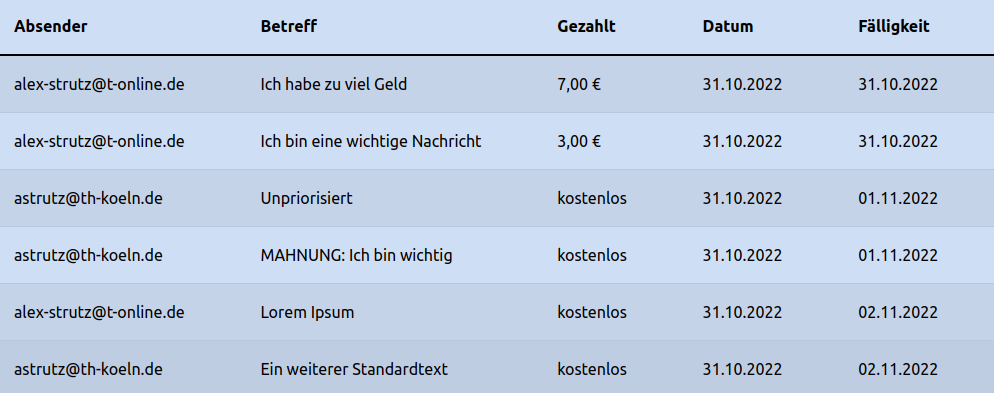
\includegraphics[width=1\textwidth]{Figures/inbox.png}
	\caption{Screenshot: Posteingang eines Empfängers, nach Priorität sortiert}
	\label{fig:screenshot_inbox}
\end{figure}

\noindent Mit Klick auf eine Tabellenzeile wird die entsprechende Nachricht in der Detailansicht \texttt{/receive/messages/:id} angezeigt. Anhand der ID wird die \texttt{Message} aus der Datenbank geladen und an das Frontend übergeben. Dieses zeigt die Nachricht, vergleichbar mit gängigen E-Mail Clients, in zweiteiliger Struktur aus Metadaten (E-Mail Header) und Inhalt (E-Mail Body) an. Anhang \ref{fig:screenshot_message} zeigt einen entsprechenden Screenshot. Zusätzlich wird ein \textit{Erledigt}-Button angezeigt, mit welchem ein Empfänger eine E-Mail als bearbeitet kennzeichnen kann. Dies ist jedoch nur bei E-Mails möglich, die am höchsten priorisiert sind. Bei Klick auf den Button wird die Action \texttt{messages\#destroy} aufgerufen. Die \texttt{Message} wird anhand des Query-Parameters ID geladen. Falls der Parameter \texttt{fetch} nicht gesetzt ist, es sich also nicht um einen Test handelt (vgl. \ref{Einsicht_in_das_E-Mail_Aufkommen}), wird der \texttt{EmailLoadJob} aufgerufen und die Nachricht mit \texttt{read\_message} gelesen. Dazu wird eine IMAP \texttt{SEARCH} ausgeführt, die die gefundene Nachricht als gelesen markiert. 

\begin{listing}[!ht]
\inputminted[firstline=8, lastline=17, linenos]{ruby}{Listings/Pkg3/messages_controller.rb}

\caption
    [Auszug: Erledigung einer Nachricht]
    {Auszug: Erledigung einer Nachricht durch Setzen eines Bearbeitungszeitpunktes (\texttt{app/controllers/receive/messages\_controller.rb})}

\label{lst:messages_controller}
\end{listing}

\noindent Darüber hinaus muss das System die Anzahl der erledigten Mails des \texttt{Recipient} je Tag vorhalten, um Aussagen über die noch zu erledigenden E-Mails tätigen zu können. Hierzu wird das Datenbankmodell der \texttt{Message} so erweitert, dass es einen Timestamp \texttt{processed\_at} enthält. Mit diesem Feld kann festgehalten werden ob und wann welche Nachricht erledigt wurde. Zusätzlich werden die Scopes \texttt{processed} und \texttt{unprocessed} implementiert. Scopes sind im Kontext von Ruby on Rails Datenbankselektionen, die auf Model-Ebene implementiert und daraufhin global mit \texttt{Model.scope} genutzt werden können \citep{Hansson2022c}. Im Falle der zuvor erwähnten Scopes führt \texttt{processed} die Query \texttt{where.not(processed\_at: nil)} und \texttt{unprocessed} die Query \texttt{where(processed\_at: nil)} aus. So können die bisherigen Views einfach angepasst werden, um nur unbearbeitete Nachrichten anzuzeigen. Die an einem Tag bearbeiteten E-Mails können im Scope \texttt{processed} mit einer Filterung nach dem Tag geladen werden. Sourcecode \ref{lst:messages_controller} zeigt die backendseitige Erledigung einer \texttt{Message}.

Mit dem implementierten Bearbeitungsdatum ist es nun möglich E-Mails für den Empfänger mit einem Fälligkeitsdatum zu versehen. Dazu wird beim Laden der Action \texttt{show} der \texttt{Inbox} die Funktion \texttt{calculate\_due\_dates} aufgerufen, siehe Sourcecode \ref{lst:inboxes_controller}. Diese Funktion erzeugt ein Array, welches die verschiedenen Fälligkeitsdaten enthält. Dazu wird eine Schleife durchlaufen. Für jede unbearbeitete Nachricht, nach Priorität sortiert, wird geprüft, ob ihr Index durch die Bearbeitungsleistung teilbar ist. Dabei werden die am heutigen Tag bearbeiteten E-Mails miteinbezogen. Ist der Rest der Division gleich 0, wird ein Tag zum Fälligkeitsdatum addiert. So entsteht ein Array an \texttt{DateTime}-Instanzen, das die gleiche Anzahl an Elementen wie die Liste an Nachrichten enthält. Das Array wird als Instanzvariable \texttt{@due\_dates} an die View übergeben, welche sie entsprechend in der Posteingangstabelle darstellt. 

\begin{listing}[!ht]
\inputminted[firstline=12, lastline=23, linenos]{ruby}{Listings/Pkg3/inboxes_controller.rb}

\caption
    [Auszug: Berechnung der Fälligkeitstermine]
    {Auszug: Berechnung der Fälligkeitstermine für Empfänger (\texttt{app/controllers/receive/inboxes\_controller.rb})}

\label{lst:inboxes_controller}
\end{listing}

\newpage

\noindent Zusätzlich zur Triage im Posteingang soll dem Empfänger die Möglichkeit gegeben werden Regeln zu definieren, nach welchen E-Mails die Triage überspringen und direkt bearbeitet werden können. Hierzu wird das Empfängerfrontend so erweitert, dass eine zweite Tabelle verfügbar ist, welche E-Mails enthält, auf welche die Regeln zutreffen. Diese E-Mails werden im Folgenden \textit{Ausnahmenachrichten} genannt. Die beiden Tabellen werden mit der \texttt{Tab}-Komponente von Bootstrap getrennt, sodass nur eine sichtbar ist und der Nutzer zwischen ihnen wechseln kann, siehe Anhang \ref{fig:screenshot_inbox2}. Der Posteingang listet weiterhin Ausnahmenachrichten auf, sodass der Empfänger sie regulär nach ihrer Fälligkeit bearbeiten kann, falls sie sich nach Sichtung als weniger relevant darstellen. Um zu ermitteln welche Nachrichten als Ausnahmenachrichten gelten, wird dem \texttt{Message}-Model ein weiterer Scope namens \texttt{matches\_rules} hinzugefügt, wie in Sourcecode \ref{lst:message3} zu sehen. Im Scope wird durch die Regeln des Posteingangs iteriert und für jede Regel eine Datenbankquery erzeugt, die nach Elementen sucht, die für das Feld definiert von \texttt{field\_to\_search} den Wert \texttt{field\_matcher} enthalten. Mögliche Werte für \texttt{field\_to\_search} sind \texttt{subject}, \texttt{sender\_address} oder \texttt{content}, die jeweils den Betreff, den Absender oder den Inhalt der E-Mail durchsuchen. Das Ergebnis der einzelnen Queries wird konkateniert und als Array, sortiert nach dem Versanddatum, zurückgegeben. Die Sortierung erfolgt bewusst nur nach dem Versanddatum und nicht nach dem Gegenwert, da dieser bei Ausnahmenachrichten nicht mehr relevant ist.

\begin{listing}[!ht]
\inputminted[firstline=6, lastline=15, linenos]{ruby}{Listings/Pkg3/message.rb}

\caption
    [Auszug: Scope zur Ermittlung der Ausnahmenachrichten]
    {Auszug: Scope zur Ermittlung der Ausnahmenachrichten für Empfänger (\texttt{app/models/message.rb})}

\label{lst:message3}
\end{listing}

\noindent Als letztes Feature wird das Anzeigen, Erstellen, Bearbeiten und Löschen (CRUD) von Regeln, sowie die Anpassung der Bearbeitungsleistung durch den Empfänger implementiert. Für Letztere werden dem \texttt{recipients\_controller} die Actions \texttt{edit} und \texttt{update} hinzugefügt. Dabei gibt \texttt{edit} ein Frontend zur Bearbeitung der Regeln, siehe Anhang \ref{fig:screenshot_recipients}, zurück. Bei Klick auf den Button wird die Action \texttt{update} aufgerufen, die den neuen Wert als \texttt{editing\_performance\_per\_day} speichert. Für die Regeln wurden entsprechende Views und Actions definiert, die dem bereits bekannten Schema folgen, benannt \texttt{new} und \texttt{create} zur Erstellung, \texttt{edit} und \texttt{update} zur Bearbeitung und \texttt{destroy} zum Löschen. Screenshots dieser Oberflächen finden sich in den Anhängen \ref{fig:screenshot_rules1} bis \ref{fig:screenshot_rules3}. Die Routenstruktur der finalen Anwendung ist in Anhang \ref{Routenstruktur_der_Anwendung} hierarchisch dargestellt.

%----------------------------------------------------------------------------------------
%	THESIS CONTENT - APPENDICES
%----------------------------------------------------------------------------------------

\appendix % Cue to tell LaTeX that the following "chapters" are Appendices

% Include the appendices of the thesis as separate files from the Appendices folder
% Uncomment the lines as you write the Appendices

% Appendix A

\chapter{Tabellen, Diagramme und Befragungsergebnisse}
\label{Tabellen_Modelle_Diagramme}

\section{Stakeholderanalyse}

\begin{table}[H]
	\centering
	\caption[Stakeholderanalyse]{Stakeholder für E-Mails in Unternehmen}
		\vspace{1.0em}	
    \begin{tabular}{|l|l|l|l|}
    \rowcolor{red!25}
    \hline
    \textbf{Bezeichnung}                   & \textbf{Beziehung} & \textbf{Objektbereich}                                             & \textbf{Prio} \\ \hline
    Absender              & Anrecht            & Unlimitierter Versand von E-Mails                                  & 1                  \\ \cline{2-4} 
                                           & Interesse          & Beantwortung von E-Mails                                           & 1                  \\ \cline{2-4} 
                                           & Interesse          & Voraussichtliche Antwortzeit                                       & 1                  \\ \hline
    Empfänger             & Anrecht            & Erreichbarkeit                                                     & 1                  \\ \cline{2-4} 
                                           & Anrecht            & Eigene Zeiteinteilung bei Triage                                   & 2                  \\ \cline{2-4} 
                                           & Interesse          & Strukturierte E-Mails                                              & 2                  \\ \cline{2-4} 
                                           & Interesse          & Benachrichtigung bei neuen E-Mails                                   & 1                  \\ \cline{2-4} 
                                           & Interesse          & Einfach erkennbare Priorität von E-Mails                           & 2                  \\ \hline
    Management            & Anspruch           & Produktivität von Mitarbeitern trotz E-Mails                       & 2                  \\ \cline{2-4} 
                                           & Anspruch           & Erreichbarkeit der Mitarbeiter                                     & 1                  \\ \hline
    ISP                                    & Anteil             & Anteil an externer Infrastruktur von E-Mails         & 2                  \\ \hline
    Administratoren & Anteil             & Interne Infrastruktur                                              & 1                  \\ \cline{2-4} 
                                           & Anteil             & Schutzmaßnahmen vor Spam und Angriffen via E-Mail                  & 2                  \\ \hline
    Betriebsräte                           & Interesse          & Interesse an sozialen Auswirkungen auf Empfänger & 3                  \\ \hline
    \end{tabular}
	\label{tab:stakeholderanalyse}
\end{table}
% ------------------------------------------------------


\section{Ergebnisse der Befragung zu Bezahl- und Tokensystemen}

\begin{table}[H]
\centering
	\caption[Rohdaten der Befragung]{Rohdaten der Befragung zu Bezahl- und Tokensystemen}
\begin{tabular}{lllll}
\rowcolor{red!25}
\hline
\multicolumn{1}{|l|}{\textbf{Nr.}} & \multicolumn{1}{l|}{\textbf{Geschlecht}} & \multicolumn{1}{l|}{\textbf{Alter}} & \multicolumn{1}{l|}{\textbf{Jahresbruttoeinkommen}} & \multicolumn{1}{l|}{\textbf{Auswahl}} \\ \hline
1                                  & w                                        & 61                                  & 21.402,36 €                             & Echtgeld                              \\
2                                  & m                                        & 53                                  & 51.985,88 €                             & Echtgeld                              \\
3                                  & m                                        & 44                                  & 49.219,10 €                             & Keine Zahlung                         \\
4                                  & m                                        & 32                                  & 29.004,00 €                             & Echtgeld                              \\
5                                  & k.A.                                     & 57                                  & 78.000,00 €                             & Token                                 \\
6                                  & w                                        & 42                                  & 27.333,59 €                             & Token                                 \\
7                                  & w                                        & 45                                  & 40.008,00 €                             & Echtgeld                              \\
8                                  & w                                        & 35                                  & 42.000,00 €                             & Echtgeld                              \\
9                                  & w                                        & 23                                  & 21.600,00 €                             & Echtgeld                              \\
10                                 & m                                        & 35                                  & 43.299,54 €                             & Echtgeld                              \\
11                                 & w                                        & 31                                  & 36.848,84 €                             & Token                                 \\
12                                 & m                                        & 48                                  & 58.847,15 €                             & Token                                 \\
13                                 & m                                        & 23                                  & 12.960,00 €                             & Echtgeld                              \\
14                                 & w                                        & 49                                  & 10.644,00 €                             & Keine Zahlung                         \\
15                                 & m                                        & 28                                  & 34.524,00 €                             & Echtgeld                              \\
16                                 & w                                        & 23                                  & 13.310,97 €                             & Echtgeld                              \\
17                                 & m                                        & 24                                  & 15.598,80 €                             & Token                                 \\
18                                 & w                                        & 52                                  & 55.115,06 €                             & Echtgeld                              \\
19                                 & k.A.                                     & 36                                  & 46.706,47 €                             & Echtgeld                              \\
20                                 & m                                        & 52                                  & 105.000,00 €                            & Echtgeld                              \\
21                                 & w                                        & 27                                  & 31.468,19 €                             & Keine Zahlung                         \\
22                                 & w                                        & 24                                  & 26.578,84 €                             & Echtgeld                              \\
23                                 & m                                        & 22                                  & 12.960,00 €                             & Echtgeld                              \\
24                                 & w                                        & 58                                  & 73.152,00 €                             & Echtgeld                              \\
25                                 & m                                        & 53                                  & 59.020,00 €                             & Echtgeld                              \\
26                                 & k.A.                                     & 27                                  & 8.028,00 €                              & Keine Zahlung                         \\
27                                 & w                                        & 48                                  & 39.000,00 €                             & Echtgeld                              \\
28                                 & w                                        & 28                                  & 25.849,54 €                             & Token                                 \\
29                                 & m                                        & 21                                  & 15.792,00 €                             & Token                                 \\
30                                 & k.A.                                     & 20                                  & 2.628,00 €                              & Keine Zahlung                         \\
31                                 & m                                        & 33                                  & 8.016,51 €                              & Echtgeld                              \\
32                                 & w                                        & 20                                  & 19.245,15 €                             & Token                                 \\
33                                 & m                                        & 49                                  & 50.572,81 €                             & Echtgeld                              \\
34                                 & m                                        & 18                                  & 900,00 €                                & Keine Zahlung                         \\
35                                 & w                                        & 54                                  & 46.000,00 €                             & Echtgeld                              \\
36                                 & w                                        & 46                                  & 38.959,55 €                             & Echtgeld                              \\
37                                 & m                                        & 62                                  & 65.000,00 €                             & Echtgeld                              \\
38                                 & w                                        & 34                                  & 39.708,00 €                             & Echtgeld                              \\
39                                 & m                                        & 22                                  & 12.960,00 €                             & Token                                
\end{tabular}
\label{tab:rohdaten}
\end{table}

% ------------------------------------------------------
\subsection{Ergebnisse der Befragung nach Geschlecht}

\begin{figure}[H]
\centering
\caption[Ergebnisse der Befragung nach Geschlecht]{Ergebnisse der Befragung nach Geschlecht}
\begin{tikzpicture}
    \begin{axis}[
        ybar,
        ymin=0,ymax=14,
        x label style={at={(axis description cs:0.5,-0.03)},anchor=north},
        y label style={at={(axis description cs:0.01,0.4)},anchor=west},
        ylabel= \textbf{Antworten},
        xlabel= \textbf{Geschlecht},
        enlarge x limits  = 0.1,
        enlarge y limits  = 0.02,
        symbolic x coords={männlich,weiblich,k.A.},
        xtick=data,
        width=0.99\textwidth,
        legend pos=north west
    ]
    \addplot coordinates
    {(männlich, 11) (weiblich, 12) (k.A., 1)};
    \addplot coordinates
    {(männlich, 4) (weiblich, 4) (k.A., 1)};
    \addplot coordinates
    {(männlich, 2) (weiblich, 2) (k.A., 2)};
    \legend{Echtgeld, Token, Keine Zahlung}
    \end{axis}
\end{tikzpicture}
\label{fig:Ergebnisse_der_Befragung_nach_Geschlecht}
\end{figure}


% ------------------------------------------------------
\subsection{Ergebnisse der Befragung nach Alter}

\begin{figure}[H]
\centering
\caption[Ergebnisse der Befragung nach Alter]{Ergebnisse der Befragung nach Alter}
\begin{tikzpicture}
    \begin{axis}[
        ybar,
        ymin=0,ymax=8,
        x label style={at={(axis description cs:0.5,-0.03)},anchor=north},
        y label style={at={(axis description cs:0.01,0.4)},anchor=west},
        ylabel= \textbf{Antworten},
        xlabel= \textbf{Alter in Jahren},
        enlarge x limits  = 0.1,
        enlarge y limits  = 0.02,
        symbolic x coords={Bis 20,20 bis 30,30 bis 40,40 bis 50,50 bis 60,Ab 60},
        xtick=data,
        width=0.99\textwidth,
        legend pos=north west
    ]
    \addplot coordinates
    {(Bis 20, 0) (20 bis 30, 6) (30 bis 40, 6) (40 bis 50, 4) (50 bis 60, 7) (Ab 60, 2)};
    \addplot coordinates
    {(Bis 20, 0) (20 bis 30, 5) (30 bis 40, 1) (40 bis 50, 2) (50 bis 60, 1) (Ab 60, 0)};
    \addplot coordinates
    {(Bis 20, 1) (20 bis 30, 3) (30 bis 40, 0) (40 bis 50, 2) (50 bis 60, 0) (Ab 60, 0)};
    \legend{Echtgeld, Token, Keine Zahlung}
    \end{axis}
\end{tikzpicture}
\label{fig:Ergebnisse_der_Befragung_nach_Alter}
\end{figure}



\newpage
% ------------------------------------------------------
\section{Notizen und Antworten der Nutzerevaluation}
\label{Notizen_und_Antworten_der_Nutzerevaluation}

\subsection{Absender 1}
Alter: 36 \\
Beruf: Chemieingenieur \\
Geschlecht: männlich \\
Jahresbruttoeinkommen: 59.000€

\subsubsection*{Notizen während der in vivo Evaluation}
\begin{itemize}
    \item Verwirrt, ob die E-Mail Adresse richtig erfasst wurde, da sie bei \texttt{/capacities} nicht mehr angezeigt wird, sondern nur der Name.
    \item Es ist nicht klar was das Minimum und Maximum an Zahlungen ist, Beschreibungstexte wären hilfreich.
    \item E-Mail Adresse wird bei \texttt{/priority/new} nicht übernommen.
    \item Es gibt keine Möglichkeit zurück zum Anfang zu navigieren ohne die Browser-Navigation.
    \item Nutzung des Gegenwertheaders ist direkt verstanden worden.
\end{itemize}

\subsubsection*{Beantwortung der Fragen}
\begin{enumerate}
\item E-Mails werden effektiver, allerdings leidet die Effizienz, da die Priorisierung den Versandprozess erweitert und verlängert. Ist man an den Prozess gewöhnt, kann sich die Effizienz jedoch wieder verbessern.
\item Ja, insbesondere da die Einsicht in das Aufkommen optional ist, kann ich selbst entscheiden, ob ich das Aufkommen sehen will. Außerdem habe ich so eine bessere Grundlage zur Entscheidung, ob ich eine E-Mail priorisieren will.
\setcounter{enumi}{4}
\item Generell unterstützt das System in der Bearbeitung von E-Mails, allerdings liegt die Priorisierung ausschließlich in den Händen der Absender. Dadurch kann man sich vordrängeln, wenn man genug Geld hat, unabhängig davon wie wichtig die E-Mail wirklich ist.
\item Das System sollte einem deutlicher aufzeigen wo man sich befindet und wie man navigieren kann. Außerdem sollte man nach der Priorisierung informiert werden, falls sich das Bearbeitungsdatum verschiebt oder man überboten wird.
\end{enumerate}

\subsection{Absender 2}
Alter: 24 \\
Beruf: Rechtsanwaltsfachangestellte \\
Geschlecht: weiblich \\
Jahresbruttoeinkommen: 21.600€

\subsubsection*{Notizen während der in vivo Evaluation}
\begin{itemize}
    \item Unterschied zwischen Priorität und Aufkommen ist nicht ganz klar.
    \item Das System von Priorisierung wird daraufhin auf Anhieb verstanden.
    \item Es fehlt eine genaue Anleitung wie der Gegenwert-Header genutzt werden soll, Prinzip wurde jedoch verstanden.
\end{itemize}

\subsubsection*{Beantwortung der Fragen}
\begin{enumerate}
\item Ja, denn man kann je nach Dringlichkeit seine E-Mail vorne einordnen oder warten, bis man dran ist.
\item Ja, die Transparenz ist ein großer Vorteil und sorgt dafür, dass man ein besseres Gefühl für den Empfänger bekommt.
\setcounter{enumi}{4}
\item Es löst das generelle Problem nicht, aber es hilft den Prozess zu optimieren.
\item Es sollten mehr erklärende Texte hinzugefügt werden.
\end{enumerate}

\subsection{Empfänger 1}
Alter: 21 \\
Beruf: Student \\
Geschlecht: männlich \\
Jahresbruttoeinkommen: 15.464€

\subsubsection*{Notizen während der in vivo Evaluation}
\begin{itemize}
    \item Das System und die Funktionsweise werden direkt verstanden.
    \item Der soziale Aspekt des Systems im Generellen wird hinterfragt.
    \item Ausnahmeregeln könnten den sozialen Aspekt lösen, aber dafür muss der Empfänger wissen, welche Personen eine E-Mail priorisieren wollten und es sich nicht leisten konnten.
\end{itemize}

\subsubsection*{Beantwortung der Fragen}
\begin{enumerate}
\setcounter{enumi}{2}
\item Ja, insbesondere da ich mit Ausnahmeregeln meine bisherigen wichtigen Absender weiter priorisieren kann.
\item Ja, sie ergänzen die automatische Triage gut, wobei es zu wenig Felder gibt, nach denen ich filtern kann.
\item Dadurch, dass man die Verantwortung der Priorisierung an die Absender abgibt, kann man dafür nicht in Rechenschaft gezogen werden. Das löst den Overload nicht, hilft aber bei der Bewältigung.
\item Es sollte eine Möglichkeit geben sozial schwache Personen gezielt bei der Priorisierung zu unterstützen/zu subventionieren, damit sie im Wettbewerb und schnelle Beantwortung mithalten können.
\end{enumerate}

\subsection{Empfänger 2}
Alter: 47 \\
Beruf: Projektmanagerin (selbstständig) \\
Geschlecht: weiblich \\
Jahresbruttoeinkommen: 66.234€

\subsubsection*{Notizen während der in vivo Evaluation}
\begin{itemize}
    \item Das System und die Funktionsweise werden direkt verstanden.
    \item Frage: Muss der Empfänger wissen wie viel gezahlt wurde? Das könnte Druck auslösen, wenn man darüber nachdenkt als Empfänger. 
    \item Gibt es eine Absicherung, dass keine Nachrichten ignoriert werden, die eigentlich sehr wichtig (aber ohne Zahlung versehen) sind?
    \item Obige Frage wird nach Vorstellung der Ausnahmeregeln zurückgezogen.
\end{itemize}

\subsubsection*{Beantwortung der Fragen}
\begin{enumerate}
\setcounter{enumi}{2}
\item Ja, denn die Triage wird zumindest teilweise abgenommen. Trotzdem sehe ich mir die Betreffe der Nachrichten an, damit nichts untergeht.
\item Ja, diese Funktion ist sehr relevant, wie bereits erwähnt. Allerdings ist kann es zu Beginn sehr zeitaufwändig sein passende Regeln zu definieren.
\item Wenn andere meinen Overload im Vorhinein sehen und wissen auf welche Antwortzeiten sie sich einstellen müssen, wirkt das dem Stress der Bearbeitung entgegen und erzeugt unter Umständen Rücksicht bei Absendern. Sobald diese Rücksicht etabliert ist, wird auch Overload gelöst.
\item Die Triage sollte sich nur in bestimmten Intervallen (1 bis 2 Stunden) ändern können. Ansonsten ändert sich die Reihenfolge der E-Mails mit jeder neu versendeten Mail, was dazu führt, dass man unter Umständen E-Mails bearbeitet, die ihre Priorität bereits verloren haben.
\end{enumerate}

% ------------------------------------------------------
\newpage

\section{Ordnerstruktur der Anwendung}
\label{Ordnerstruktur_der_Anwendung}

\begin{itemize}
    \item \texttt{.github/}
    \begin{itemize}
        \item \texttt{workflows/}
    \end{itemize}
    \item \texttt{app/}
    \begin{itemize}
        \item \texttt{assets/}
        \item \texttt{channels/}
        \item \texttt{controllers/}
        \item \texttt{helpers/}
        \item \texttt{javascript/}
        \item \texttt{jobs/}
        \item \texttt{mailers/}
        \item \texttt{models/}
        \item \texttt{services/}
        \item \texttt{views/}
    \end{itemize}
    \item \texttt{bin/}
    \item \texttt{config/}
    \begin{itemize}
        \item \texttt{environments/}
        \item \texttt{initializers/}
        \item \texttt{locales/}
    \end{itemize}
    \item \texttt{db/}
    \begin{itemize}
        \item \texttt{migrate/}
    \end{itemize}
    \item \texttt{lib/}
    \begin{itemize}
        \item \texttt{assets/}
        \item \texttt{tasks/}
    \end{itemize}
    \item \texttt{public/}
    \item \texttt{storage/}
    \item \texttt{test/}
    \begin{itemize}
        \item \texttt{channels/}
        \item \texttt{controllers/}
        \item \texttt{fixtures/}
        \item \texttt{helpers/}
        \item \texttt{jobs/}
        \item \texttt{mailers/}
        \item \texttt{models/}
        \item \texttt{system/}
    \end{itemize}
    \item \texttt{vendor/}
    \begin{itemize}
        \item \texttt{javascript/}
    \end{itemize}
\end{itemize}

% ------------------------------------------------------
\newpage

\section{Routenstruktur der Anwendung}
\label{Routenstruktur_der_Anwendung}

\begin{itemize}
    \item \texttt{overview}: Startseite
    \item \texttt{sender}
    \begin{itemize}
        \item \texttt{overview}
        \begin{itemize}
            \item \texttt{index}: Landingpage Absender
        \end{itemize}
        \item \texttt{capacities}
        \begin{itemize}
            \item \texttt{index}: Auflistung des aktuellen Aufkommens
        \end{itemize}
        \item \texttt{priorities}
        \begin{itemize}
            \item \texttt{index}: Auflistung der bisher priorisierten E-Mails
            \item \texttt{new}: Formular zum Priorisieren einer E-Mail
            \item \texttt{show}: Anzeigen der UUID nach Priorisieren einer E-Mail
        \end{itemize}
    \end{itemize}
    \item \texttt{recipient}
    \begin{itemize}
        \item \texttt{sessions}
         \begin{itemize}
            \item \texttt{new}: Einloggen
            \item \texttt{destroy}: Ausloggen
        \end{itemize}
        \item \texttt{recipients}
        \begin{itemize}
            \item \texttt{new}: Formular zum Erstellen eines neuen Accounts  
            \item \texttt{edit}: Anpassen der Regeln und Bearbeitungsleistung
        \end{itemize}
        \item \texttt{rules}
        \begin{itemize}
            \item \texttt{index}: Auflistung aller Regeln
            \item \texttt{new}: Formular zum Erstellen einer neuen Regel
            \item \texttt{edit}: Formular zum Ändern einer Regeln
            \item \texttt{destroy}: Löschen einer Regel 
        \end{itemize}
        \item \texttt{inbox}
        \begin{itemize}
            \item \texttt{inbox}: Anzeige der E-Mails innerhalb der Triage
        \end{itemize}
        \item \texttt{messages}
        \begin{itemize}
            \item \texttt{show}: Anzeige einer einzelnen E-Mail  
            \item \texttt{destroy}: Erledigen einer E-Mail
        \end{itemize}
    \end{itemize}
\end{itemize}
% Appendix B

\chapter{Relevanter Sourcecode}
\label{Relevanter_Sourcecode}

\section{Sourcecode des Prototyps}
\label{Sourcecode_des_Prototyps}

\begin{listing}[H]
\inputminted[linenos]{yaml}{Listings/Prototype/rubyonrails.yml}

\caption
    [Vollständige CI Pipeline mit Testing und Linting]
    {Vollständige CI Pipeline mit Testing und Linting (\texttt{.github/rubyonrails.yml})}
\label{lst:pipeline}
\end{listing}

\section{Sourcecode des ersten Arbeitspaketes}

\begin{listing}[H]
\inputminted[linenos]{ruby}{Listings/Pkg1/email_load_job.rb}

\caption
    [Vollständiger Job zum Laden der E-Mails]
    {Vollständiger Job zum Laden der E-Mails beim MDN (\texttt{app/jobs/email\_load\_job.rb})}

\label{lst:job_full}
\end{listing}

\section{Sourcecode des zweiten Arbeitspaketes}

\begin{listing}[!ht]
\inputminted[firstline=8, lastline=18, linenos]{ruby}{Listings/Pkg2/value.rb}

\caption
    [Auszug: Berechnung des voraussichtlichen Bearbeitungsdatums]
    {Auszug: Berechnung des voraussichtlichen Bearbeitungsdatums eines Gegenwertes (\texttt{app/model/value.rb})}

\label{lst:value}
\end{listing}
% Appendix C

\chapter{Screenshots der Anwendung}
\label{Screenshots_der_Anwendung}

\section{Screenshots des Prototyps}

\begin{figure}[!h]
	\centering
		
\includegraphics[width=1.2\textwidth]{Figures/send_overview.png}
	\caption{Screenshot: Absenderübersicht im Prototyp}
	\label{fig:screenshot_send/overview}
\end{figure}

\begin{figure}[!h]
	\centering
		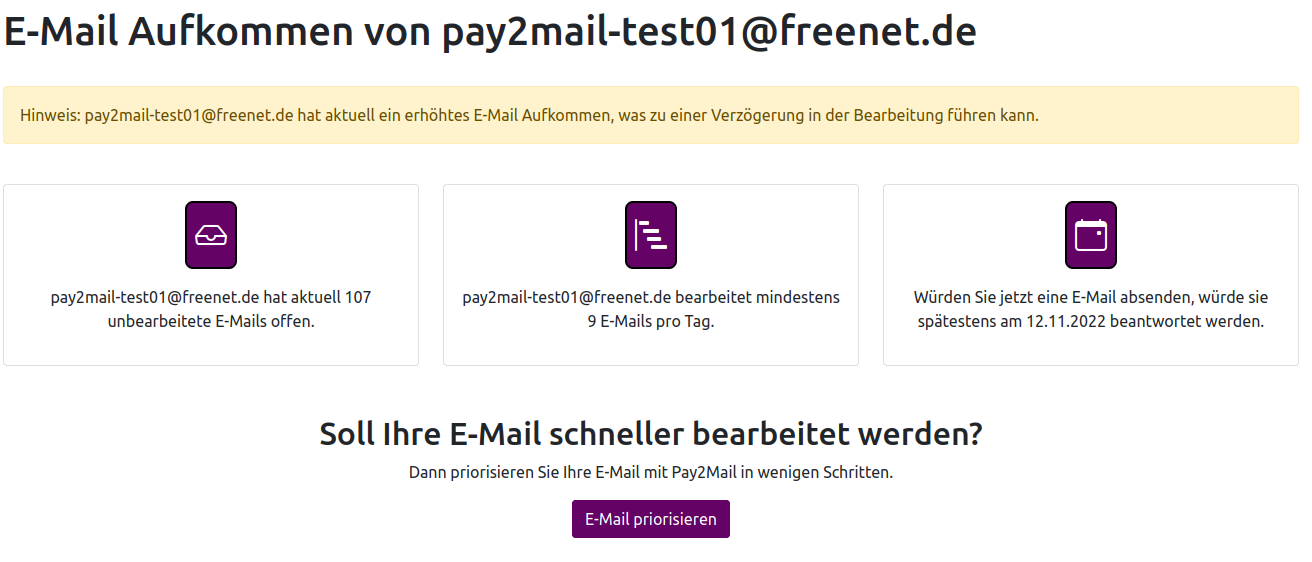
\includegraphics[width=1.2\textwidth]{Figures/send_capacity.png}
	\caption{Screenshot: E-Mail Aufkommen des Empfängers im Prototyp}
	\label{fig:screenshot_send/capacity}
\end{figure}

\begin{figure}[!h]
	\centering
		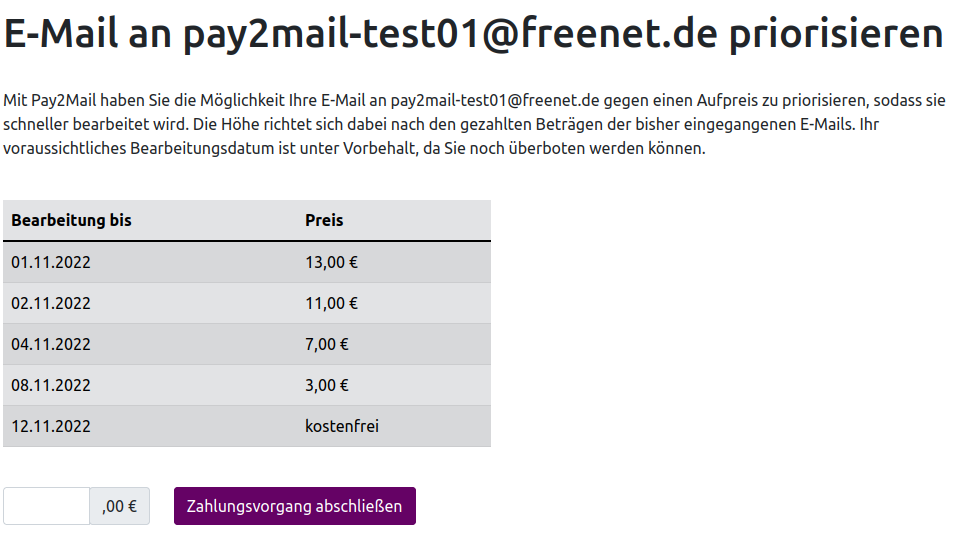
\includegraphics[width=1\textwidth]{Figures/send_priority.png}
	\caption{Screenshot: Priorisierungsmöglichkeiten für Empfänger im Prototyp}
	\label{fig:screenshot_send/priority}
\end{figure}

\newpage
\section{Screenshots des ersten Arbeitspaketes}

\begin{figure}[!h]
	\centering
		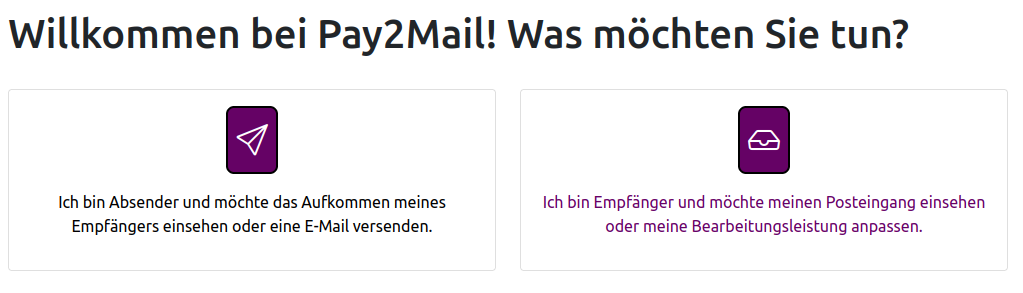
\includegraphics[width=1\textwidth]{Figures/overview.png}
	\caption{Screenshot: Startseite zur Auswahl von Absenderfrontend oder Empfängerfrontend}
	\label{fig:screenshot_overview}
\end{figure}

\newpage
\section{Screenshots des zweiten Arbeitspaketes}

\begin{figure}[!h]
	\centering
		
\includegraphics[width=1\textwidth]{Figures/send_priority_new.png}
	\caption{Screenshot: Formular zur Priorisierung einer E-Mail}
	\label{fig:screenshot_send/priority_new}
\end{figure}

\begin{figure}[!h]
	\centering
		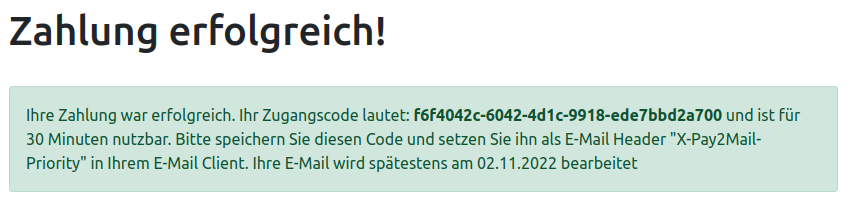
\includegraphics[width=1\textwidth]{Figures/send_priority_show.png}
	\caption{Screenshot: Anzeige eines erstellten Gegenwert-Headers}
	\label{fig:screenshot_send/priority_show}
\end{figure}

\newpage
\section{Screenshots des dritten Arbeitspaketes}

\begin{figure}[!h]
	\centering
		
\includegraphics[width=0.25\textwidth]{Figures/header1.png}
	\caption{Screenshot: Oberer rechter Teil des Headers bei ausgeloggtem Nutzer}
	\label{fig:screenshot_header1}
\end{figure}

\begin{figure}[!h]
	\centering
		
\includegraphics[width=0.5\textwidth]{Figures/header2.png}
	\caption{Screenshot: Oberer rechter Teil des Headers bei eingeloggtem Nutzer}
	\label{fig:screenshot_header2}
\end{figure}

\begin{figure}[!h]
	\centering
		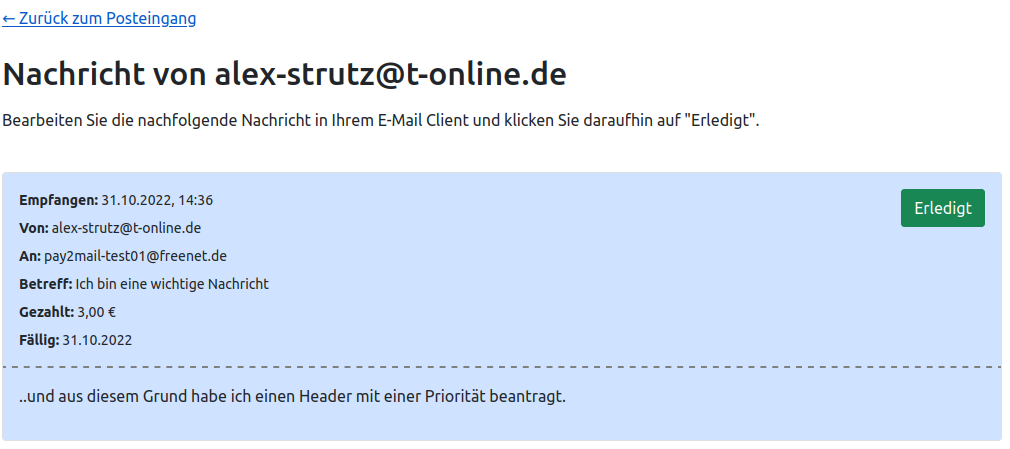
\includegraphics[width=1.1\textwidth]{Figures/message.png}
	\caption{Screenshot: Einzelansicht einer Nachricht für Empfänger}
	\label{fig:screenshot_message}
\end{figure}

\begin{figure}[!h]
	\centering
		
\includegraphics[width=0.6\textwidth]{Figures/tab.png}
	\caption{Screenshot: \texttt{Tab}-Komponente mit Möglichkeit zum Wechseln der Posteingangstabellen}
	\label{fig:screenshot_inbox2}
\end{figure}

\begin{figure}[!h]
	\centering
		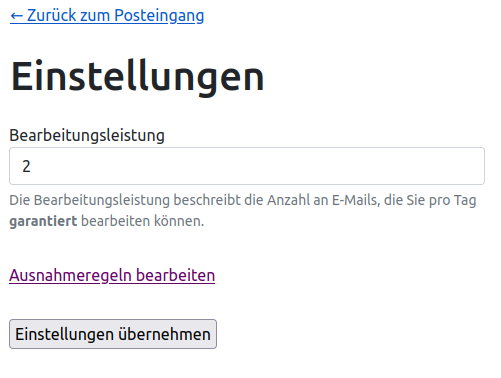
\includegraphics[width=0.75\textwidth]{Figures/recipients.png}
	\caption{Screenshot: Anpassung der Bearbeitungsleistung durch den Empfänger}
	\label{fig:screenshot_recipients}
\end{figure}

\begin{figure}[!h]
	\centering
		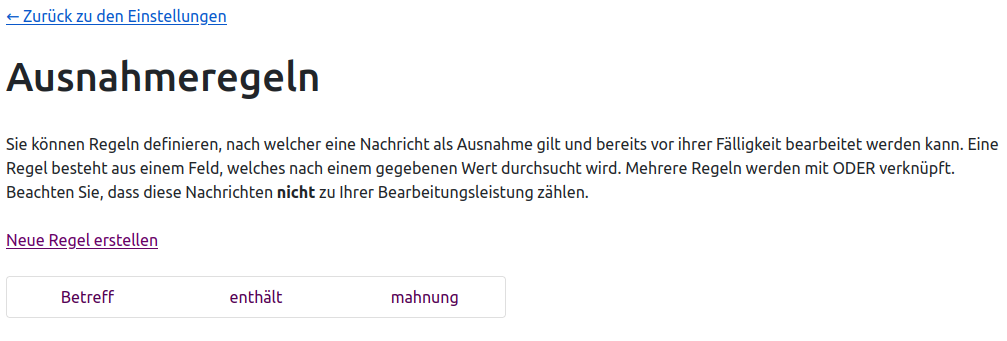
\includegraphics[width=1.1\textwidth]{Figures/rules1.png}
	\caption{Screenshot: Auflistung der definierten Regeln eines Empfängers}
	\label{fig:screenshot_rules1}
\end{figure}

\begin{figure}[!h]
	\centering
		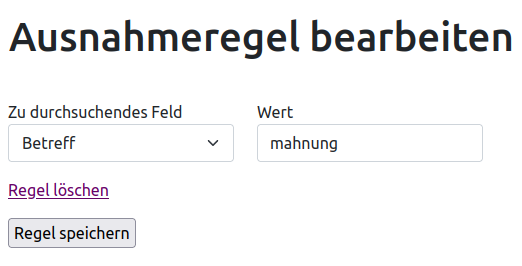
\includegraphics[width=0.75\textwidth]{Figures/rules2.png}
	\caption{Screenshot: Bearbeitung einer Regel durch den Empfänger}
	\label{fig:screenshot_rules2}
\end{figure}

\begin{figure}[!h]
	\centering
		
\includegraphics[width=0.75\textwidth]{Figures/rules3.png}
	\caption{Screenshot: Erstellung einer neuen Regel durch den Empfänger}
	\label{fig:screenshot_rules3}
\end{figure}



%----------------------------------------------------------------------------------------
%	BIBLIOGRAPHY
%----------------------------------------------------------------------------------------

\printbibliography[heading=bibintoc]

%----------------------------------------------------------------------------------------


%----------------------------------------------------------------------------------------
%	DECLARATION PAGE
%----------------------------------------------------------------------------------------

%!TEX root = ../main.tex

\chapter*{Eidesstattliche Erklärung}

\addchaptertocentry{\authorshipname} % Add the declaration to the table of contents

\noindent Ich versichere, die von mir vorgelegte Arbeit selbstständig verfasst zu haben. \\ \\


\noindent Alle Stellen, die wörtlich oder sinngemäß aus veröffentlichten oder nicht veröffentlichten Arbeiten anderer entnommen sind, habe ich als entnommen kenntlich gemacht. Sämtliche Quellen und Hilfsmittel, die ich für die Arbeit benutzt habe, sind angegeben. \\ \\


\noindent Die Arbeit hat mit gleichem Inhalt bzw. in wesentlichen Teilen noch keiner anderen Prüfungsbehörde vorgelegen.

\vspace{1cm}  

\noindent Gummersbach, 9. November 2022  
 
 
\vspace{2.5cm} 
 

\noindent \rule[0.5em]{25em}{0.5pt} \\ % This prints a line for the signature
\noindent \authorname




\end{document}  
